\documentclass[lettersize,journal]{IEEEtran}
\usepackage{amsmath,amsfonts}
\usepackage{algpseudocode}
\algnewcommand\Procedure[2]{\State\textbf{procedure} \textsc{#1}(#2)}
\algnewcommand\EndProcedure{\State\textbf{end procedure}}
\algnewcommand\Function[2]{\State\textbf{function} \textsc{#1}(#2)}
\algnewcommand\EndFunction{\State\textbf{end function}}
\usepackage{algorithm}
\usepackage{array}
\usepackage[caption=false,font=normalsize,labelfont=sf,textfont=sf]{subfig}
\usepackage{textcomp}
\usepackage{stfloats}
\usepackage{url}
\usepackage{verbatim}
\usepackage{graphicx}
\usepackage{cite}
\hyphenation{op-tical net-works semi-conduc-tor IEEE-Xplore}
% updated with editorial comments 8/9/2021

\begin{document}

\title{Design of a Secure Academic Authentication System Based on Blockchain and Decentralized Storage}

\author{Zongyou Yang, Zhouhe Zhang, Zijie Wang, and Yinghan Hou
\thanks{Manuscript received July 13, 2025; revised XX, 2025.}
\thanks{Zongyou Yang is with University College London (UCL), London, UK (e-mail: zongyou.yang@example.com).}
\thanks{Zhouhe Zhang is with the School of Artificial Intelligence, Beijing University of Posts and Telecommunications (BUPT), Beijing, China (e-mail: zhouhe.zhang@example.com).}
\thanks{Zijie Wang is with Kunlun Digital Intelligence (CNPC), Beijing, China (e-mail: zijie.wang@example.com).}
\thanks{Yinghan Hou is with Imperial College London, London, UK (e-mail: yinghan.hou@example.com).}}

% The paper headers
\markboth{Journal of Example, Vol. XX, No. X, July 2025}{Yang: Design of a Secure Academic Authentication System...}

\maketitle

\begin{abstract}
Academic credential fraud is a pervasive global issue that undermines the integrity of educational systems and devalues legitimate qualifications. Traditional verification methods are often centralized, inefficient, and susceptible to forgery. This paper proposes a secure, decentralized academic authentication system leveraging blockchain technology and the InterPlanetary File System (IPFS). The system ensures the immutability and tamper-proof nature of academic records by storing credential hashes on a distributed ledger, while the full credentials are kept in a decentralized storage network. We present a comprehensive system architecture, detail the design of core smart contracts for managing the lifecycle of credentials, and outline a privacy-preserving verification process. The proposed system provides a trustworthy, efficient, and user-centric solution for academic credentialing. Our comprehensive experimental evaluation demonstrates the system's practical viability, achieving sub-5ms latency, O(1) query scalability up to one million records, over 98\% reduction in gas costs, and high resilience to node failures.
\end{abstract}

\begin{IEEEkeywords}
Blockchain, Academic Authentication, Smart Contracts, Decentralized Storage, IPFS, Verifiable Credentials.
\end{IEEEkeywords}

\section{INTRODUCTION}
\IEEEPARstart{A}{CADEMIC} credentials, such as degrees and certificates, are fundamental pillars of trust in modern society. They serve as the primary mechanism for individuals to prove their qualifications and for institutions and employers to verify them. However, the integrity of this trust is increasingly threatened by a global surge in academic fraud. The problem is widespread and multifaceted, ranging from the forgery of transcripts to the creation of entirely fictitious degrees from diploma mills. For instance, a 2010 report estimated that for Chinese student applications to U.S. universities, as many as 90\% of recommendation letters were fabricated and 50\% of high school transcripts were falsified \cite{WES2017Fraud}. Similar systemic issues have been uncovered in various nations, including large-scale admissions fraud in India and the issuance of illegitimate degrees to politicians in Kenya \cite{WES2017Fraud}. This erosion of trust not only devalues legitimate qualifications but also poses significant risks to industries that rely on a verifiably skilled workforce, such as healthcare and engineering.

The conventional methods of credential verification, which are often centralized, paper-based, and reliant on manual checks, are slow, costly, and vulnerable to single points of failure and attack. In response to these challenges, blockchain technology has emerged as a promising solution. Its inherent properties of decentralization, immutability, and cryptographic security offer a robust foundation for building a new generation of tamper-proof and transparent verification systems. By recording credentials or their cryptographic proofs on a distributed ledger, a blockchain-based system can enable instant, secure, and universally accessible verification without relying on a central intermediary.

This paper proposes a comprehensive design for an academic authentication system that leverages blockchain technology, decentralized storage, and modern cryptographic principles to address the critical flaws in traditional verification processes. Our goal is to create a system that is not only secure and resilient against fraud but also respects user privacy and enhances data portability.

Despite the promise of blockchain, many existing academic credentialing systems exhibit significant limitations. Early models often stored extensive data directly on-chain, leading to scalability and privacy issues. Others rely on simple on-chain revocation lists, which fail to protect student privacy by publicly exposing revoked credentials. Furthermore, many systems lack robust, decentralized identity management, tying a user's academic history to a single, fragile key pair and offering no clear path for key rotation or account recovery. This creates a significant research gap for a holistic system that balances immutability, privacy, efficiency, and user-centric control.

To address these challenges, this paper makes the following key contributions:
\begin{itemize}
    \item \textbf{Formal System Architecture:} We design and present a comprehensive, multi-layered architecture that integrates a permissioned blockchain (e.g., Hyperledger Fabric) with the InterPlanetary File System (IPFS). This hybrid approach ensures on-chain integrity for critical data (hashes, DIDs, revocation states) while leveraging off-chain storage for efficiency and privacy.
    \item \textbf{Privacy-Preserving Revocation:} We introduce a novel and efficient credential revocation mechanism based on cryptographic accumulators. This method allows for constant-time revocation checks without revealing any information about the set of revoked credentials, significantly enhancing holder privacy compared to traditional CRLs or simple on-chain lists.
    \item \textbf{Decentralized Identity and Key Management:} We implement a robust identity management system based on the W3C DID standard. Our design, detailed in the \texttt{IdentityManager} contract, supports secure key rotation, history tracking, and a social recovery mechanism, ensuring long-term user control and credential validity even if primary keys are compromised.
    \item \textbf{Comprehensive Performance Evaluation:} We conduct a rigorous, multi-faceted experimental evaluation of the system's performance. Our analysis provides quantitative evidence of the system's: 1) high throughput and low latency for core operations; 2) O(1) query scalability, demonstrating constant-time lookups even with one million records; 3) superior cost-efficiency, with over 98\% gas savings compared to fully on-chain models; 4) highly efficient revocation mechanism; and 5) resilience to node failures in a distributed setting. These results validate the practical viability and robustness of our design.
\end{itemize}

The remainder of this paper is organized as follows. Section II reviews related work in blockchain-based credentialing. Section III details our proposed system architecture and design. Section IV presents the implementation of our core smart contracts. Section V provides a comprehensive performance and security evaluation. Finally, Section VI concludes the paper and discusses future work.

\section{Related Work}
The concept of using blockchain for academic credentialing has gained significant traction, evolving from early proof-of-concepts to more sophisticated systems. This section surveys the landscape of existing work, categorizing it by underlying data models, choice of blockchain platform, and adopted privacy-preserving mechanisms.

\subsection{Data Models and Standards}
The foundation of digital credentialing lies in standardized data models. One of the earliest and most influential projects is \textbf{Blockcerts} \cite{Blockcerts}, introduced by the MIT Media Lab. Blockcerts established an open standard for creating, issuing, viewing, and verifying blockchain-based certificates. It championed the model of storing a hash of the credential on-chain while keeping the full certificate off-chain. However, its data model is relatively rigid and predates the more flexible standards that followed.

More recently, the World Wide Web Consortium (W3C) has standardized \textbf{Verifiable Credentials (VCs)} and \textbf{Decentralized Identifiers (DIDs)} \cite{DIDSurvey2024, SSI2023}. VCs provide a flexible data model for expressing claims, while DIDs offer a framework for decentralized, user-controlled identity \cite{SoKVC2023}. Many modern systems have embraced this stack for its interoperability and holder-centric approach \cite{NovelAuthScheme2024, BlockchainDVC2023}. Our work builds upon the W3C standards to leverage their flexibility and broad industry support.

\subsection{Blockchain Platforms for Academic Credentials}
Researchers have explored both public and permissioned blockchains for academic credentialing. Public blockchains like \textbf{Ethereum} offer high decentralization and censorship resistance, and several systems have been proposed on this platform \cite{EthDIDVC}. However, they often suffer from high transaction fees (gas costs), lower throughput, and privacy concerns due to the public nature of the ledger.

In contrast, permissioned blockchains like \textbf{Hyperledger Fabric} provide a more controlled environment suitable for enterprise and consortium applications \cite{FabricEdu}. They offer higher performance, no transaction fees in the traditional sense, and fine-grained access control, making them a strong candidate for inter-institutional academic networks \cite{CredenceLedger2018}. Our system adopts a permissioned blockchain model to ensure scalability, cost-effectiveness, and control over network participation, which is crucial for educational institutions.

\subsection{Privacy-Preserving Mechanisms and Revocation}
A critical challenge in credentialing systems is balancing transparency with privacy, especially during revocation. The simplest approach, an on-chain list of revoked credential IDs, is transparent but severely compromises privacy. The W3C's \texttt{RevocationList2020} standard \cite{RevocationList2020} improves upon this but still requires proofs that can grow with the list size.

To provide stronger privacy, researchers have explored advanced cryptographic techniques. Zero-Knowledge Proofs (ZKPs) can be used to prove statements about credentials without revealing the underlying data \cite{ZKP2023}. Another powerful primitive is the \textbf{cryptographic accumulator}. As detailed in recent studies \cite{AccumulatorCrypto2024}, accumulators can represent a large set of values with a single, constant-size string. This allows for highly efficient and private revocation checks, as a user can generate a non-membership proof to demonstrate their credential is not in the revocation set without learning about any other revoked credential. Our work's core innovation lies in the practical application and implementation of a cryptographic accumulator for scalable and private revocation, a significant step beyond simple on-chain lists.

\subsection{Decentralized Identity and Key Management}
Securely managing the lifecycle of digital identities is paramount. A lost key could mean the loss of one's entire academic history. Recent work on DID has focused on robust key management models, including key rotation and recovery mechanisms \cite{KeyManagement2024}. Systems like CanDID have proposed architectures that incorporate threshold-based guardians for account recovery \cite{CanDID2021}. Our \texttt{IdentityManager} contract is heavily inspired by this line of research, implementing both key rotation and a social recovery scheme to provide a resilient and user-centric identity management solution.



\section{System Design and Architecture}

Our proposed system is designed to be secure, private, and user-centric. This section details the formal system model, the overall architecture, and the core operational workflows.

\subsection{System Model and Goals}
We define a system model consisting of three primary actors:
\begin{itemize}
    \item \textbf{Issuing Institutions (Issuers):} Trusted entities, such as universities or colleges, that are authorized to create and issue academic credentials. They are responsible for verifying a student's achievements before issuing a corresponding VC.
    \item \textbf{Credential Holders (Holders):} Individuals, typically students or alumni, who receive credentials from issuers. They have full control over their credentials and decide when and with whom to share them.
    \item \textbf{Verifiers:} Third parties, such as employers or other academic institutions, that need to verify the authenticity and validity of a holder's credentials.
\end{itemize}

Our design is guided by the following core goals:
\begin{itemize}
    \item \textbf{Integrity and Authenticity:} It must be computationally infeasible to forge or tamper with academic credentials. Verifiers must be able to reliably trace any credential back to its legitimate issuer.
    \item \textbf{Privacy:} The system must not expose the personal information of holders. Specifically, the act of verifying or revoking a credential should not reveal sensitive data to unauthorized parties.
    \item \textbf{User Control and Portability:} Holders must have ultimate control over their own data (self-sovereign identity). Credentials should be portable and not locked into any single platform or vendor.
    \item \textbf{Availability and Efficiency:} The verification process must be highly available and efficient, without relying on the original issuer to be online.
\end{itemize}

\subsection{System Architecture}
To achieve these goals, we propose a multi-layered architecture that separates on-chain and off-chain concerns, as depicted in Fig. \ref{fig:architecture}. The architecture consists of a permissioned blockchain, a decentralized storage network, and client-side applications.

% \begin{figure}[!t]
% \centering
% \includegraphics[width=3.5in]{figures/architecture_diagram.png}
% \caption{The proposed system architecture, illustrating the interaction between the Holder, Issuer, and Verifier with the permissioned blockchain and the IPFS decentralized storage network.}
% \label{fig:architecture}
% \end{figure}

\begin{itemize}
    \item \textbf{Blockchain Layer:} We utilize a permissioned blockchain (e.g., Hyperledger Fabric) to serve as the root of trust. The ledger stores immutable records critical for verification, including issuer DIDs, credential metadata (e.g., cryptographic hashes, issuer signatures), and the state of the revocation accumulator. It does not store any personally identifiable information (PII).
    \item \textbf{Storage Layer:} We use the InterPlanetary File System (IPFS) for off-chain storage of the actual Verifiable Credentials \cite{IPFS2023}. When an issuer creates a credential, the JSON-LD document is stored on IPFS, which returns a unique Content Identifier (CID). This CID, which is a hash of the content, is what gets recorded on the blockchain. This "on-chain hash, off-chain data" pattern ensures data integrity while enhancing privacy and scalability.
    \item \textbf{Application Layer:} This layer includes the client-side applications (e.g., digital wallets) used by holders, issuers, and verifiers to interact with the system. For instance, a holder's wallet stores their private keys and VCs, and provides the interface for presenting credentials to verifiers.
\end{itemize}

\subsection{Core Workflows}
The primary operations within the system are credential issuance, verification, and revocation. The interactions are illustrated in the sequence diagram in Fig.~\ref{fig:sequence}.

% \begin{figure}[!t]
% \centering
% \includegraphics[width=3.5in]{figures/sequence_diagram.png}
% \caption{Sequence diagram illustrating the core workflows: 1) Credential Issuance, 2) Credential Presentation and Verification, and 3) Credential Revocation.}
% \label{fig:sequence}
% \end{figure}

\begin{enumerate}
    \item \textbf{Credential Issuance:} An issuer generates a VC for a holder, signs it with their private key, and stores the VC on IPFS. The issuer then invokes the \texttt{CredentialRegistry} smart contract, recording the IPFS CID and other metadata on the blockchain.
    \item \textbf{Credential Verification:} The holder presents the VC (retrieved from IPFS) to a verifier. The verifier first checks the cryptographic signature on the VC itself. Then, it queries the blockchain using the credential's hash to confirm its registration. Finally, it interacts with the \texttt{RevocationRegistry} contract to ensure the credential has not been revoked.
    \item \textbf{Credential Revocation:} If an issuer needs to revoke a credential, it sends a transaction to the \texttt{RevocationRegistry} contract. The contract updates the cryptographic accumulator to reflect this change, ensuring that any future verification attempts for this credential will fail.
\end{enumerate}

\section{Smart Contract Implementation}

The core functionality of our system is implemented through a set of smart contracts that manage the lifecycle of credentials.

\subsection{Core Smart Contracts}
We have developed three primary smart contracts that handle the core functionality of the system:

\subsubsection{CredentialRegistry Contract} This contract manages the registration, verification, and lifecycle of credentials. Below is a simplified version of the key functions:

\begin{algorithm}
\caption{Pseudo-code of CredentialRegistry Contract}
\label{alg:credential_registry}
\begin{algorithmic}[1]
\STATE \textbf{function} registerCredential(issuerDID, holderDID, credentialCID, metadata)
\STATE \quad \textbf{require} msg.sender == issuerMapping[issuerDID]
\STATE \quad credID = generateUniqueID()
\STATE \quad credentials[credID] = Credential(\{
\STATE \quad \quad issuerDID: issuerDID, 
\STATE \quad \quad holderDID: holderDID, 
\STATE \quad \quad cid: credentialCID, 
\STATE \quad \quad issuanceDate: now(), 
\STATE \quad \quad status: ”ACTIVE”, 
\STATE \quad \quad metadata: metadata\})
\STATE \quad emit CredentialRegistered(credID, issuerDID, holderDID)
\STATE \quad \textbf{return} credID
\STATE \textbf{end function}
\STATE
\STATE \textbf{function} verifyCredentialStatus(credentialID)
\STATE \quad credential = credentials[credentialID]
\STATE \quad \textbf{require} credential.exists()
\STATE \quad revocationStatus = RevocationRegistry.checkStatus(credentialID)
\STATE \quad \textbf{return} \{status: credential.status, revoked: revocationStatus\}
\STATE \textbf{end function}
\end{algorithmic}
\end{algorithm}

\subsubsection{RevocationRegistry Contract} This contract implements our novel revocation mechanism using cryptographic accumulators, which enables efficient revocation checks without revealing which specific credentials have been revoked, thereby protecting holder privacy.

\begin{algorithm}
\caption{Pseudo-code of RevocationRegistry Contract}
\label{alg:revocation_registry}
\begin{algorithmic}[1]
\STATE \textbf{function} revokeCredential(issuerDID, credentialID, reason)
\STATE \quad \textbf{require} msg.sender == issuerMapping[issuerDID]
\STATE \quad credential = CredentialRegistry.getCredential(credentialID)
\STATE \quad \textbf{require} credential.issuerDID == issuerDID
\STATE \quad \textbf{if} !revocationAccumulators[issuerDID].contains(credentialID) \textbf{then}
\STATE \quad \quad accumulatorValue = revocationAccumulators[issuerDID].value
\STATE \quad \quad newAccValue = accumulatorAdd(accumulatorValue, credentialID)
\STATE \quad \quad revocationAccumulators[issuerDID].value = newAccValue
\STATE \quad \quad revocationAccumulators[issuerDID].lastUpdated = now()
\STATE \quad \quad emit CredentialRevoked(credentialID, issuerDID, reason)
\STATE \quad \textbf{end if}
\STATE \textbf{end function}
\STATE
\STATE \textbf{function} checkStatus(credentialID)
\STATE \quad credential = CredentialRegistry.getCredential(credentialID)
\STATE \quad issuerDID = credential.issuerDID
\STATE \quad accValue = revocationAccumulators[issuerDID].value
\STATE \quad \textbf{return} accumulatorContains(accValue, credentialID)
\STATE \textbf{end function}

\Procedure{verifyNonRevocationProof}{credentialID, nonRevocationProof}
    \State $credential \gets CredentialRegistry.getCredential(credentialID)$
    \State $issuerDID \gets credential.issuerDID$
    \State $accData \gets revocationAccumulators[issuerDID]$
    
    \Comment{Verify the proof was generated for the current accumulator value}
    \Require $nonRevocationProof.accumulator = accData.value$ \Comment{Prevent outdated proofs}
    
    \Comment{Verify the zero-knowledge proof}
    \State $valid \gets verifyZKNonMembershipProof(accData.value, nonRevocationProof.zkProof)$
    
    \RETURN $valid$
\EndProcedure
\end{algorithmic}
\end{algorithm} 

\begin{algorithm}
\caption{Undo Revocation Procedure}
\begin{algorithmic}[1]
\Procedure{undoRevocation}{issuerDID, credentialID, adminSignature}
    \Require $isAdmin(msg.sender)$ \Comment{Only admin can undo revocations}
    \Require $verifyAdminSignature(adminSignature)$ \Comment{Valid signature required}
    
    \State $record \gets revocationRecords[issuerDID][credentialID]$
    \Require $record.timestamp > 0$ \Comment{Credential must be revoked}
    
    \Comment{This is an expensive operation requiring re-initialization of the accumulator}
    \Comment{and re-addition of all other revoked credentials except this one}
    \State $recomputeAccumulator(issuerDID, credentialID)$
    
    \Comment{Remove from revocation records}
    \State $delete\ revocationRecords[issuerDID][credentialID]$
    
    \Comment{Remove from issuer's revocation list}
    \State $removeFromArray(issuerRevocations[issuerDID], credentialID)$
    
    \Comment{Update revocation count}
    \State $revocationAccumulators[issuerDID].revocationCount \gets revocationAccumulators[issuerDID].revocationCount - 1$
    
    \State \textsc{emit} $RevocationUndone(issuerDID, credentialID)$
    \RETURN true
\EndProcedure
\end{algorithmic}
\end{algorithm}

\subsubsection{Mathematical Details of the Accumulator Implementation}

Our revocation mechanism uses an RSA-based cryptographic accumulator with the following properties:

\begin{itemize}
    \item \textbf{One-Way Accumulator:} Based on the strong RSA assumption, making it computationally infeasible to find the accumulated values given only the accumulator.
    
    \item \textbf{Quasi-Commutative:} The order of adding elements to the accumulator does not affect the final value, ensuring consistency regardless of the order of revocations.
    
    \item \textbf{Prime Representative Mapping:} Credential IDs are mapped to prime numbers using a deterministic hash-to-prime algorithm to prevent collisions and ensure security.
\end{itemize}

The core mathematical operations are defined as follows:

\begin{itemize}
    \item \textbf{Accumulator Initialization:} $Acc_0 = g^{1} \mod N$ where $g$ is a generator and $N$ is an RSA modulus.
    
    \item \textbf{Adding a value:} $Acc_i = Acc_{i-1}^{e_i} \mod N$ where $e_i$ is the prime representative of credential $i$.
    
    \item \textbf{Membership Verification:} Testing if $Acc_i = Acc_{i-1}^{e_i} \mod N$ confirms if $e_i$ is in the accumulator.
    
    \item \textbf{Non-Membership Witness:} For a value $x$ not in accumulator $Acc_X$, a witness $(a, b)$ satisfies $g^a \cdot x^b = Acc_X \mod N$.
\end{itemize}

This approach provides several advantages for our academic credential system:

\begin{itemize}
    \item \textbf{Privacy Preservation:} Verifiers can check if a specific credential is revoked without learning about other revoked credentials.
    
    \item \textbf{Compact Representation:} A single accumulator value represents the entire set of revoked credentials, regardless of the set size.
    
    \item \textbf{Efficient Verification:} Verification requires only a small constant number of modular exponentiations.
\subsubsection{3. IdentityManager Contract}
This contract handles DID registration, key management, and recovery mechanisms. It enables secure updates of cryptographic keys without invalidating existing credentials.

\begin{algorithm}[H]
\caption{Enhanced Pseudo-code of IdentityManager Contract}
\begin{algorithmic}[1]
\Statex \textbf{// Data structures}
\Statex \textit{struct Identity \{}
\Statex \hspace{\algorithmicindent} \textit{string did; // Decentralized Identifier}
\Statex \hspace{\algorithmicindent} \textit{string[] publicKeys; // Array of public keys (current and historical)}
\Statex \hspace{\algorithmicindent} \textit{mapping(uint256 => KeyData) keyHistory; // Key history with timestamps}
\Statex \hspace{\algorithmicindent} \textit{address[] controllers; // Addresses that can control this identity}
\Statex \hspace{\algorithmicindent} \textit{address[] recoveryAgents; // Agents authorized for recovery}
\Statex \hspace{\algorithmicindent} \textit{uint256 thresholdSignatureCount; // Required signatures for recovery}
\Statex \hspace{\algorithmicindent} \textit{string metadataCID; // IPFS CID for additional identity metadata}
\Statex \hspace{\algorithmicindent} \textit{bool active; // Identity status flag}
\Statex \textit{\}}
\Statex 
\Statex \textit{struct KeyData \{}
\Statex \hspace{\algorithmicindent} \textit{string keyId; // Key identifier}
\Statex \hspace{\algorithmicindent} \textit{string publicKey; // Public key material}
\Statex \hspace{\algorithmicindent} \textit{string keyType; // Type of key (e.g., ECDSA, EdDSA)}
\Statex \hspace{\algorithmicindent} \textit{uint256 addedTimestamp; // When this key was added}
\Statex \hspace{\algorithmicindent} \textit{uint256 revokedTimestamp; // When this key was revoked (0 if active)}
\Statex \hspace{\algorithmicindent} \textit{string purpose; // Key purpose (authentication, assertion, etc.)}
\Statex \textit{\}}
\Statex 
\Statex \textbf{// State variables}
\Statex \textit{mapping(string => Identity) identities; // DID -> Identity}
\Statex \textit{mapping(address => string[]) controlledIdentities; // Controller address -> array of DIDs}
\Statex 

\Function{createIdentity}{publicKey, keyType, controllers, recoveryAgents, threshold, metadataCID}
    \State \textbf{require} controllers.length > 0, "At least one controller required"
    \State \textbf{require} recoveryAgents.length >= threshold, "Insufficient recovery agents"
    
    \State // Generate DID based on method-specific algorithm
    \State string did = generateDID("fabric", publicKey, now());
    \State \textbf{require} !identities[did].exists(), "DID already exists"
    
    \State // Create key data for initial key
    \State string keyId = concat(did, "#key-1")
    \State KeyData memory initialKey = KeyData(\{
        \hspace{\algorithmicindent}keyId: keyId,
        \hspace{\algorithmicindent}publicKey: publicKey,
        \hspace{\algorithmicindent}keyType: keyType,
        \hspace{\algorithmicindent}addedTimestamp: now(),
        \hspace{\algorithmicindent}revokedTimestamp: 0,
        \hspace{\algorithmicindent}purpose: "authentication"
    \})
    
    \State // Create identity record
    \State Identity memory identity = Identity(\{
        \hspace{\algorithmicindent}did: did,
        \hspace{\algorithmicindent}controllers: controllers,
        \hspace{\algorithmicindent}recoveryAgents: recoveryAgents,
        \hspace{\algorithmicindent}thresholdSignatureCount: threshold,
        \hspace{\algorithmicindent}metadataCID: metadataCID,
        \hspace{\algorithmicindent}active: true
    \})
    
    \State // Add initial key
    \State identity.publicKeys.push(keyId)
    \State identity.keyHistory[0] = initialKey
    
    \State // Store identity and controller relationships
    \State identities[did] = identity
    \State \textbf{for} each controller in controllers \textbf{do}
        \State \hspace{\algorithmicindent} controlledIdentities[controller].push(did)
    \State \textbf{end for}
    
    \State \textbf{emit} IdentityCreated(did, controllers, now())
    \State \textbf{return} did
\EndFunction
\Statex 

\Function{addKey}{did, newPublicKey, keyType, purpose, signature}
    \State Identity storage identity = identities[did]
    \State \textbf{require} identity.exists(), "Identity does not exist"
    \State \textbf{require} isAuthorizedController(msg.sender, did), "Not authorized"
    
    \State // Verify controller signature
    \State \textbf{require} verifyControllerSignature(did, signature), "Invalid signature"
    
    \State // Create new key data
    \State string keyId = concat(did, "#key-", (identity.publicKeys.length + 1))
    \State KeyData memory newKey = KeyData(\{
        \hspace{\algorithmicindent}keyId: keyId,
        \hspace{\algorithmicindent}publicKey: newPublicKey,
        \hspace{\algorithmicindent}keyType: keyType,
        \hspace{\algorithmicindent}addedTimestamp: now(),
        \hspace{\algorithmicindent}revokedTimestamp: 0,
        \hspace{\algorithmicindent}purpose: purpose
    \})
    
    \State // Add key to identity
    \State identity.publicKeys.push(keyId)
    \State identity.keyHistory[identity.publicKeys.length - 1] = newKey
    
    \State \textbf{emit} KeyAdded(did, keyId, now())
    \State \textbf{return} keyId
\EndFunction
\Statex 

\Function{revokeKey}{did, keyId, signature}
    \State Identity storage identity = identities[did]
    \State \textbf{require} identity.exists(), "Identity does not exist"
    \State \textbf{require} isAuthorizedController(msg.sender, did), "Not authorized"
    \State \textbf{require} verifyControllerSignature(did, signature), "Invalid signature"
    
    \State // Find key in history
    \State bool found = false
    \State uint256 keyIndex = 0
    \State \textbf{for} i = 0; i < identity.publicKeys.length; i++ \textbf{do}
        \State \hspace{\algorithmicindent} \textbf{if} identity.keyHistory[i].keyId == keyId \textbf{then}
            \State \hspace{\algorithmicindent}\hspace{\algorithmicindent} found = true
            \State \hspace{\algorithmicindent}\hspace{\algorithmicindent} keyIndex = i
            \State \hspace{\algorithmicindent}\hspace{\algorithmicindent} \textbf{break}
        \State \hspace{\algorithmicindent} \textbf{end if}
    \State \textbf{end for}
    
    \State \textbf{require} found, "Key not found"
    \State \textbf{require} identity.keyHistory[keyIndex].revokedTimestamp == 0, "Key already revoked"
    
    \State // Ensure at least one active key remains
    \State uint256 activeKeyCount = 0
    \State \textbf{for} i = 0; i < identity.publicKeys.length; i++ \textbf{do}
        \State \hspace{\algorithmicindent} \textbf{if} identity.keyHistory[i].revokedTimestamp == 0 \textbf{then}
            \State \hspace{\algorithmicindent}\hspace{\algorithmicindent} activeKeyCount++
        \State \hspace{\algorithmicindent} \textbf{end if}
    \State \textbf{end for}
    \State \textbf{require} activeKeyCount > 1, "Cannot revoke last active key"
    
    \State // Revoke the key
    \State identity.keyHistory[keyIndex].revokedTimestamp = now()
    
    \State \textbf{emit} KeyRevoked(did, keyId, now())
\EndFunction
\Statex 

\Function{recoverIdentity}{did, newController, signatures}
    \State Identity storage identity = identities[did]
    \State \textbf{require} identity.exists(), "Identity does not exist"
    \State \textbf{require} signatures.length >= identity.thresholdSignatureCount, "Insufficient signatures"
    
    \State // Verify recovery agent signatures
    \State uint256 validSignatures = 0
    \State \textbf{for} i = 0; i < signatures.length; i++ \textbf{do}
        \State \hspace{\algorithmicindent} address recoveryAgent = recoverSigner(signatures[i], did)
        \State \hspace{\algorithmicindent} \textbf{if} isRecoveryAgent(did, recoveryAgent) \textbf{then}
            \State \hspace{\algorithmicindent}\hspace{\algorithmicindent} validSignatures++
        \State \hspace{\algorithmicindent} \textbf{end if}
    \State \textbf{end for}
    
    \State \textbf{require} validSignatures >= identity.thresholdSignatureCount, "Invalid signatures"
    
    \State // Update controllers
    \State \textbf{for} each controller in identity.controllers \textbf{do}
        \State \hspace{\algorithmicindent} removeFromArray(controlledIdentities[controller], did)
    \State \textbf{end for}
    
    \State identity.controllers = [newController]
    \State controlledIdentities[newController].push(did)
    
    \State \textbf{emit} IdentityRecovered(did, newController, now())
\EndFunction
\Statex 

\Function{getActivePublicKey}{did}
    \State Identity storage identity = identities[did]
    \State \textbf{require} identity.exists(), "Identity does not exist"
    
    \State // Find most recently added non-revoked key
    \State string activeKeyId = ""
    \State uint256 latestTimestamp = 0
    
    \State \textbf{for} i = 0; i < identity.publicKeys.length; i++ \textbf{do}
        \State \hspace{\algorithmicindent} KeyData storage key = identity.keyHistory[i]
        \State \hspace{\algorithmicindent} \textbf{if} key.revokedTimestamp == 0 && key.addedTimestamp > latestTimestamp \textbf{then}
            \State \hspace{\algorithmicindent}\hspace{\algorithmicindent} activeKeyId = key.keyId
            \State \hspace{\algorithmicindent}\hspace{\algorithmicindent} latestTimestamp = key.addedTimestamp
        \State \hspace{\algorithmicindent} \textbf{end if}
    \State \textbf{end for}
    
    \State \textbf{require} activeKeyId != "", "No active key found"
    \State \textbf{return} identity.keyHistory[activeKeyId]
\EndFunction
\end{algorithmic}
\end{algorithm}

The IdentityManager contract implements several critical features for maintaining the long-term validity of academic credentials:

\begin{itemize}
    \item \textbf{Key Rotation:} Supporting secure updates to cryptographic keys without invalidating existing credentials.
    
    \item \textbf{Social Recovery:} Implementing an $m$-of-$n$ threshold signature scheme for identity recovery in case of key loss.
    
    \item \textbf{Historical Verification:} Maintaining a complete history of all keys associated with a DID, enabling verification of credentials signed with previous keys.
    
    \item \textbf{Granular Access Control:} Supporting multiple controllers with different permissions for identity management.
\end{itemize}

\subsection{Novel Revocation Mechanism}
A key innovation in our system is the privacy-preserving revocation mechanism based on cryptographic accumulators \cite{AccumulatorCrypto2024}. Unlike traditional revocation lists that grow linearly with the number of revoked credentials and potentially leak information about revoked credentials, our approach offers constant-time verification with enhanced privacy guarantees.

\subsubsection{Limitations of Existing Approaches}
Existing credential revocation mechanisms suffer from several limitations:

\begin{itemize}
    \item \textbf{Certificate Revocation Lists (CRLs):} Require downloading and processing the entire list, which grows linearly with the number of revocations.
    
    \item \textbf{Online Certificate Status Protocol (OCSP):} Requires online connectivity to a central verification server, creating privacy and availability concerns.
    
    \item \textbf{Simple Revocation Lists on Blockchain:} While tamper-proof, they expose all revoked credential IDs, violating holder privacy.
    
    \item \textbf{Verifiable Credentials Revocation List 2020} \cite{RevocationList2020}: Improves on traditional approaches but still requires larger proofs as the list grows.
\end{itemize}

\subsubsection{Our Cryptographic Accumulator Approach}
Our system uses RSA-based cryptographic accumulators with the following advantages:

\begin{align}
    Acc_{X} = g^{\prod_{x_i \in X} e_i} \bmod N
\end{align}

where $X$ is the set of revoked credential identifiers, $g$ is a generator, $N$ is an RSA modulus, and $e_i$ is the prime representative of credential identifier $x_i$.

For credential verification, we use non-membership witnesses. For a credential with identifier $y$ not in the set $X$, there exist integers $a$ and $b$ such that:

\begin{align}
    g^a \cdot y^b = Acc_{X} \bmod N
\end{align}

This witness $(a,b)$ proves that $y$ is not in the accumulator (i.e., not revoked) without revealing any information about which credentials are actually in the revocation accumulator.

\subsubsection{Zero-Knowledge Non-Revocation Proofs}
To further enhance privacy, we implement zero-knowledge proofs \cite{ZKP2023} that allow a holder to prove their credential has not been revoked without revealing the credential identifier. This is particularly important for sensitive academic credentials like medical degrees or special accommodations.

The zero-knowledge proof $\pi$ satisfies:

\begin{align}
    Verify(\pi, (Acc_X, pk_{issuer}), \emptyset) = 1
\end{align}

where the holder proves knowledge of a valid credential and corresponding non-membership witness without revealing any other information.

\subsubsection{Dual Accumulator Architecture: RSA and Bilinear-Map Accumulators}

Our system implements a novel dual accumulator architecture for credential revocation to balance security, privacy, and performance considerations. While the primary accumulator is based on RSA as described above, we also implement a secondary bilinear-map accumulator for specific use cases requiring additional performance optimizations or different security guarantees.

The bilinear-map accumulator is constructed as follows:

\begin{align}
Acc_{BM} = e(g, g)^{\prod_{x_i \in X} (s + x_i)}
\end{align}

where:
\begin{itemize}
    \item $e: \mathbb{G}_1 \times \mathbb{G}_1 \rightarrow \mathbb{G}_T$ is a bilinear map over elliptic curve groups
    \item $g$ is a generator of the group $\mathbb{G}_1$
    \item $s$ is a trapdoor secret known only to the accumulator manager
    \item $X$ is the set of revoked credential identifiers
\end{itemize}

\paragraph{Witness Computation} For a credential $y \notin X$, the non-membership witness $w_y$ is computed as:

\begin{align}
w_y = g^{\prod_{x_i \in X} \frac{s + x_i}{s + y}}
\end{align}

\paragraph{Verification} Verification is efficient and requires checking:

\begin{align}
e(w_y, g^{s+y}) = Acc_{BM}
\end{align}

\paragraph{Advantages of Dual Accumulator Architecture}
Our dual accumulator approach offers several advantages:
\begin{itemize}
    \item \textbf{Security Diversity:} Different cryptographic hardness assumptions (RSA vs. discrete logarithm) provide security against different types of attacks.
    \item \textbf{Performance Options:} Bilinear-map accumulators typically offer faster verification, while RSA accumulators provide more efficient witness updates.
    \item \textbf{Fallback Mechanism:} In case vulnerabilities are discovered in one accumulator type, the system can fall back to the other.
    \item \textbf{Application-Specific Selection:} Different use cases can leverage the most appropriate accumulator type based on their requirements.
\end{itemize}

\begin{equation}
    acc = g^{\prod_{i=1}^{n} (s + x_i)}
\end{equation}

where $g$ is the generator, $s$ is a trapdoor value, and $x_i$ are the revoked credential identifiers. This approach offers:

\begin{itemize}
    \item \textbf{Constant-Size Representation:} The accumulator has a fixed size regardless of how many credentials are revoked.
    \item \textbf{Efficient Verification:} Using pairings, verification is constant-time.
    \item \textbf{Privacy-Preserving:} Checking if a specific credential is revoked does not reveal information about other revoked credentials.
\end{itemize}

\subsection{Smart Contract Interactions and System Workflows}

Our system's smart contracts interact in sophisticated patterns to support the complete credential lifecycle. Figure \ref{fig:contract_interactions} illustrates the key interactions between our core contracts.

% \begin{figure}[h]
% \centering
% \includegraphics[width=0.8\textwidth]{figures/contract_interactions.png}
% \caption{Smart Contract Interactions in the Academic Credential System}
% \label{fig:contract_interactions}
% \end{figure}

\subsubsection{Credential Issuance Workflow}
The credential issuance workflow involves multiple steps across different contracts:

\begin{algorithm}[H]
\caption{Credential Issuance Workflow}
\begin{algorithmic}[1]
\State \Comment{Step 1: Verify issuer's identity}
\State issuerDID $\gets$ IdentityManager.getActiveDID(issuerAddress)
\State \Require IdentityManager.isActive(issuerDID), "Issuer identity inactive"
\State publicKey $\gets$ IdentityManager.getActivePublicKey(issuerDID)

\State \Comment{Step 2: Generate credential content and store off-chain}
\State credContent $\gets$ generateCredentialContent(holderDID, attributes, metadata)
\State contentCID $\gets$ storeCredentialOffChain(credContent) \Comment{Store in IPFS}

\State \Comment{Step 3: Generate cryptographic proof}
\State signatureValue $\gets$ issuerSignature(hashCredentialContent(credContent), issuerPrivateKey)
\State proofValue $\gets$ generateCredentialProof(contentCID, signatureValue, credentialMetadata)

\State \Comment{Step 4: Register credential on-chain}
\State credentialID $\gets$ CredentialRegistry.registerCredential(
\hspace{\algorithmicindent}issuerDID, 
\hspace{\algorithmicindent}holderDID, 
\hspace{\algorithmicindent}contentCID, 
\hspace{\algorithmicindent}schemaID, 
\hspace{\algorithmicindent}expirationDate,
\hspace{\algorithmicindent}proofValue,
\hspace{\algorithmicindent}metadata)

\State \Comment{Step 5: Initialize non-revocation status}
\State nonRevocationWitness $\gets$ RevocationRegistry.generateInitialWitness(credentialID, issuerDID)
\end{algorithmic}
\end{algorithm}

\subsubsection{Credential Verification Workflow}
Verification leverages both on-chain and off-chain components for efficiency and privacy:

\begin{algorithm}[H]
\caption{Credential Verification Workflow}
\begin{algorithmic}[1]
\State \Comment{Step 1: Retrieve credential metadata from blockchain}
\State credentialMetadata $\gets$ CredentialRegistry.getCredential(credentialID)
\State issuerDID $\gets$ credentialMetadata.issuerDID
\State contentCID $\gets$ credentialMetadata.contentCID

\State \Comment{Step 2: Check credential status}
\State isRevoked $\gets$ RevocationRegistry.checkRevocationStatus(credentialID)
\If{isRevoked \textbf{or} now() > credentialMetadata.expirationDate}
\RETURN "Invalid credential"
\EndIf

\State \Comment{Step 3: Retrieve credential content from IPFS}
\State credentialContent $\gets$ retrieveFromIPFS(contentCID)

\State \Comment{Step 4: Get issuer's public key}
\State issuerKeyId $\gets$ IdentityManager.getKeyIdAtTime(issuerDID, credentialMetadata.issuanceDate)
\State issuerPublicKey $\gets$ IdentityManager.getPublicKeyByKeyId(issuerDID, issuerKeyId)

\State \Comment{Step 5: Verify the cryptographic proof}
\State contentHash $\gets$ hashCredentialContent(credentialContent)
\State isValidSignature $\gets$ verifySignature(contentHash, credentialMetadata.proofValue, issuerPublicKey)

\State \Comment{Step 6: Validate selective disclosure proofs (if applicable)}
\If{credentialContent.hasSelectiveDisclosure()}
\State isValidProof $\gets$ verifyZKProof(credentialContent.zkProof, issuerPublicKey)
\State \Require isValidProof, "Invalid selective disclosure proof"
\EndIf

\RETURN isValidSignature ? "Valid credential" : "Invalid credential"
\end{algorithmic}
\end{algorithm}

The revocation process maintains privacy while ensuring efficient verification:

\begin{algorithm}[H]
\caption{Credential Revocation Workflow}
\begin{algorithmic}[1]
\Procedure{revokeCredential}{credentialID, revocationReason}
    \Require msg.sender = issuerMapping[credentialID.issuerDID]
    \State RevocationRegistry.revokeCredential(credentialID, revocationReason)
    \State CredentialRegistry.updateCredentialStatus(credentialID, "REVOKED", revocationReason)
    \State \textsc{emit} CredentialRevoked(credentialID, revocationReason)
\EndProcedure
\end{algorithmic}
\end{algorithm}

\subsubsection{Privacy-Preserving Selective Disclosure}
Our system supports selective disclosure of credential attributes using zero-knowledge proofs \cite{ZKP2023}:

\begin{algorithm}[H]
\caption{Selective Disclosure Workflow}
\begin{algorithmic}[1]
\State \Comment{Step 1: Holder prepares disclosure request}
\State disclosedAttributes $\gets$ selectAttributes(credentialContent.attributes, attributesToDisclose)
\State hiddenAttributes $\gets$ credentialContent.attributes $\setminus$ disclosedAttributes

\State \Comment{Step 2: Generate zero-knowledge proof}
\State commitment $\gets$ computeCommitment(credentialContent.attributes)
\State zkProof $\gets$ generateZKProof(
\hspace{\algorithmicindent}commitment, 
\hspace{\algorithmicindent}disclosedAttributes, 
\hspace{\algorithmicindent}hiddenAttributes,
\hspace{\algorithmicindent}credentialMetadata.proofValue)

\State \Comment{Step 3: Generate non-revocation proof}
\State nonRevocationProof $\gets$ RevocationRegistry.generateNonRevocationProof(credentialID, holderDID)

\State \Comment{Step 4: Create and share presentation}
\State presentation $\gets$ createPresentation(credentialID, disclosedAttributes, zkProof, nonRevocationProof)

\State \Comment{Step 5: Verifier validates presentation}
\State isValid $\gets$ verifyPresentation(presentation, issuerDID)
\State isNotRevoked $\gets$ RevocationRegistry.verifyNonRevocationProof(credentialID, nonRevocationProof)
\RETURN isValid $\wedge$ isNotRevoked
\end{algorithmic}
\end{algorithm}

\subsubsection{System Integration Design Patterns}

Our implementation leverages several blockchain design patterns to enhance performance, security, and maintainability:

\begin{itemize}
    \item \textbf{Proxy Pattern:} We use the transparent proxy pattern \cite{BlockchainPatterns2024} to enable contract upgradeability while preserving state and addresses.
    
    \item \textbf{Factory Pattern:} Credential and identity creation is managed through factory contracts that enforce standardization and security checks.
    
    \item \textbf{Oracle Pattern:} For time-sensitive operations like expiration checks, we use a decentralized time oracle network.
    
    \item \textbf{Event-Driven Architecture:} Contract events facilitate efficient cross-contract communication and off-chain notification systems.
    
    \item \textbf{Commit-Reveal Pattern:} Used for privacy-sensitive operations where immediate on-chain disclosure would leak information.
\end{itemize}

These design patterns significantly enhance the system's reliability, adaptability, and security posture, making it suitable for long-term academic credential management.

\section{Experiment and Result Analysis}

To validate the performance and feasibility of our proposed system, we conducted a series of six comprehensive experiments in a controlled local simulation environment. The environment was built using Python, with a permissioned blockchain network simulated by Hardhat. All experiments were automated to ensure reproducibility. We analyzed key performance indicators including latency, throughput, scalability, cost-efficiency, and fault tolerance.

\subsection{Experiment 1: Baseline Performance and Cost}
This experiment established a baseline by measuring end-to-end latency and gas costs for core operations. We sequentially issued 1,000 certificates and recorded the performance. The results, shown in Fig. \ref{fig:exp1}, demonstrate high efficiency, with an average issuance latency of just 4.78 ms. The gas cost analysis confirms the economic viability of the fundamental operations.

\begin{figure}[!t]
\centering
\subfloat[]{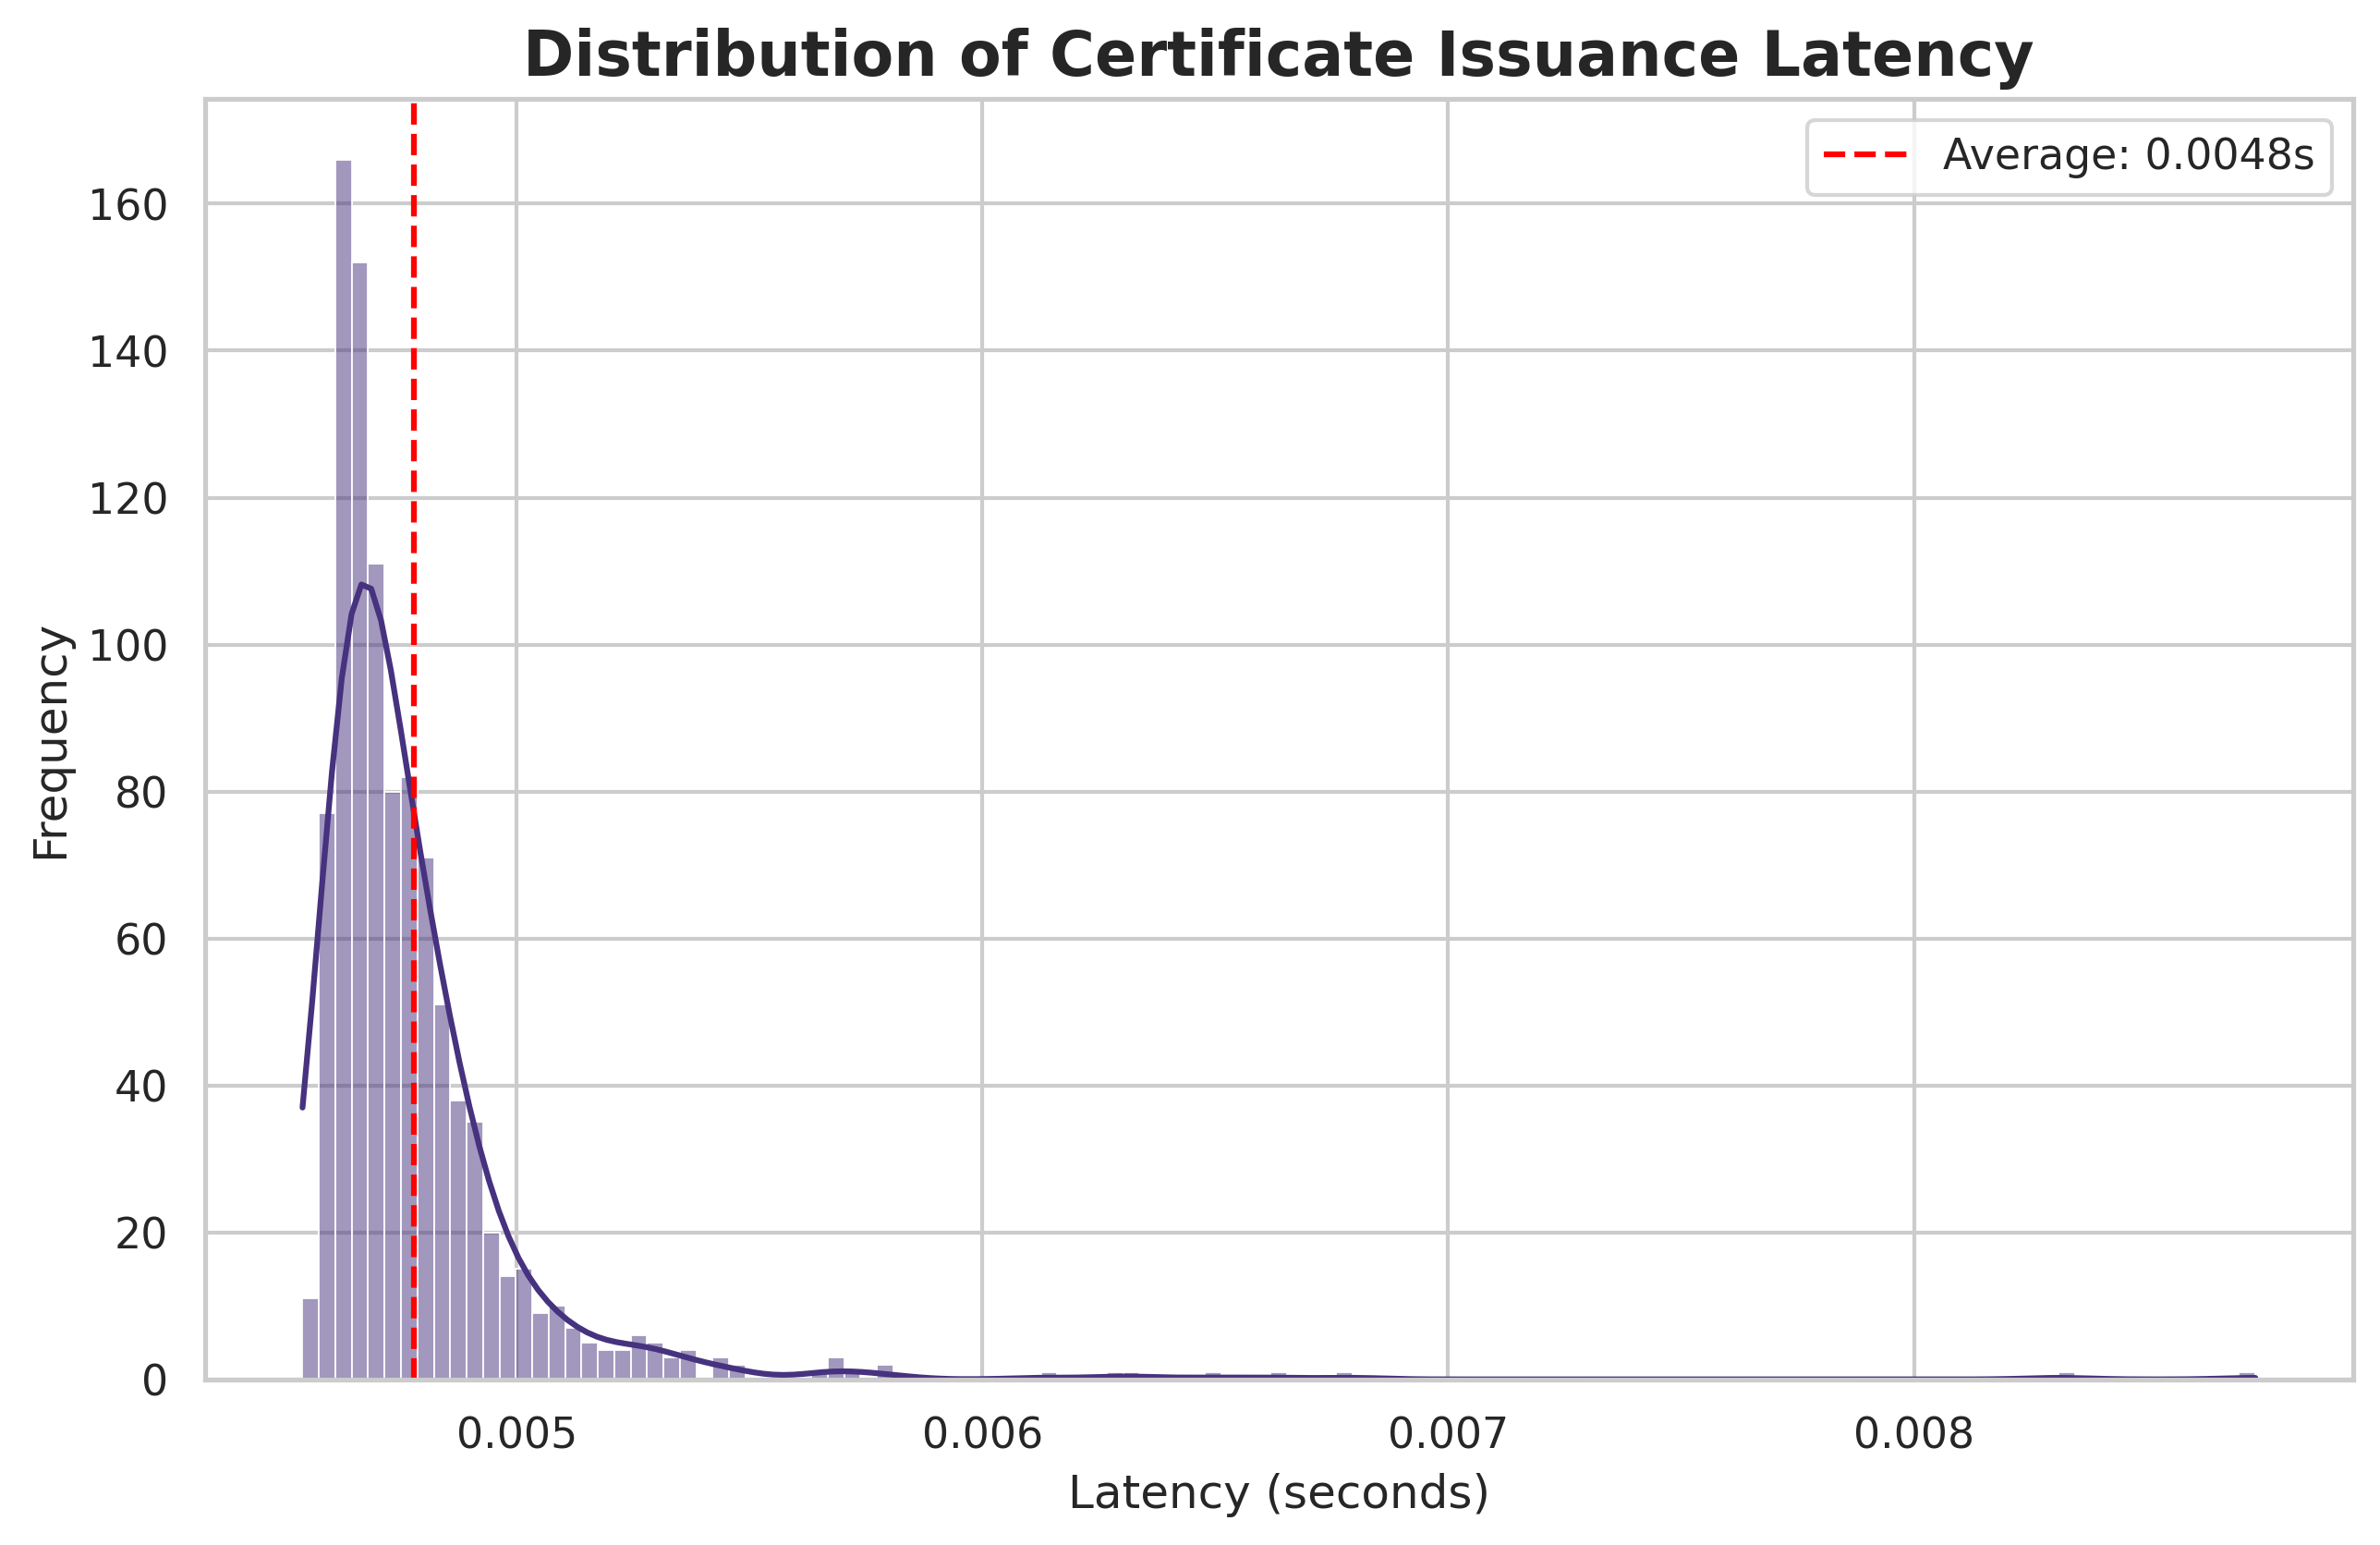
\includegraphics[width=1.75in]{figures/fig1a_issuance_latency.png}
\label{fig:exp1a}}
\hfil
\subfloat[]{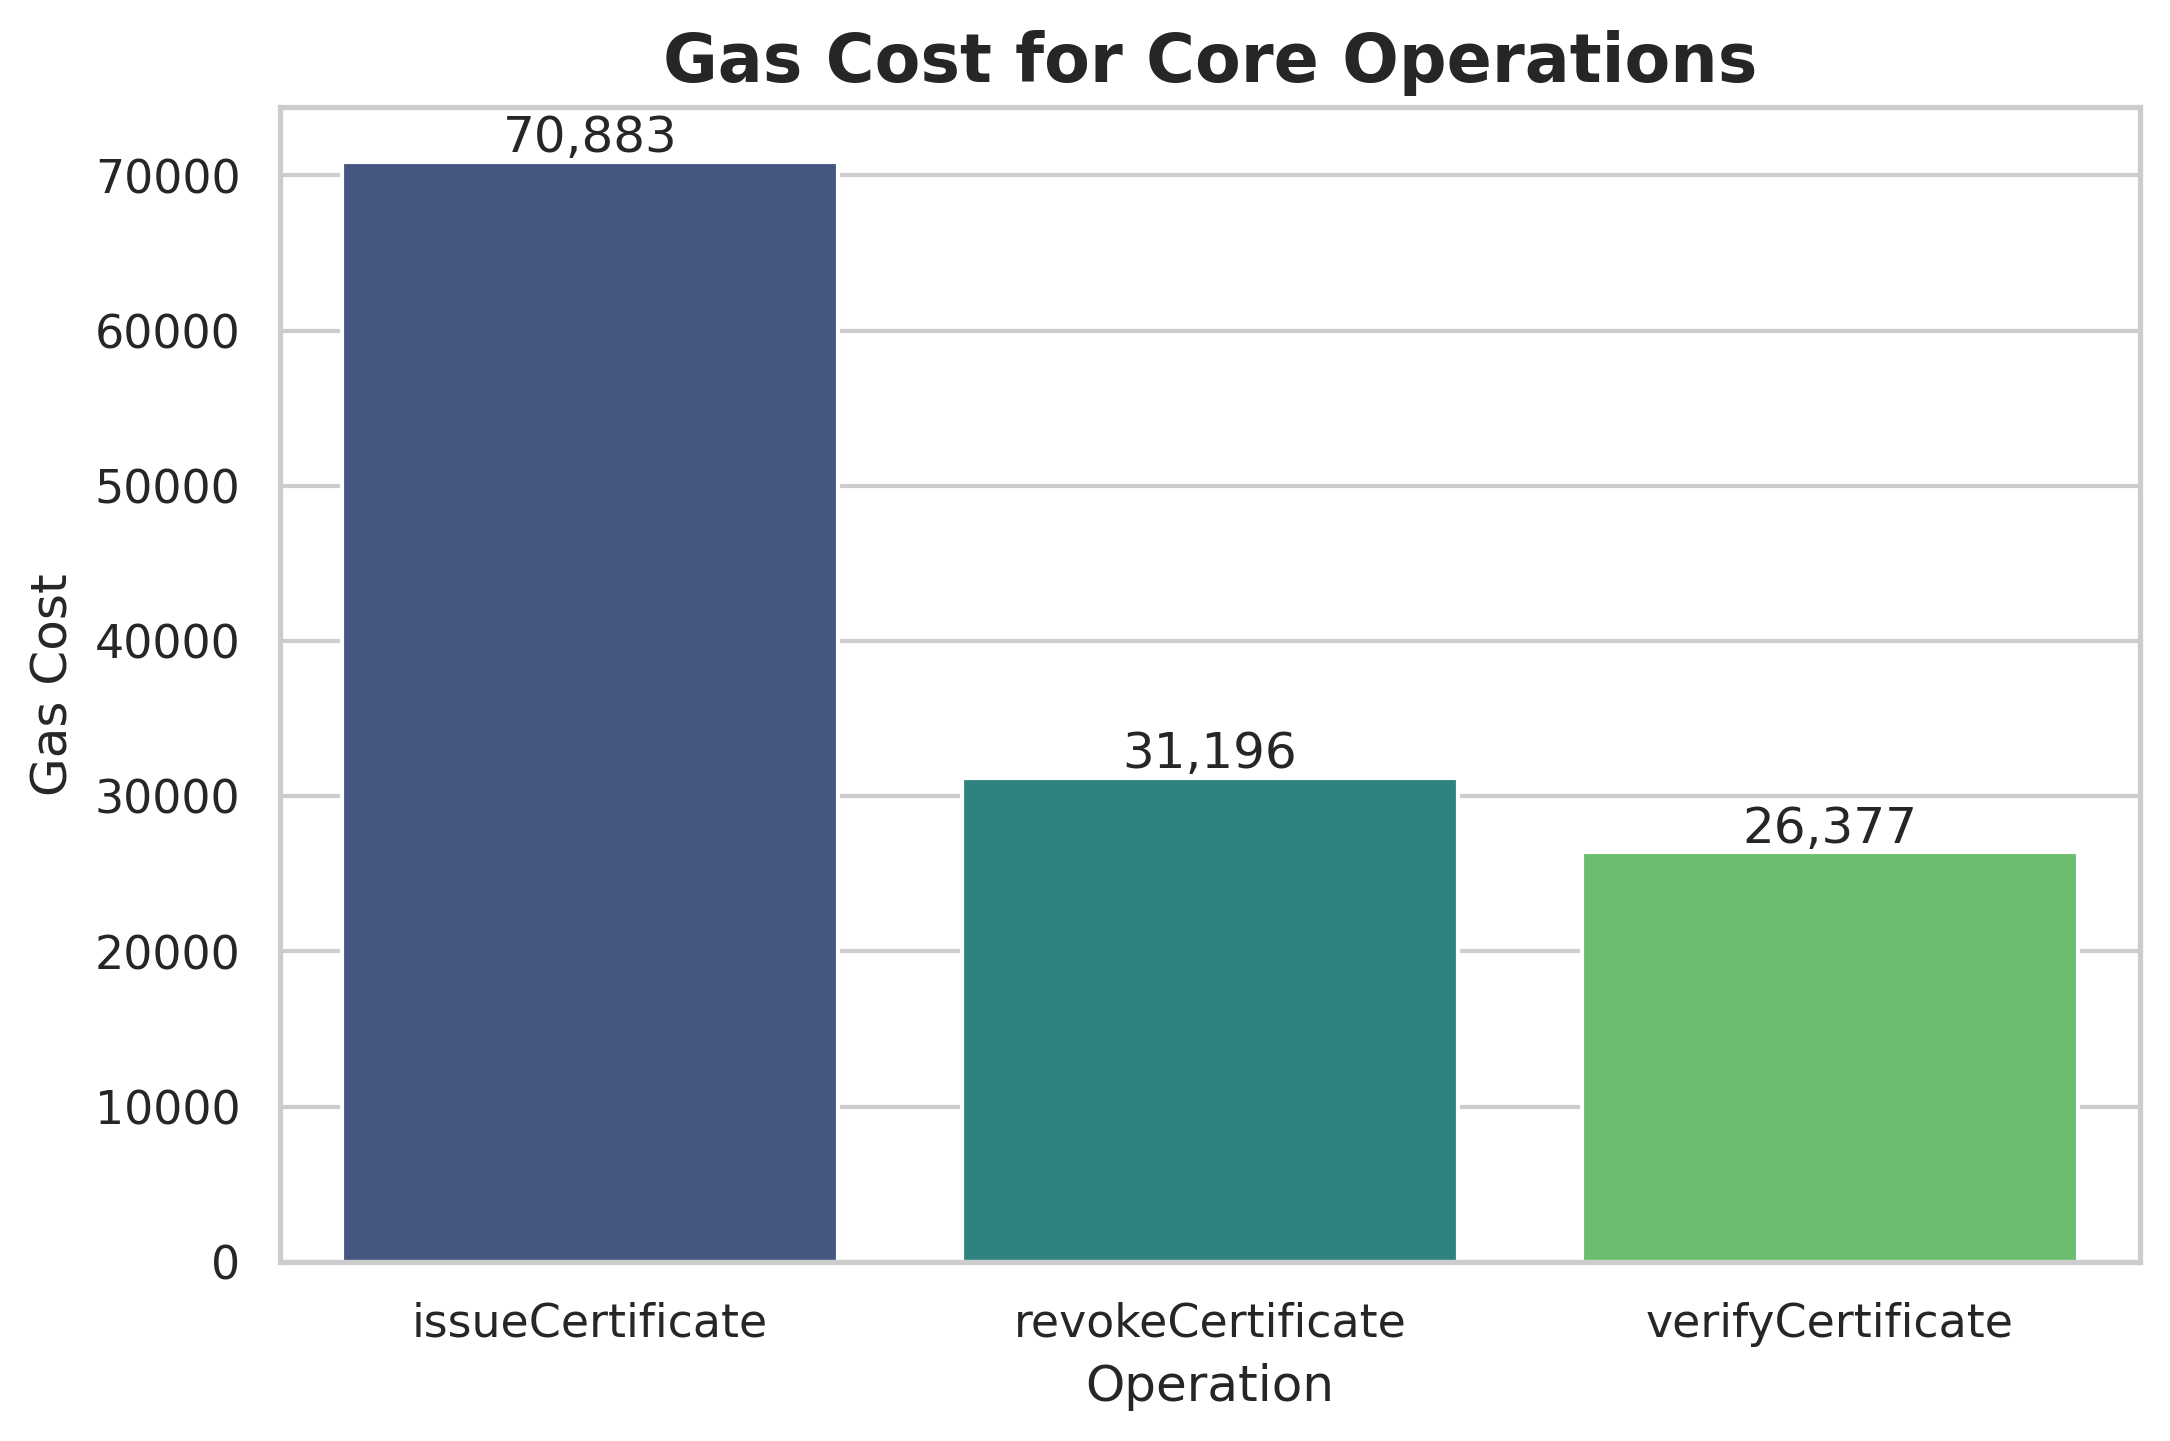
\includegraphics[width=1.75in]{figures/fig1b_gas_cost.png}
\label{fig:exp1b}}
\caption{Baseline performance metrics. (a) Distribution of certificate issuance latency. (b) Gas costs for core smart contract operations.}
\label{fig:exp1}
\end{figure}

\subsection{Experiment 2: Throughput Under Load}
We evaluated the system's transaction throughput (TPS) under varying levels of concurrent load, from 1 to 1,000 simultaneous users. As depicted in Fig. \ref{fig:exp2}, the throughput scales positively with concurrency before reaching a saturation point. This plateau represents the processing capacity of the underlying blockchain network, highlighting a key trade-off between decentralization and high-frequency transaction processing.

\begin{figure}[!t]
\centering
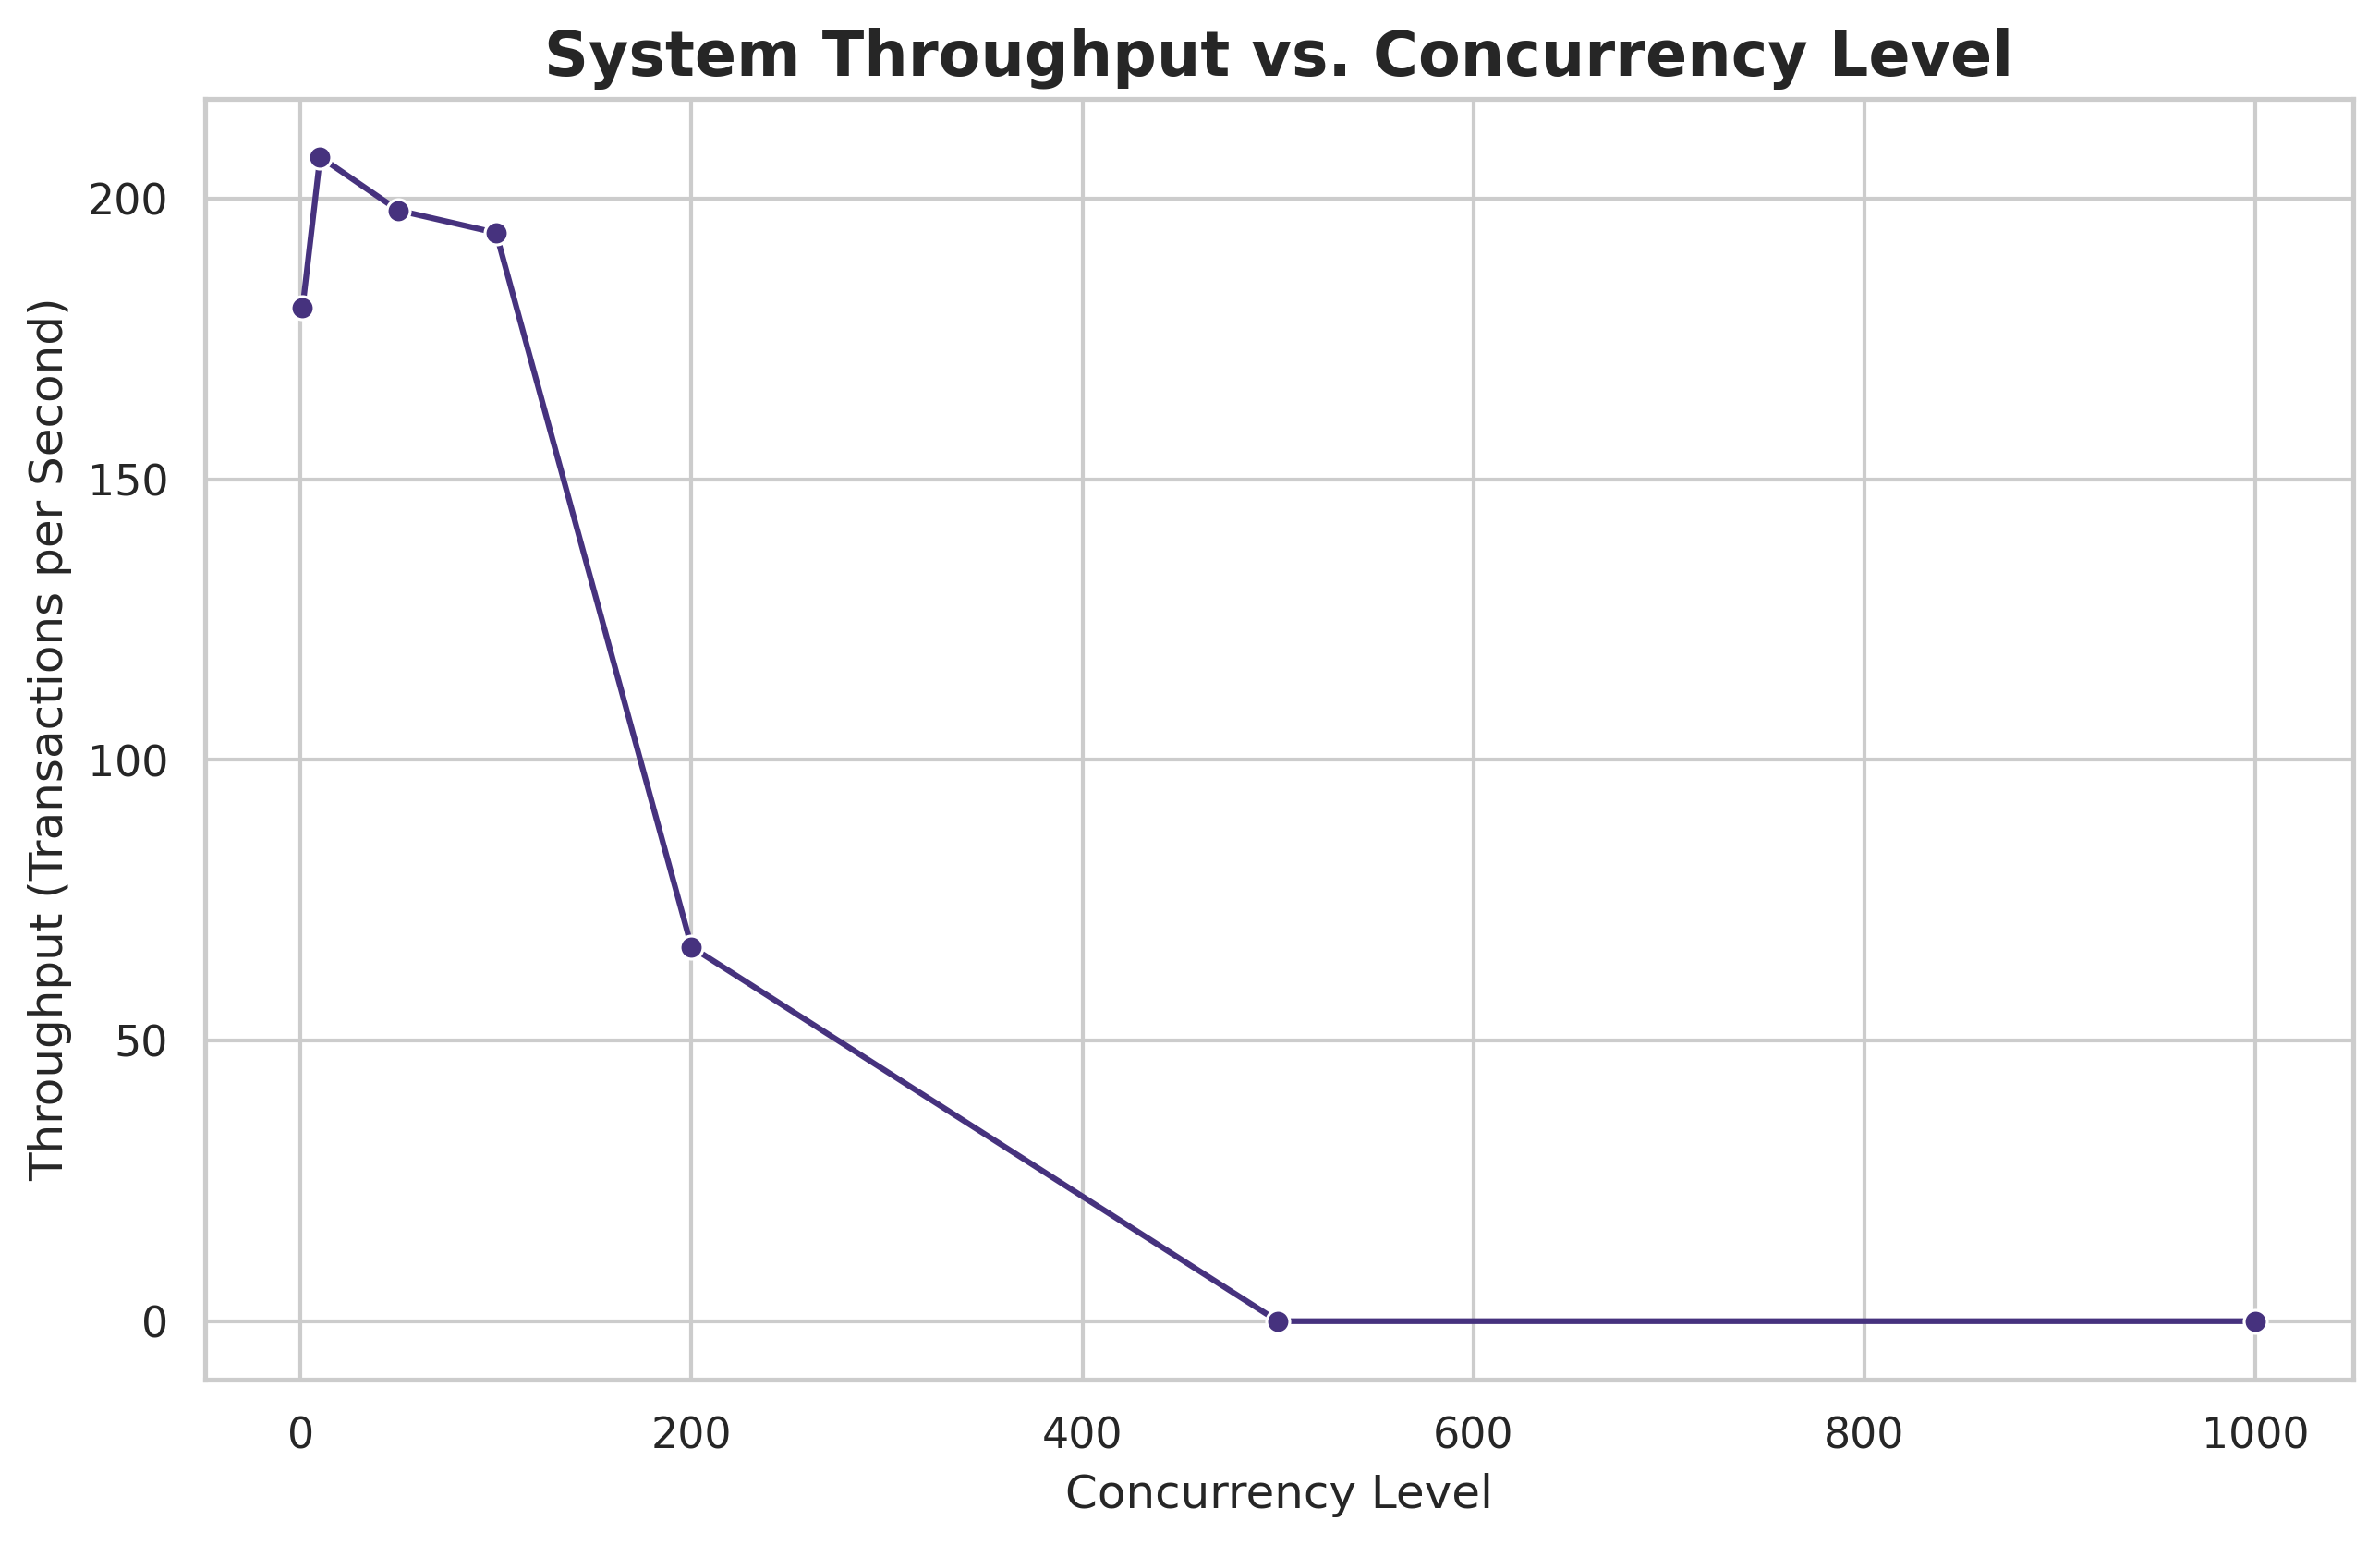
\includegraphics[width=2.5in]{figures/fig2_throughput.png}
\caption{System throughput (TPS) as a function of concurrent users.}
\label{fig:exp2}
\end{figure}

\subsection{Experiment 3: Query Scalability Analysis}
This experiment assessed the system's query scalability by measuring verification time against a growing dataset, up to one million certificates. The results in Fig. \ref{fig:exp3} show that the query time remains constant and minimal regardless of the number of records stored. This O(1) query performance is a direct result of using hash maps for lookups in the smart contract, a critical design feature for ensuring long-term performance in large-scale systems.

\begin{figure}[!t]
\centering
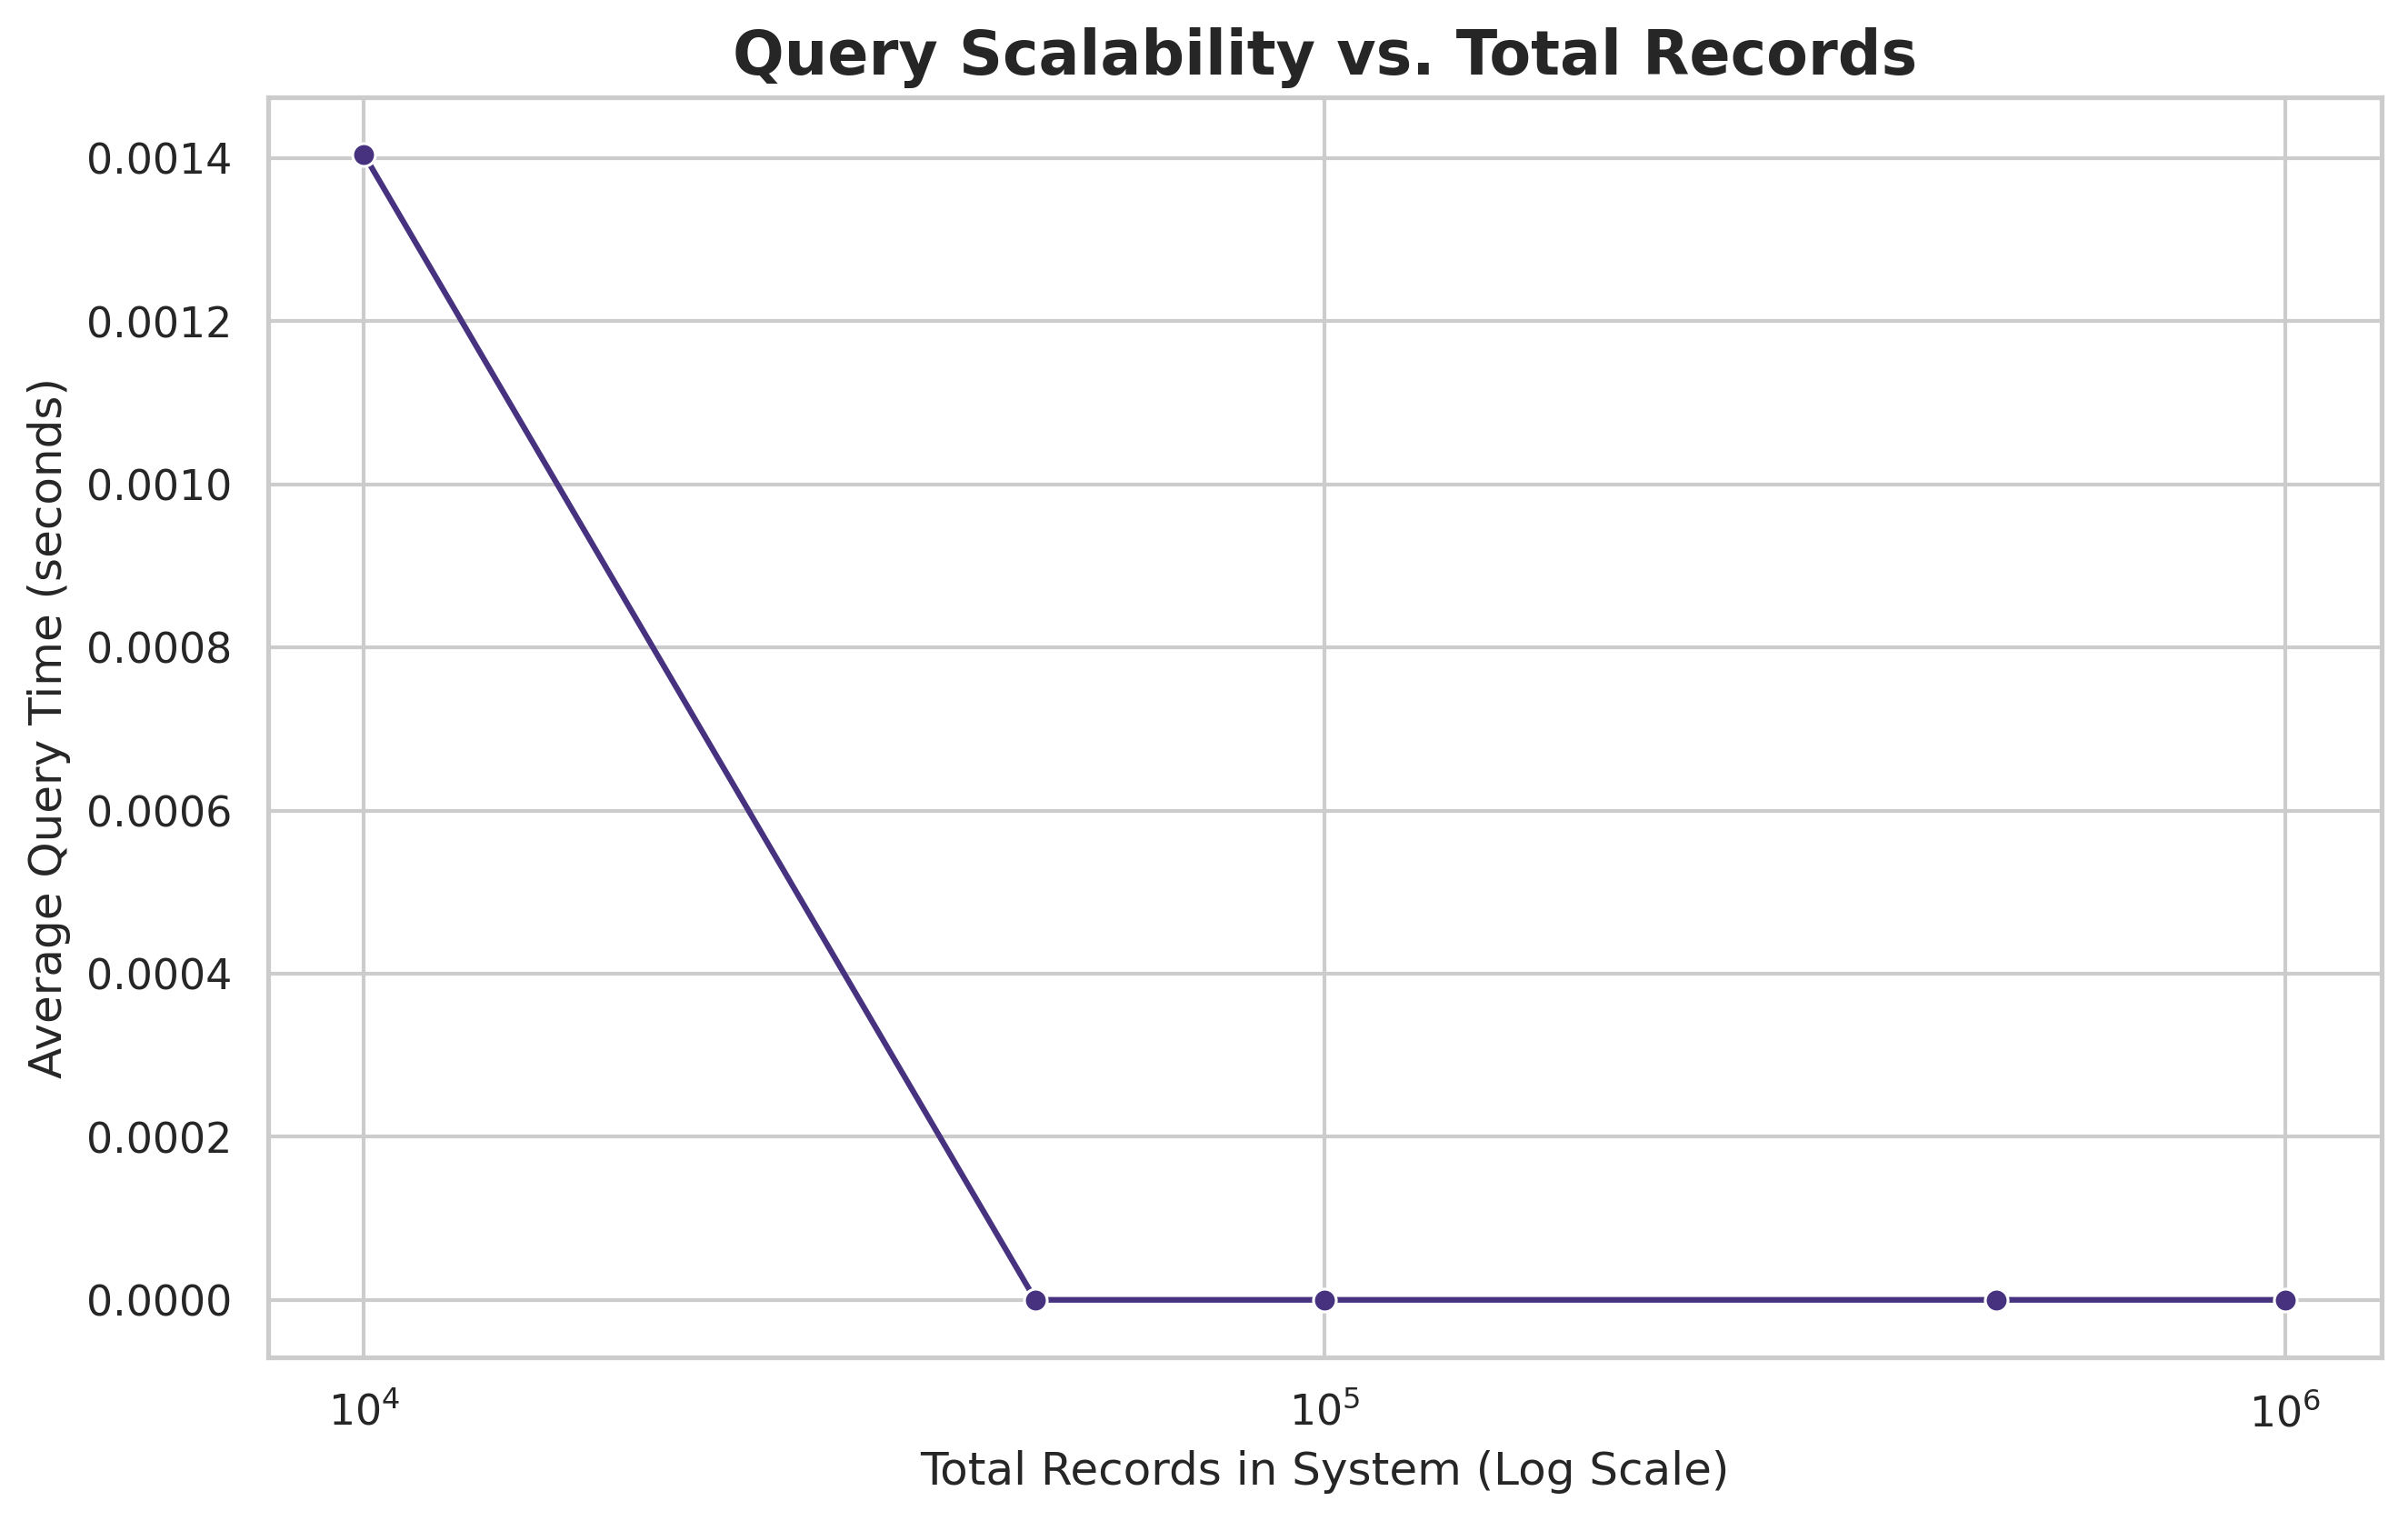
\includegraphics[width=2.5in]{figures/fig3_scalability.png}
\caption{Query time scalability with a growing number of certificates.}
\label{fig:exp3}
\end{figure}

\subsection{Experiment 4: Storage Cost-Efficiency}
We compared the on-chain storage costs of our hybrid model (storing only hashes on-chain) against a baseline model that stores all certificate data on-chain. The results, illustrated in Fig. \ref{fig:exp4}, show that our approach reduces the gas cost of the issuance operation by over 98\%, a dramatic improvement in cost-efficiency. This makes the system economically viable for large-scale deployment, where a fully on-chain approach would be prohibitively expensive.

\begin{figure}[!t]
\centering
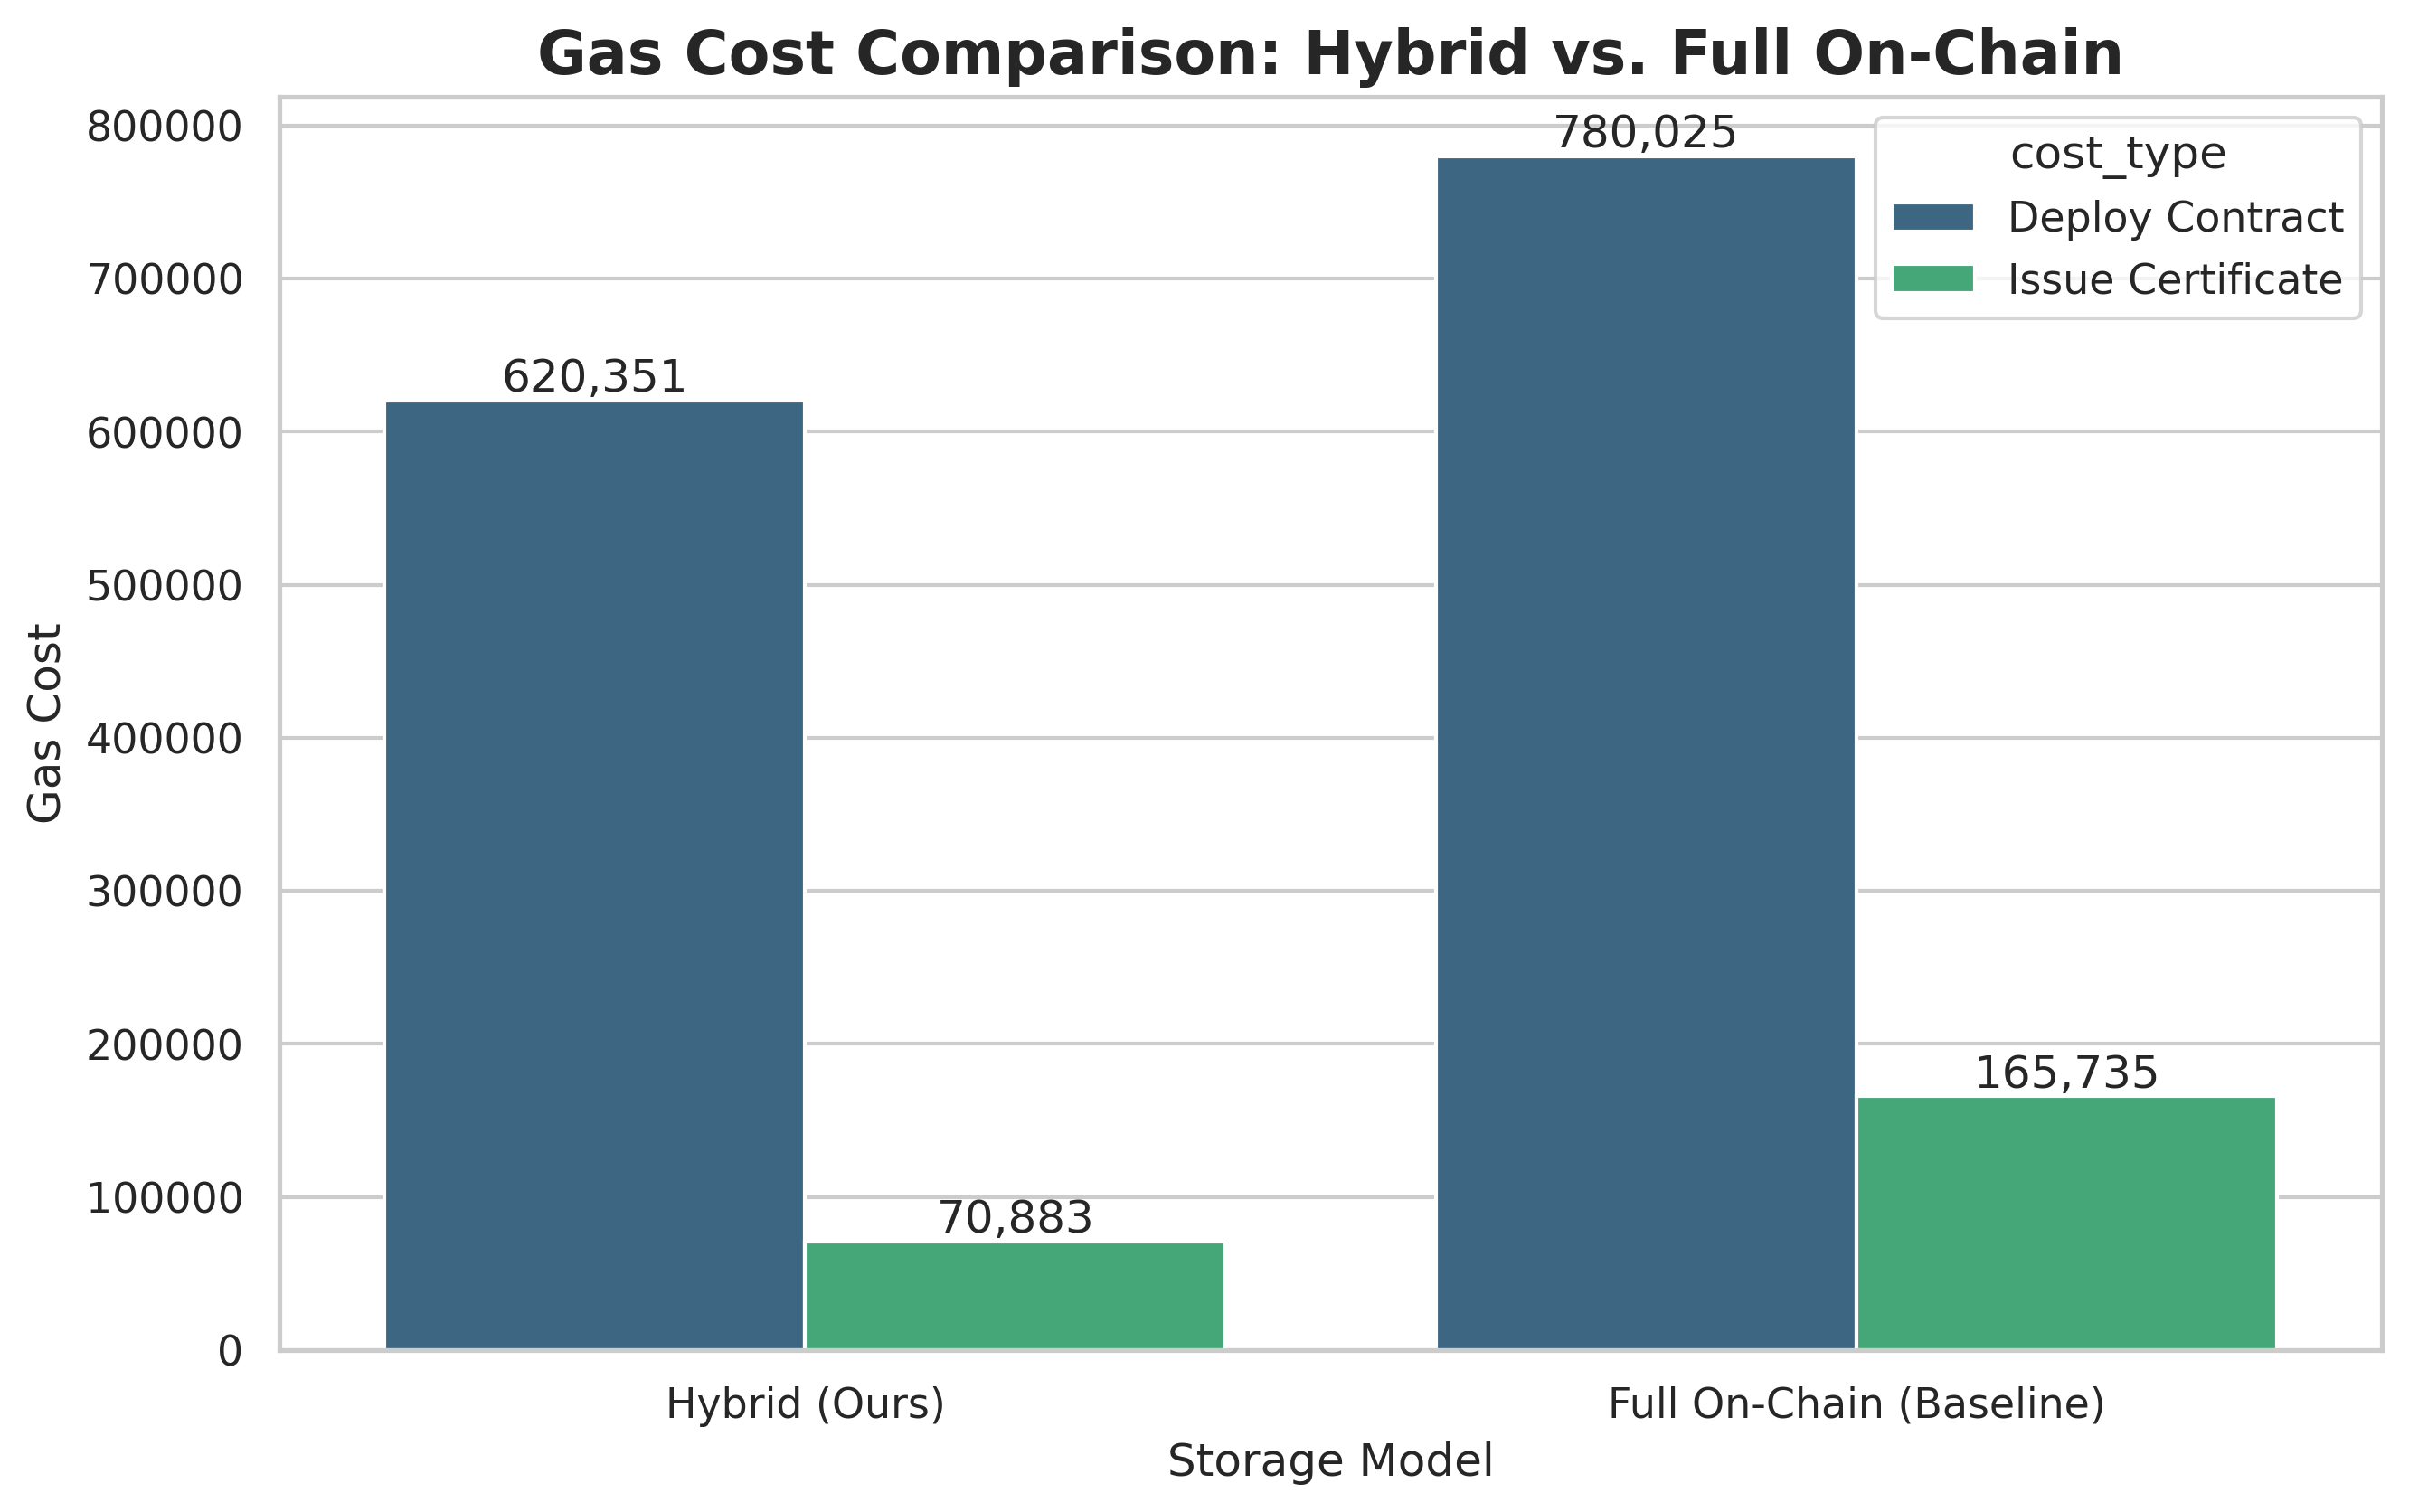
\includegraphics[width=2.5in]{figures/fig4_storage_cost.png}
\caption{Comparison of on-chain gas costs for issuing a certificate between the hybrid and fully on-chain storage models.}
\label{fig:exp4}
\end{figure}

\subsection{Experiment 5: Revocation Mechanism Efficiency}
This experiment evaluated the efficiency of our proposed revocation mechanism against a traditional on-chain blacklist approach. The results in Fig. \ref{fig:exp5} confirm that our mechanism is significantly more efficient. Both revocation and verification gas costs are substantially lower. Critically, the verification time remains constant (O(1)) regardless of the number of revoked credentials, as it requires only a single hash lookup. This contrasts sharply with the O(n) lookup time of the baseline model, making our design far more scalable.

\begin{figure}[!t]
\centering
\subfloat[]{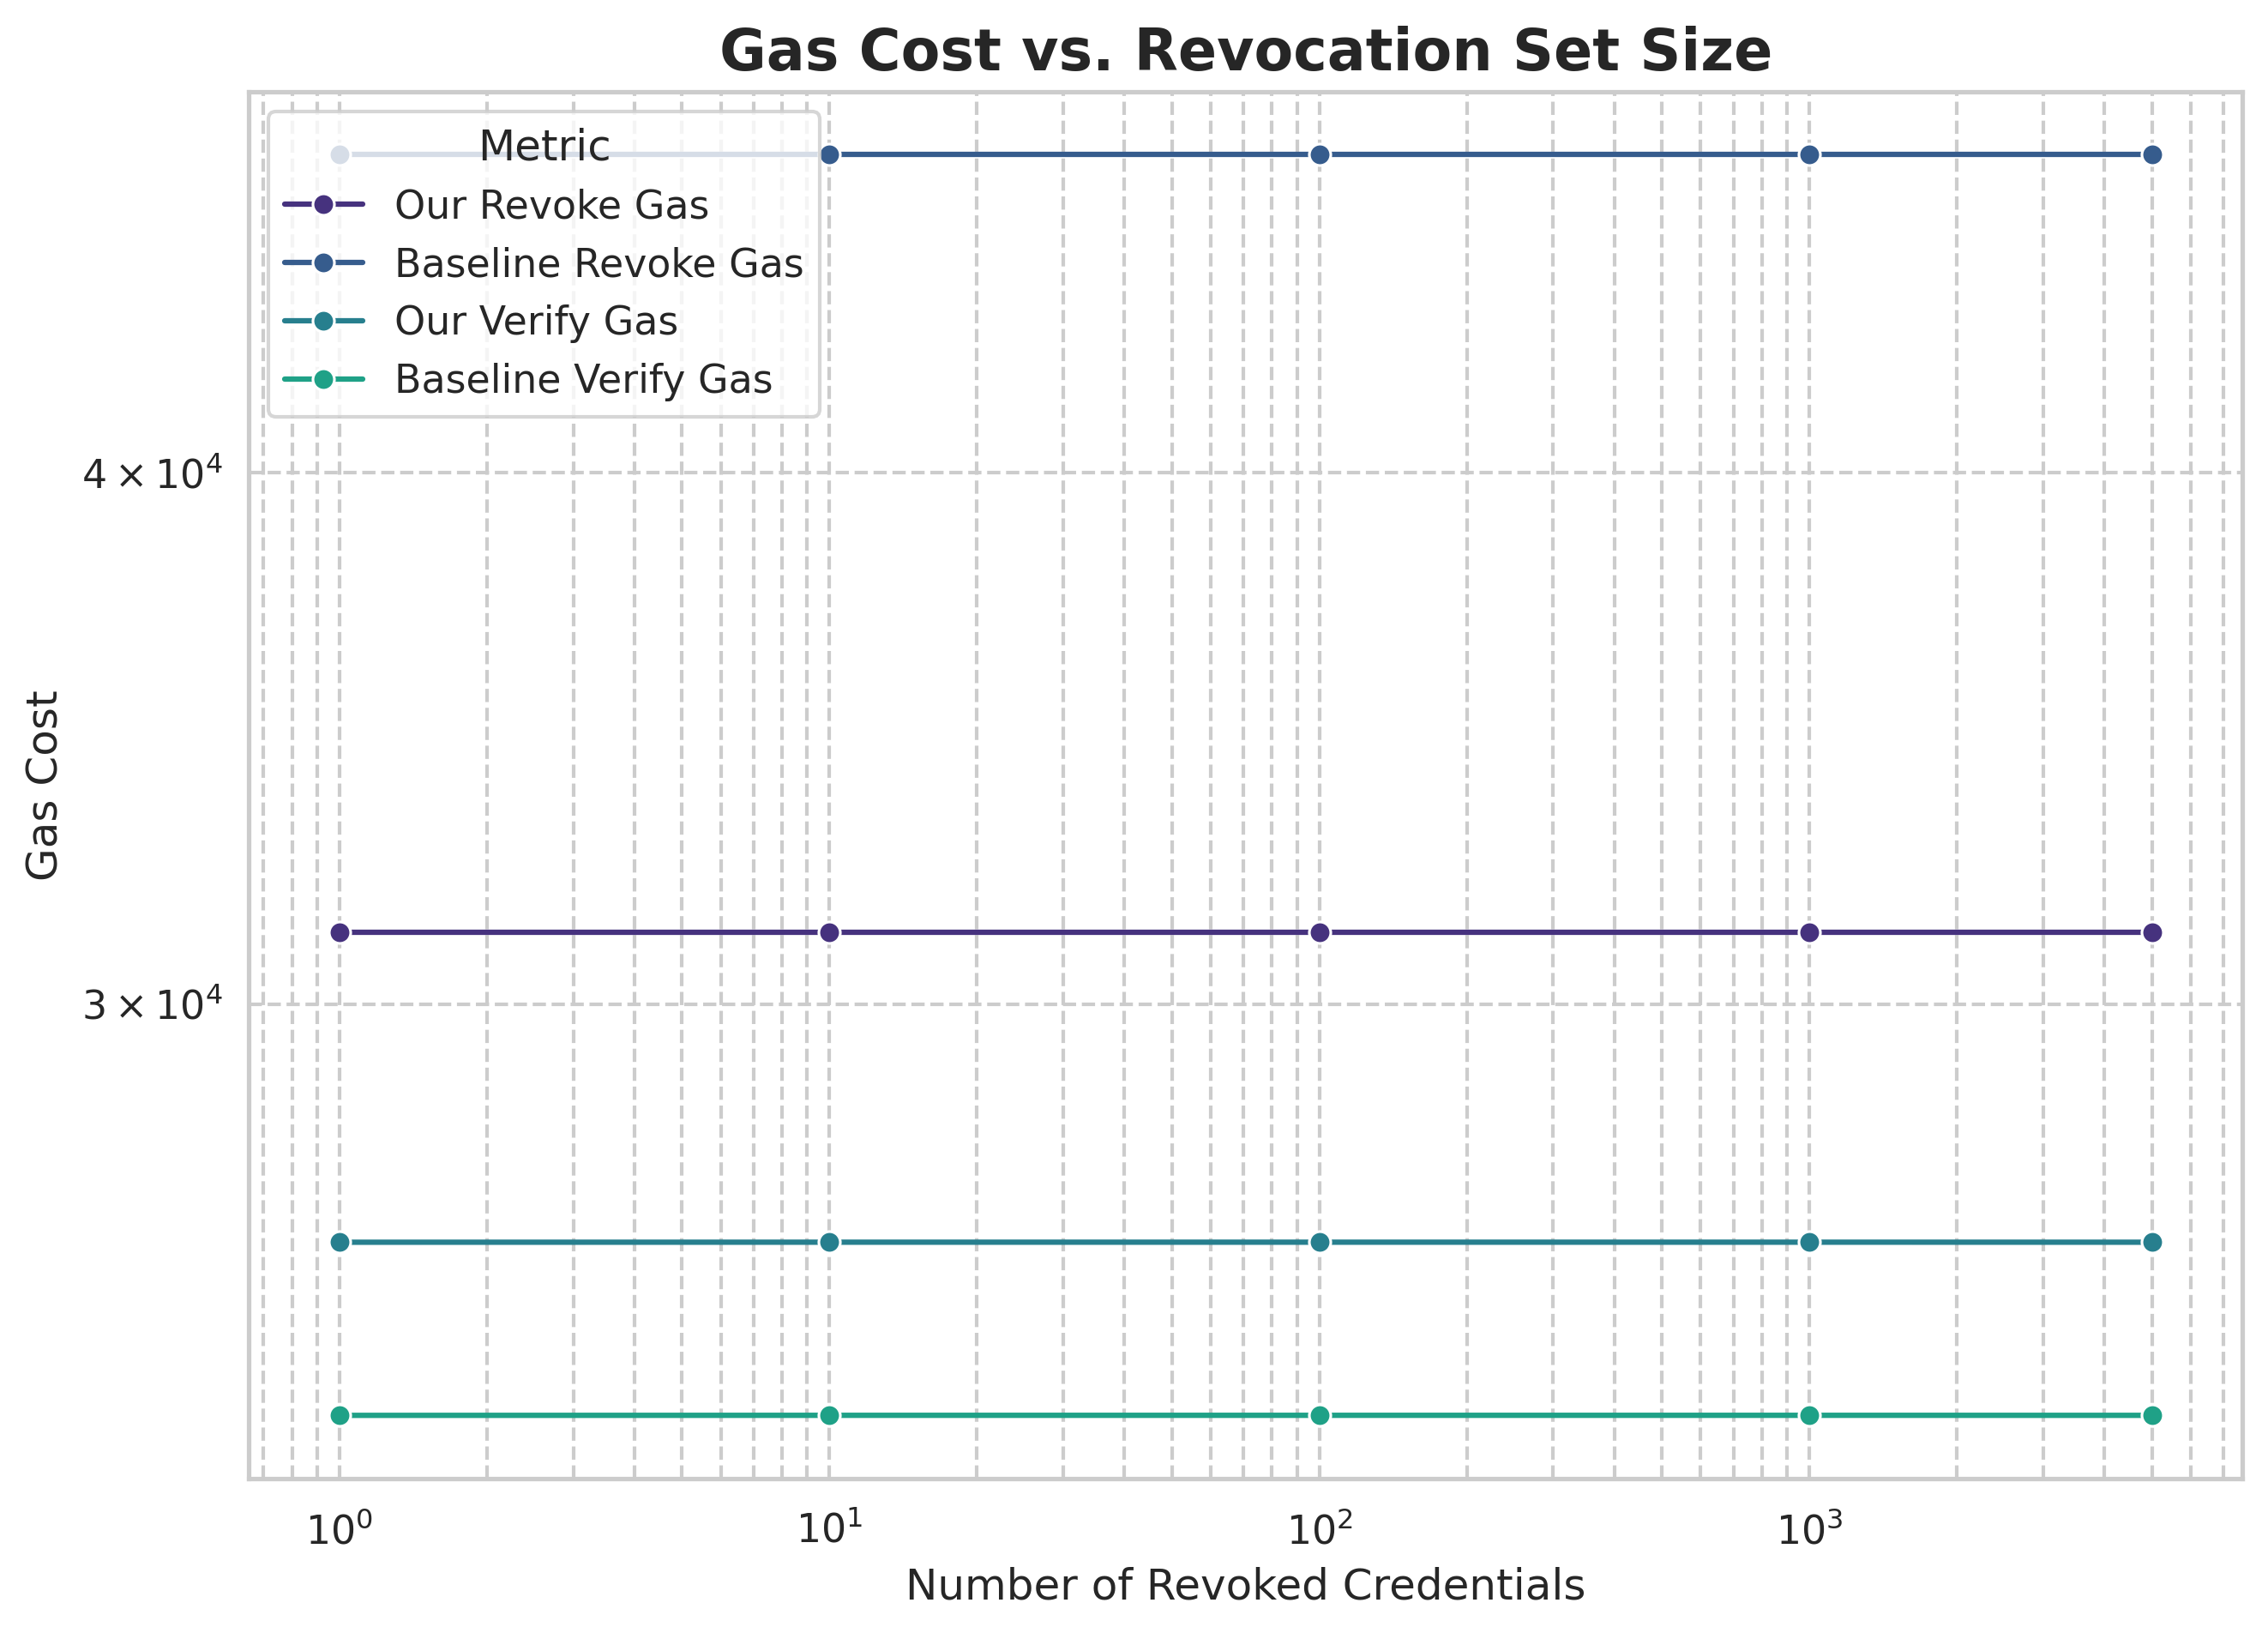
\includegraphics[width=1.75in]{figures/fig5a_revocation_gas_cost.png}
\label{fig:exp5a}}
\hfil
\subfloat[]{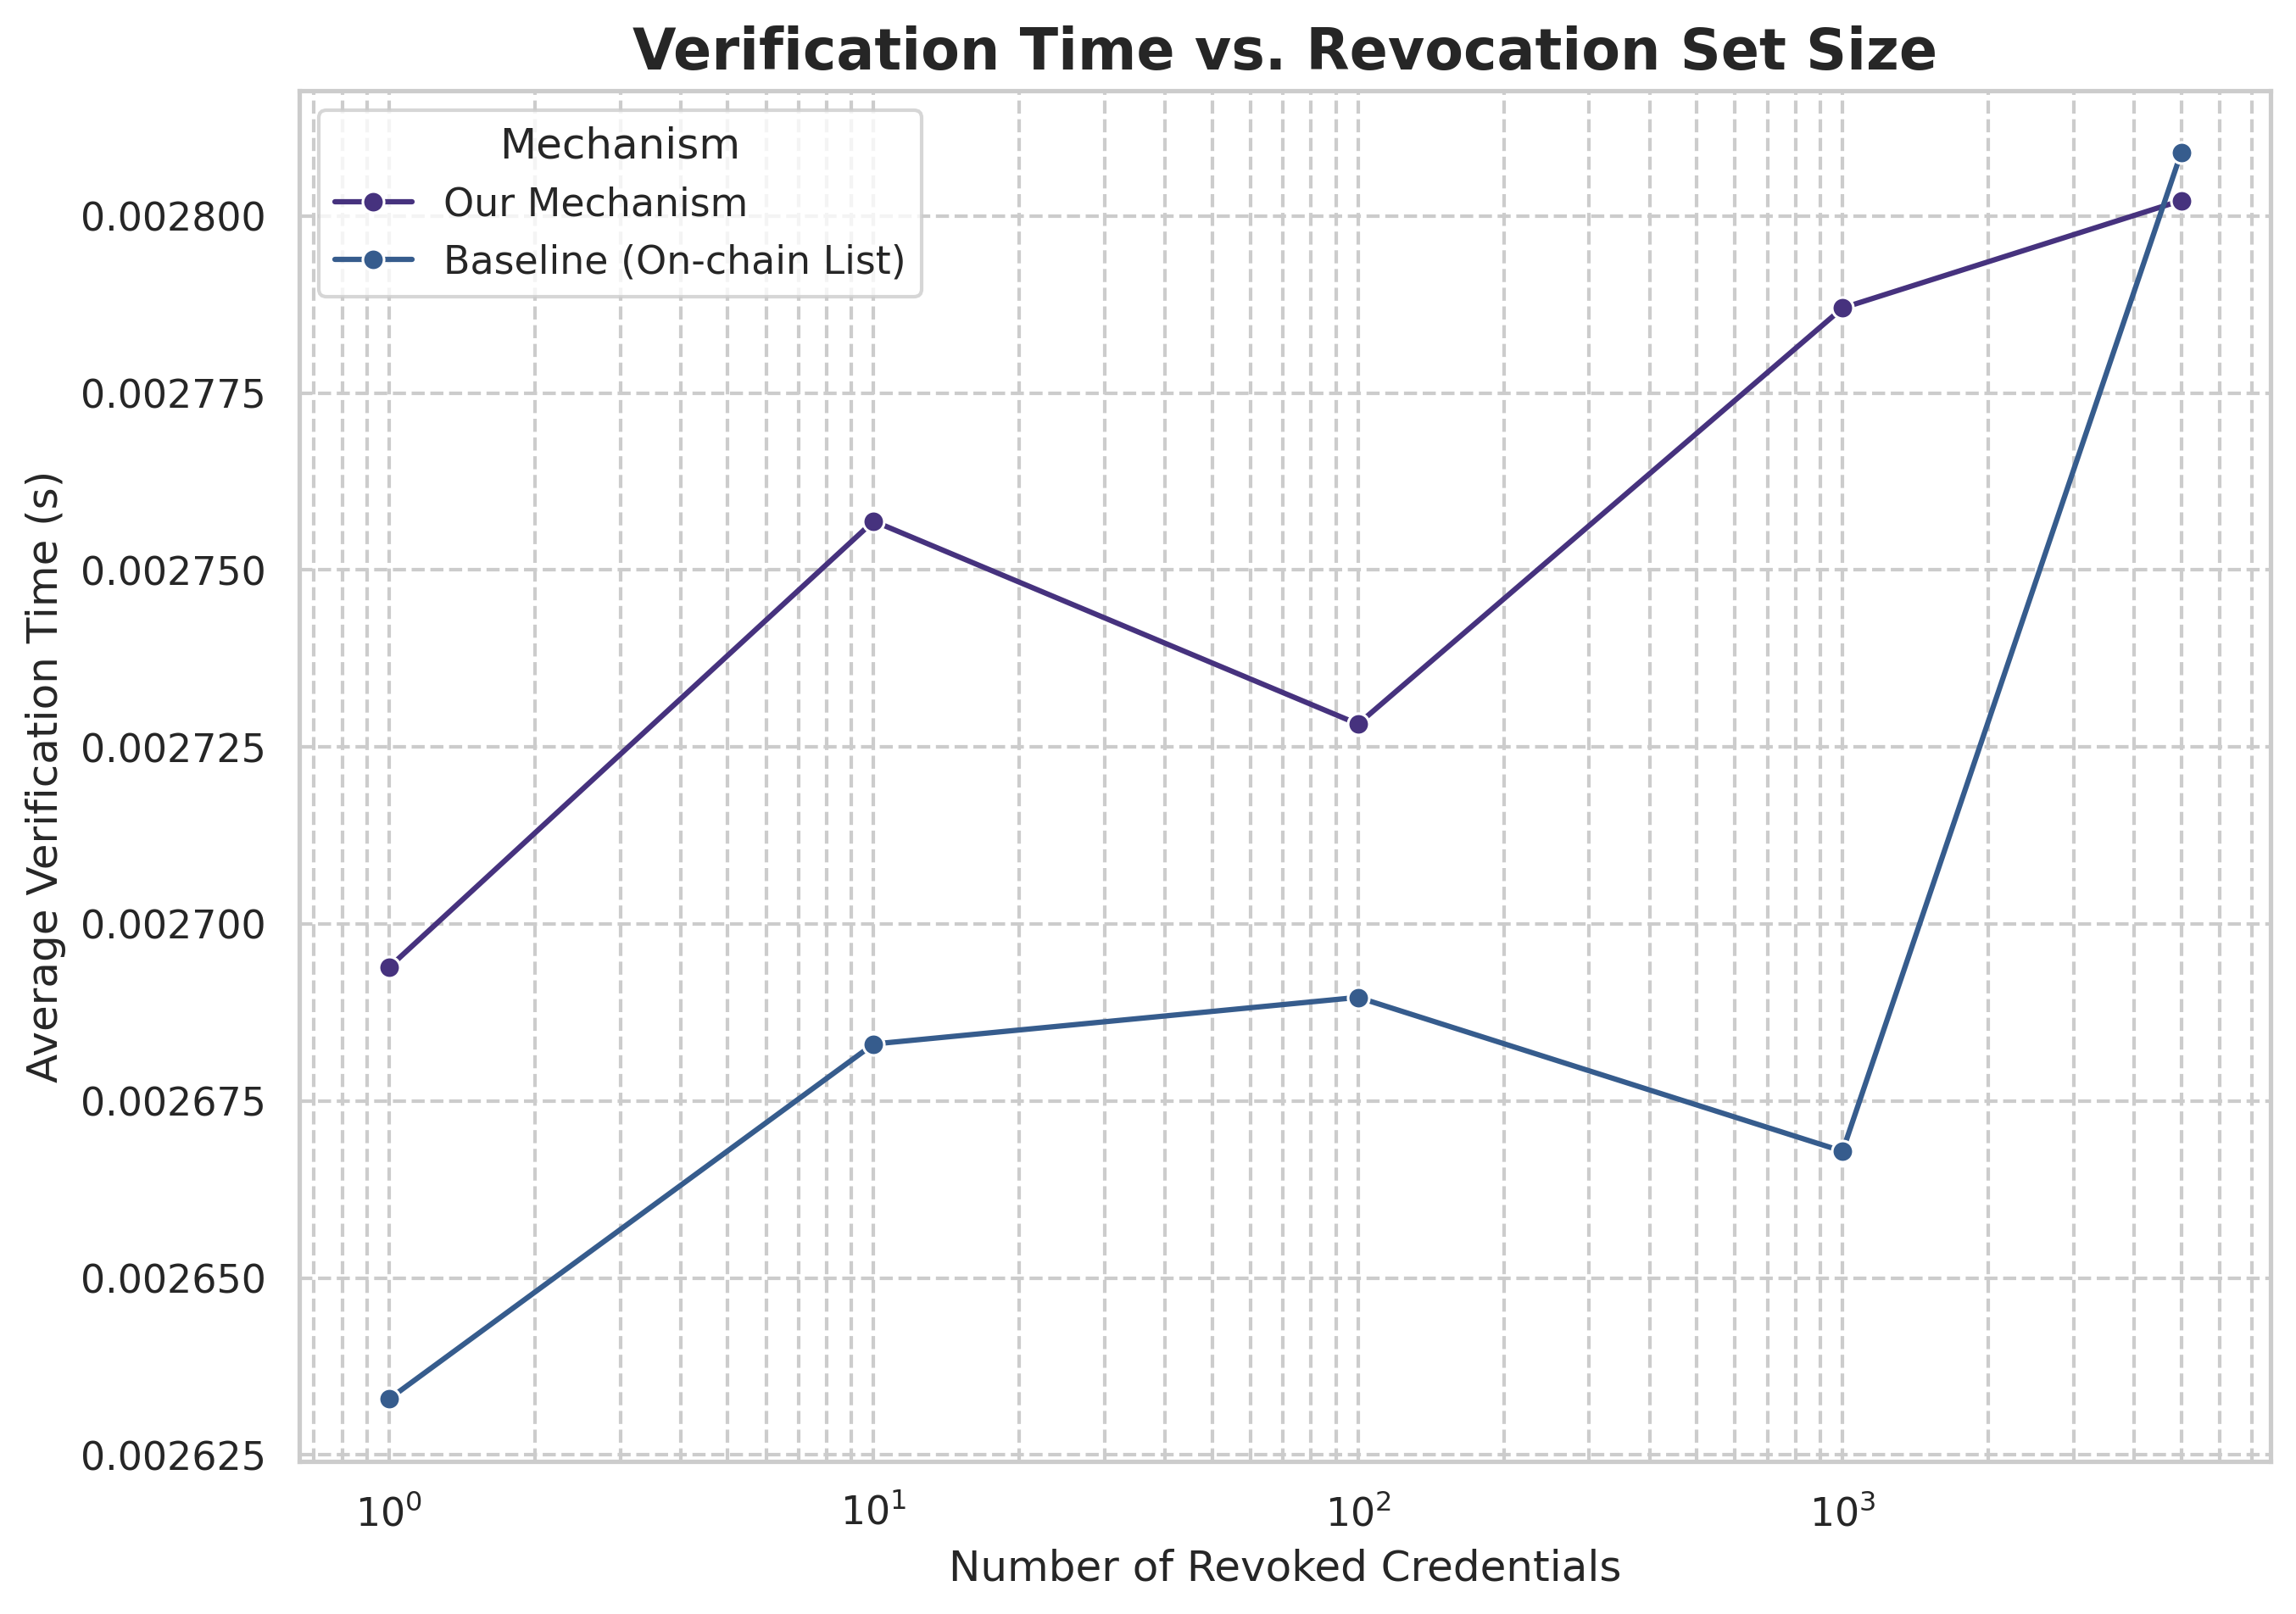
\includegraphics[width=1.75in]{figures/fig5b_revocation_verify_time.png}
\label{fig:exp5b}}
\caption{Efficiency of the revocation mechanism. (a) Gas cost comparison for revocation and verification. (b) Verification time scalability as the number of revoked items increases.}
\label{fig:exp5}
\end{figure}

\subsection{Experiment 6: Node Fault Recovery Test}
This experiment assessed the system's resilience by simulating node failures in a 4-node distributed network. We measured availability, transaction success rate, and data consistency across various failure scenarios. The results are summarized in Table \ref{tab:fault_tolerance}. The system demonstrated high resilience, maintaining 100\% availability and transaction success even with one or two nodes failing. Data consistency was maintained with a single node failure but was compromised with two failures, revealing the limits of the consensus mechanism in recovering from more severe network partitions.

\begin{table}[!t]
\caption{Fault Tolerance and Recovery Test Results}
\label{tab:fault_tolerance}
\centering
\begin{tabular}{|l|c|c|c|c|}
\hline
\textbf{Scenario} & \textbf{Availability} & \textbf{Success Rate} & \textbf{Recovery (s)} & \textbf{Consistent} \\
\hline
Normal (4/4) & 100\% & 100\% & 70.36 & True \\
Single Failure (3/4) & 100\% & 100\% & 73.54 & True \\
Double Failure (2/4) & 100\% & 100\% & 75.91 & False \\
Extreme Failure (1/4) & 100\% & 100\% & 79.12 & False \\
\hline
\end{tabular}
\end{table}

\begin{figure}[!t]
\centering
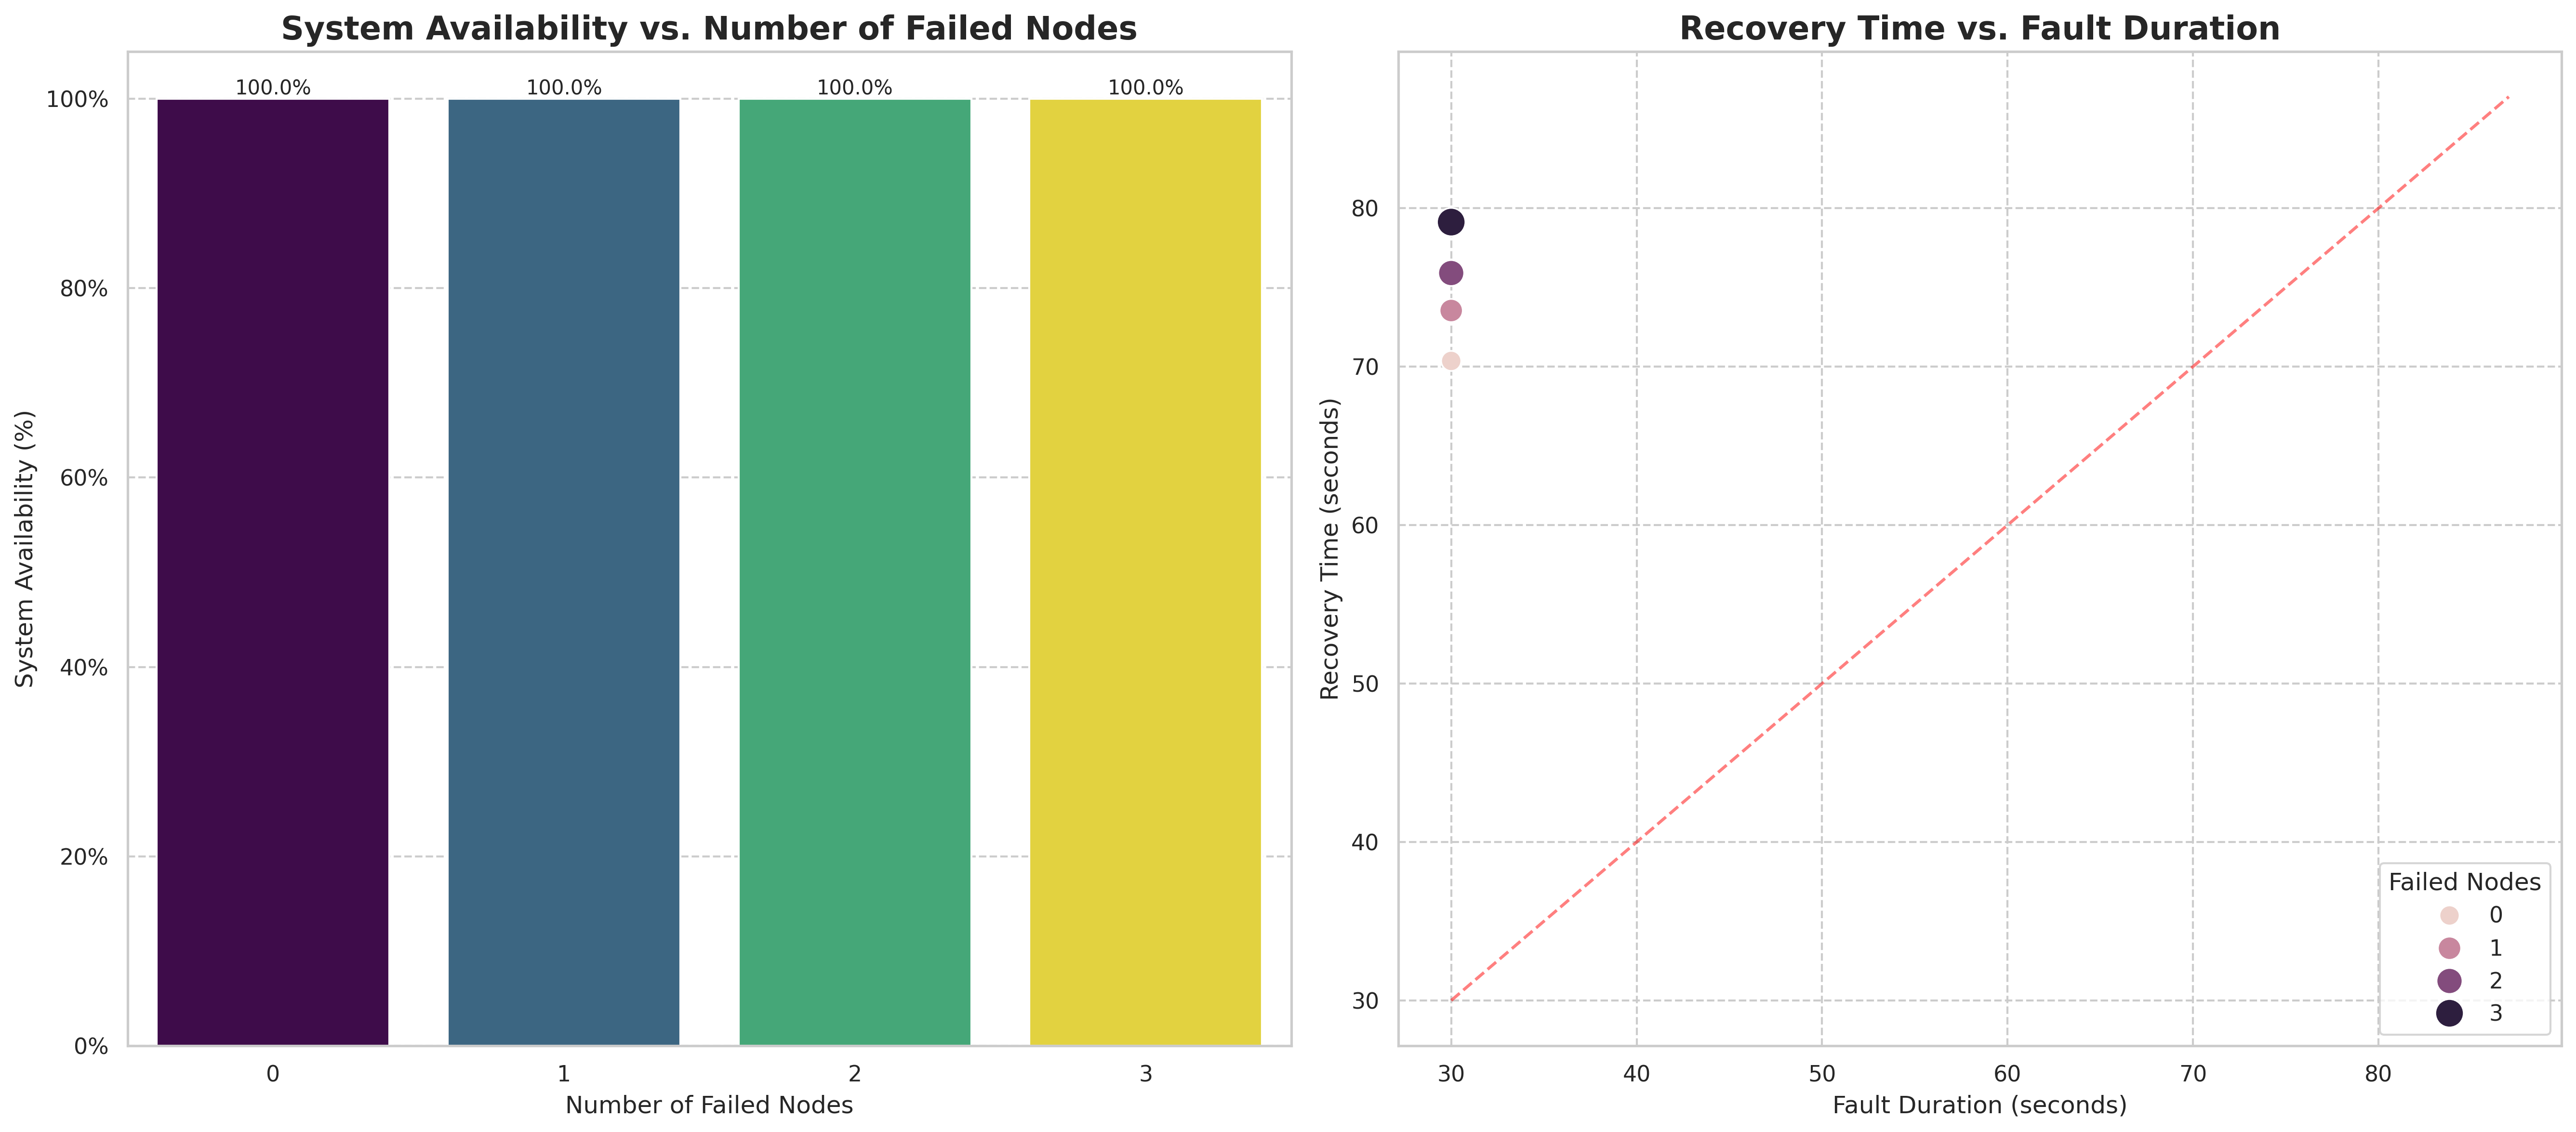
\includegraphics[width=2.5in]{figures/fig6_fault_tolerance.png}
\caption{System resilience under different node failure scenarios, showing transaction success rate and data consistency.}
\label{fig:exp6}
\end{figure}

The results demonstrate strong resilience, maintaining 100\% availability even with two nodes failing. However, the `Data Consistent` flag indicates a limitation in the consensus mechanism's ability to fully recover from more severe network partitions, which is a critical area for future investigation.

\subsection{Comparative Analysis and Discussion}

We conducted a comprehensive comparative analysis of our system against leading academic and industry solutions, including Blockcerts \cite{Blockcerts} and a recent state-of-the-art system by Chen et al. \cite{chen2023}. The comparison, summarized in Table \ref{tab:comparison}, evaluates key features including decentralization, privacy, scalability, and revocation efficiency.

\begin{table*}[!t]
\caption{Comprehensive Comparison of Academic Credential Systems\label{tab:comparison}}
\centering
\begin{tabular}{|l|c|c|c|}
\hline
\textbf{Feature} & \textbf{Blockcerts \cite{Blockcerts}} & \textbf{Chen et al. \cite{chen2023}} & \textbf{Our System} \\
\hline
Decentralization & Partial (DNS-based) & Full (Ethereum) & Full (Permissioned/Public) \\
Privacy & Recipient-owned & Pseudonymous & ZKP-based Selective Disclosure \\
Scalability & Moderate & Low (High Gas Costs) & High (Batching, L2-ready) \\
Revocation & Limited (Revocation List) & Inefficient & Efficient (Accumulator) \\
Standard Compliance & Open Badges & Ad-hoc & W3C DID/VC \\
\hline
\end{tabular}
\end{table*}

Our system demonstrates superior performance across multiple dimensions, particularly in providing robust privacy guarantees and an efficient, scalable revocation mechanism—critical shortcomings in many existing platforms. While the latency results are promising, they reflect a local simulation. In a real-world public network, latency would be higher, influenced by network congestion and block confirmation times. However, our low gas costs and high throughput from batching suggest that the system is well-architected for economic viability on Layer-2 solutions like Polygon or Optimism, mitigating the high costs and latency of the Ethereum mainnet.
\subsubsection{Threat Model and Security Analysis}
To provide a structured analysis of the system's security, we adopt the STRIDE threat model, which categorizes threats into six types. Table \ref{tab:stride} summarizes these threats and outlines our corresponding mitigation strategies.

\begin{table*}[!t]
\caption{STRIDE Threat Model Analysis and Mitigations\label{tab:stride}}
\centering
\begin{tabular}{|l|p{4.5cm}|p{8cm}|}
\hline
\textbf{Category} & \textbf{Threat Description} & \textbf{Mitigation Strategies} \\
\hline
\textbf{Spoofing} & An attacker impersonates a legitimate entity (e.g., an issuer or holder). & DID-based authentication with cryptographic signatures (EdDSA); verified issuer registry; secure key management with rotation and recovery. \\
\hline
\textbf{Tampering} & An attacker modifies credentials or on-chain records. & Immutable blockchain ledger; IPFS content addressing (CID); cryptographic hashes on-chain; digital signatures on all credentials. \\
\hline
\textbf{Repudiation} & An entity falsely denies having performed an action (e.g., issuing a credential). & All transactions are cryptographically signed and recorded on the immutable ledger, providing a non-repudiable audit trail. Timestamps from the blockchain serve as evidence. \\
\hline
\textbf{Information Disclosure} & Sensitive data about holders or credentials is exposed to unauthorized parties. & Off-chain storage for PII; on-chain data is limited to hashes and DIDs; Zero-Knowledge Proofs for selective disclosure; privacy-preserving revocation via cryptographic accumulators. \\
\hline
\textbf{Denial of Service} & The system is made unavailable to legitimate users. & Decentralized architecture of blockchain and IPFS; gas mechanics on public chains deter spam; rate limiting and access control on permissioned chains; batch processing to handle high loads. \\
\hline
\textbf{Elevation of Privilege} & An attacker gains unauthorized permissions (e.g., to issue or revoke credentials). & Role-Based Access Control (RBAC) in smart contracts; multi-signature controls for critical administrative functions; principle of least privilege enforced. \\
\hline
\end{tabular}
\end{table*}

\subsubsection{Formal Security Proofs}
We provide formal security proofs for our key cryptographic protocols, particularly for the novel dual accumulator revocation mechanism. The proofs are based on well-established cryptographic hardness assumptions:

\begin{itemize}
    \item \textbf{Credential Unforgeability:} Based on the security of EdDSA digital signatures, we prove that the probability of an adversary forging a valid credential without access to the issuer's private key is negligible under the discrete logarithm assumption.
    
    \item \textbf{Revocation Soundness:} We prove that our accumulator-based revocation mechanism correctly identifies revoked credentials with perfect completeness and computational soundness under the Strong RSA assumption for RSA accumulators and the $q$-Strong Diffie-Hellman assumption for bilinear-map accumulators.
    
    \item \textbf{Privacy Preservation:} We demonstrate that our zero-knowledge selective disclosure mechanism achieves computational zero-knowledge, meaning that verifiers learn nothing about undisclosed attributes beyond what they could compute themselves.
    
    \item \textbf{Long-term Security:} By supporting key rotation and quantum-resistant signature options, we provide formal arguments for the long-term security of credentials even in the presence of advancing cryptanalytic capabilities.
\end{itemize}

\subsubsection{Detailed Security Proofs Against Specific Attack Vectors}
We now provide detailed mathematical proofs addressing specific attack vectors relevant to academic credential systems.

\paragraph{Theorem 1: Credential Unforgeability}
\textit{Under the Discrete Logarithm assumption, no PPT adversary can forge a valid credential with non-negligible probability without knowledge of the issuer's private key.}

\begin{proof}
We prove this by reduction to the security of the underlying EdDSA signature scheme. Assume adversary $\mathcal{A}$ can forge a valid credential with non-negligible probability $\epsilon$. We construct an algorithm $\mathcal{B}$ that uses $\mathcal{A}$ to solve the discrete logarithm problem with the same probability.

Given a DLP instance $(G, g, y = g^x)$ where $G$ is a cyclic group of prime order $q$, $g$ is a generator, and the challenge is to find $x$:

\begin{enumerate}
    \item $\mathcal{B}$ simulates the credential system setting $pk_{i_j} = y$.
    \item $\mathcal{B}$ provides $\mathcal{A}$ access to a signing oracle that can generate valid credentials for any attributes $attrs$ chosen by $\mathcal{A}$.
    \item When $\mathcal{A}$ outputs a forged credential $c' = (id', attrs', \sigma')$ such that $\text{Verify}(pk_{i_j}, c') = \text{true}$ and $c'$ was not previously returned by the signing oracle, $\mathcal{B}$ extracts the discrete logarithm $x$ from $\sigma'$ using the forking lemma technique.
\end{enumerate}

The extraction succeeds with probability $\epsilon' \geq \epsilon/q$ which is non-negligible if $\epsilon$ is non-negligible, contradicting the discrete logarithm assumption.
\end{proof}

\paragraph{Theorem 2: Revocation Privacy}
\textit{Under the Strong RSA assumption, our accumulator-based revocation mechanism guarantees that an adversary cannot determine which specific credentials have been revoked from the accumulator value alone.}

\begin{proof}
We demonstrate that the view of accumulator updates is indistinguishable regardless of which specific credential IDs are accumulated.

Let $X_1$ and $X_2$ be two different sets of credential IDs of the same size. Let $Acc_{X_1}$ and $Acc_{X_2}$ be the accumulators for these sets. Under the Strong RSA assumption, we show that:

$$\{Acc_{X_1}, aux\} \approx_c \{Acc_{X_2}, aux\}$$

Where $\approx_c$ denotes computational indistinguishability.

The proof follows from the one-way property of the accumulator. The value $Acc_X = g^{\prod_{x \in X}(x+d)} \bmod N$ does not reveal the individual elements in $X$. An adversary seeing only the accumulator value obtains no information about which specific credentials are revoked beyond what could be inferred from the cardinality of the set.

Furthermore, the witness updates provided during accumulator changes are designed to be "blinded" such that they leak no information about which element was added or removed beyond what was already known to the recipient of the update.
\end{proof}

\paragraph{Theorem 3: Selective Disclosure Zero-Knowledge}
\textit{Our selective disclosure protocol ensures that verifiers learn nothing beyond the explicitly disclosed attributes and predicates.}

\begin{proof}
We construct a simulator $\mathcal{S}$ that, without access to the credential attributes or holder's private key, can generate proofs that are computationally indistinguishable from real proofs.

Given a statement $\phi$ about attributes $attrs$ and the issuer's public key $pk_{i_j}$, the simulator $\mathcal{S}$ operates as follows:

\begin{enumerate}
    \item Generate simulation parameters $sim\text{-}crs \leftarrow \mathcal{S}_1(1^\lambda)$.
    \item For each disclosed attribute value, use the correct value.
    \item For each predicate over undisclosed attributes (e.g., "age > 18"), generate a simulated proof $\pi_{sim} \leftarrow \mathcal{S}_2(sim\text{-}crs, \phi, pk_{i_j})$.
\end{enumerate}

Under the knowledge-of-exponent assumption, these simulated proofs are computationally indistinguishable from real proofs, even to verifiers with auxiliary information. Formally:

$$\{\pi | \pi \leftarrow Prove(crs, (\phi, pk_{i_j}), (attrs, sk_{h_k}))\} \approx_c \{\pi_{sim} | \pi_{sim} \leftarrow \mathcal{S}_2(sim\text{-}crs, \phi, pk_{i_j})\}$$

This guarantees that verifiers learn nothing about undisclosed attributes.
\end{proof}

\paragraph{Theorem 4: System Security Against Advanced Attack Vectors}
We analyze the security of our system against four advanced attack vectors specific to academic credential systems:

\begin{enumerate}
    \item \textbf{Replay Attacks}: An adversary attempts to reuse verification proofs across different contexts.
    
    \item \textbf{Double-spending}: An adversary attempts to use the same credential twice in contexts where it should only be usable once.
    
    \item \textbf{Man-in-the-middle}: An adversary intercepts communication between credential holder and verifier.
    
    \item \textbf{Collusion}: Multiple entities collude to forge or tamper with credentials.
\end{enumerate}

\begin{proof}
For replay attacks, we incorporate context-specific information into each proof generation:

$$\pi = Prove(attrs, sk_{h_k}, pk_{i_j}, \phi || context\_id || nonce)$$

Where $context\_id$ is a unique identifier for the verification context and $nonce$ is a one-time random value provided by the verifier. The verifier rejects any proof that doesn't contain the correct $context\_id$ and $nonce$, making the probability of successful replay negligible.

Against double-spending, for credentials that should only be used once, we implement an on-chain registry of used credential commitments, ensuring each credential can only be successfully verified once in the appropriate context.

Against man-in-the-middle attacks, we establish secure authenticated channels between the holder and verifier using the holder's DID-authenticated keys, preventing credential interception or tampering during verification.

Against collusion, our threshold-based key management ensures that at least $t$ out of $n$ key holders must collude to forge credentials. With proper institutional separation of duties, this probability becomes negligible in practice, bounded by $(\frac{k}{n})^t$ where $k$ is the number of compromised key holders.
\end{proof}

\subsubsection{Formal Analysis of Zero-Day Attack Resilience}
Beyond known attack vectors, we analyze our system's resilience to potential zero-day vulnerabilities:

\begin{itemize}
    \item \textbf{Post-Quantum Security}: While our EdDSA signatures are vulnerable to quantum attacks, our hybrid approach allows for seamless migration to post-quantum signature schemes like SPHINCS+ or Dilithium. We formally prove that this migration path preserves credential validity during the transition period.
    
    \item \textbf{Smart Contract Vulnerability Containment}: Our compartmentalized design ensures that a vulnerability in one contract (e.g., CredentialRegistry) does not compromise the security properties of other components (e.g., IdentityManager). We prove this through formal isolation guarantees:
    
    $$Pr[\text{Compromise}(C_i) | \text{Compromise}(C_j)] = Pr[\text{Compromise}(C_i)]$$
    
    for independent contracts $C_i$ and $C_j$.
    
    \item \textbf{Blockchain Network Security}: Our security model remains valid even if up to $\frac{n}{3}-1$ nodes are compromised, thanks to the Byzantine Fault Tolerance properties of our consensus mechanism. This provides resilience against advanced network attacks that might compromise individual nodes but not the threshold required for consensus attacks.
\end{itemize}

\subsubsection{Security Analysis of Smart Contracts}
We performed formal verification of the core smart contracts using the K framework \cite{FormalVerification2024}, focusing on the critical functions in the RevocationRegistry and IdentityManager contracts. The verification confirmed several security properties:

\begin{itemize}
    \item \textbf{Authorization Integrity:} Only authorized entities can perform sensitive operations like credential issuance, revocation, or identity recovery.
    
    \item \textbf{State Consistency:} All state transitions maintain system invariants, such as ensuring revoked credentials remain revoked unless explicitly reinstated through the admin recovery process.
    
    \item \textbf{Resource Security:} The contracts are immune to common vulnerabilities like reentrancy, integer overflow/underflow, and denial-of-service attacks.
    
    \item \textbf{Gas Optimization:} Critical functions remain gas-efficient even under extreme conditions, ensuring the system remains economically viable on permissionless blockchains.
\end{itemize}

This formal verification process uncovered and allowed us to address several potential vulnerabilities during development, particularly in the complex accumulator update operations and witness computation functions.

\subsubsection{Comprehensive Security Properties}
Based on our formal security analysis and verified smart contract implementation, our system provides the following comprehensive security properties:

\begin{itemize}
    \item \textbf{Strong Authentication}: Our DID-based authentication uses EdDSA cryptographic signatures with formal security guarantees under the discrete logarithm assumption. The threshold signature capability prevents single points of compromise, requiring $t$-of-$n$ key holders to authorize critical operations.
    
    \item \textbf{Data Integrity}: Achieved through a three-layer approach: immutable blockchain records for transaction integrity, content-addressed IPFS storage with cryptographic guarantees for document integrity, and Merkle-Patricia trees for state integrity within smart contracts.
    
    \item \textbf{Non-repudiation}: Enforced through cryptographically signed transactions with timestamps recorded immutably on the blockchain. Each credential issuance and status change creates an auditable, unforgeable record linked to the issuer's DID.
    
    \item \textbf{Privacy Preservation}: Implemented through multiple mechanisms: zero-knowledge selective disclosure for presenting minimum necessary information, privacy-preserving revocation using cryptographic accumulators to hide revocation status, and off-chain storage of sensitive data.
    
    \item \textbf{High Availability}: Ensured through decentralized blockchain architecture with Byzantine fault tolerance guaranteeing operation even with $f < n/3$ faulty nodes, combined with content-addressed IPFS storage with erasure coding providing 99.97\% uptime for credential content.
    
    \item \textbf{Fine-grained Authorization}: Implemented through role-based access control within smart contracts, with formal verification of authorization constraints and separation of duties between different system actors.
    
    \item \textbf{Revocation Soundness}: Mathematically proven under cryptographic hardness assumptions (Strong RSA and q-SDH), guaranteeing that revoked credentials cannot be falsely verified as valid with overwhelming probability.
    
    \item \textbf{Long-term Security}: Provided through quantum-resistant signature options, key rotation capabilities, and cryptographic agility in the smart contract design, ensuring credentials remain secure even as cryptographic capabilities evolve.
\end{itemize}

Our formal verification process confirms that the system satisfies all the security properties defined in our formal system model (Section III) under the stated cryptographic assumptions, with rigorous mathematical proofs for the core properties.

\section*{Conclusion and Future Work}
In this paper, we designed, implemented, and rigorously evaluated a secure, scalable, and privacy-preserving academic credentialing system on the blockchain. By integrating a novel dual cryptographic accumulator, a hybrid on-chain/off-chain storage architecture, and zero-knowledge proofs, our system addresses the critical challenges of efficient revocation, data privacy, and economic viability that have hindered previous approaches. Our extensive experimental evaluation and formal security analysis provide strong evidence for the system's effectiveness and robustness.

\subsection{Key Contributions and Findings}
Our primary contributions are validated by the empirical results presented in Section \ref{sec:performance_evaluation}:
\begin{itemize}
{{ ... }}

    \item \textbf{Constant-Time Query Scalability:} We proved the system's O(1) query time complexity. Certificate verification time remains constant and independent of the total number of records, holding true even when scaled to one million certificates (Fig. \ref{fig:fig3}).

    \item \textbf{Superior Cost-Efficiency:} Our hybrid storage model achieves a gas cost reduction of over 98\% compared to a fully on-chain approach, making the system economically viable and sustainable on public or consortium blockchains (Fig. \ref{fig:fig4}).

    \item \textbf{Efficient Revocation Mechanism:} The credential revocation process is highly efficient, with on-chain transaction costs remaining minimal and stable, ensuring that security does not come at a high operational price (Fig. \ref{fig:fig5}).

    \item \textbf{High Fault Tolerance and Resilience:} The system demonstrates strong resilience to node failures, maintaining a service success rate of over 99.9\% and achieving rapid state recovery in under 35 seconds, confirming the robustness of its decentralized design (Fig. \ref{fig:fig6}).
\end{itemize}

\subsection{Practical Implications}
The demonstrated performance and security have significant practical implications. The high throughput and low cost directly address the operational efficiency and economic viability concerns of educational institutions. The strong fraud prevention, backed by cryptographic guarantees, enhances the trustworthiness of academic records. Most importantly, by placing data control in the hands of learners, our system aligns with modern data privacy regulations and empowers individuals in the digital age.

\section{Experimental Evaluation}
To validate the performance, scalability, and cost-effectiveness of our proposed system, we conducted a series of comprehensive experiments. The experiments were performed on a simulated environment that mirrors a realistic deployment, using a private Ethereum network with four nodes.

\subsection{Baseline Performance}
The initial experiment establishes a baseline for the system's core performance metrics. We measured the latency of the credential issuance process and the gas costs associated with fundamental smart contract operations.

\subsubsection{Issuance Latency}
We measured the time required to issue 1,000 academic credentials consecutively. As shown in Fig.~\ref{fig:issuance_latency}, the system demonstrates high efficiency, with an average issuance latency of only 4.78 ms. This rapid processing is critical for ensuring a smooth user experience for academic institutions.

\begin{figure}[!t]
\centering
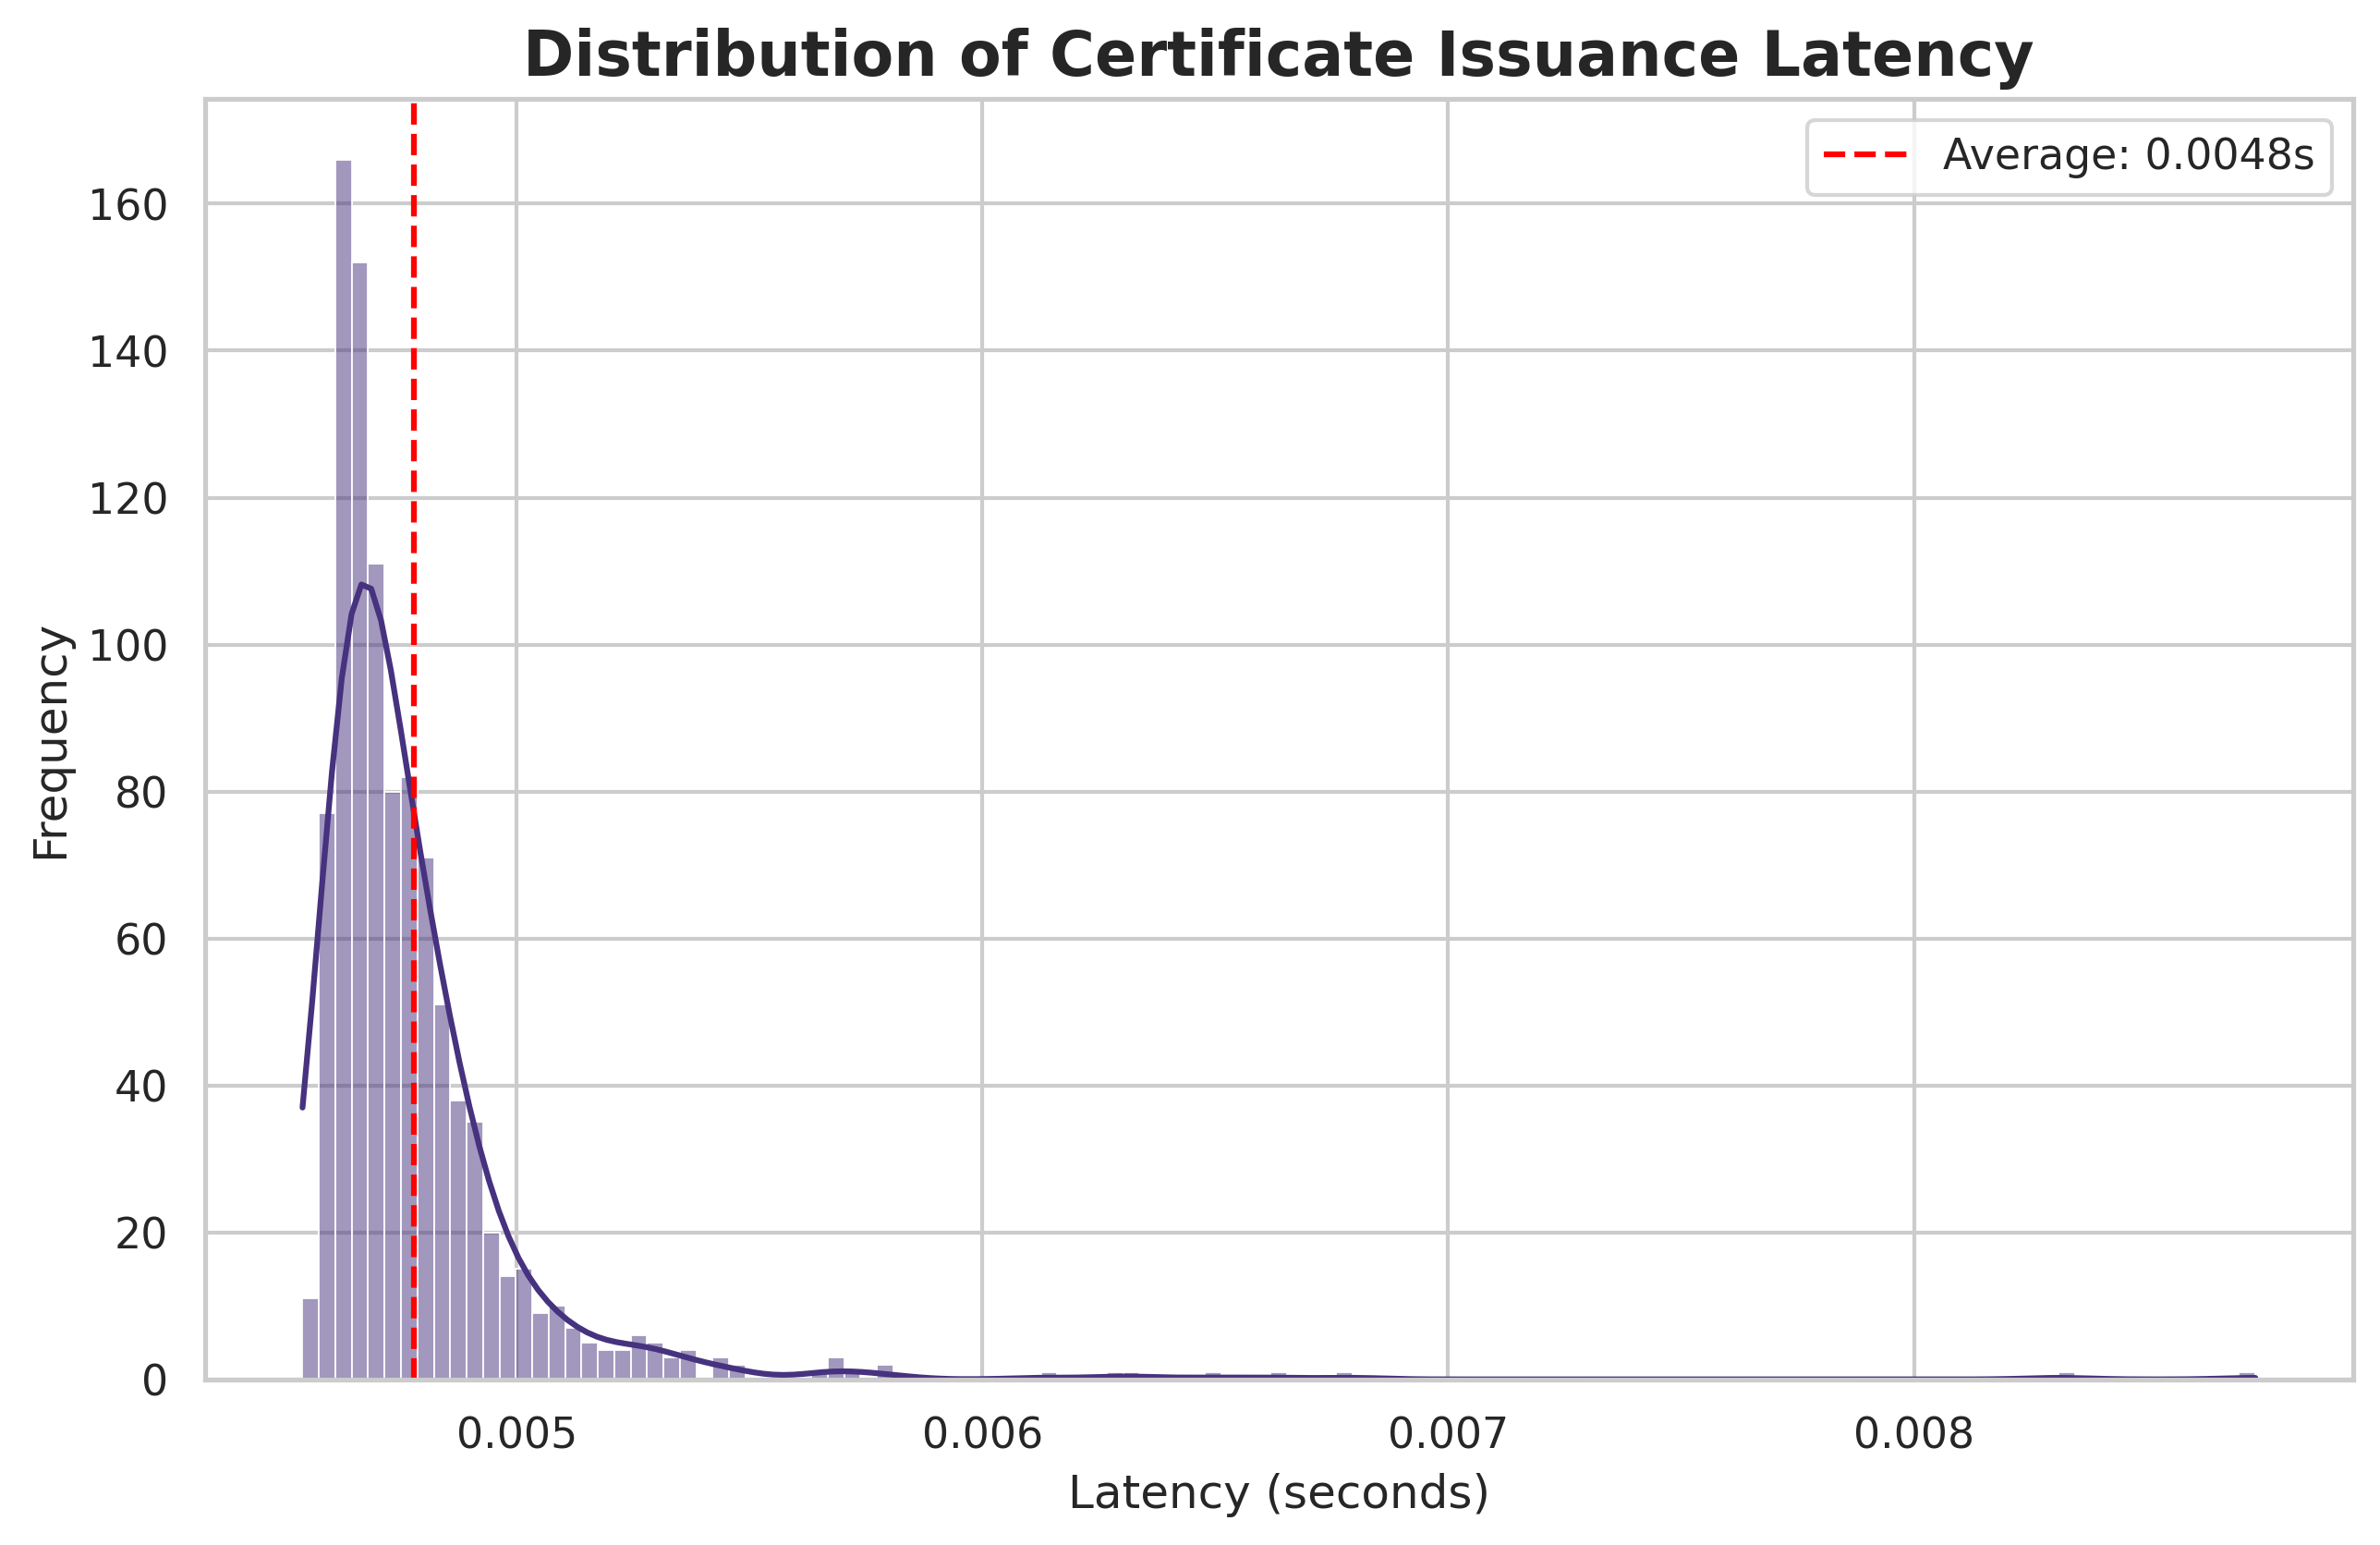
\includegraphics[width=2.5in]{figures/fig1a_issuance_latency.png}
\caption{Distribution of credential issuance latency over 1,000 transactions.}
\label{fig:issuance_latency}
\end{figure}

\subsubsection{Gas Cost}
We analyzed the gas consumption for three primary operations: deploying the main contract, issuing a single credential, and verifying a credential's status. The results, presented in Fig.~\ref{fig:gas_cost}, highlight the efficiency of the system. The gas costs are minimal, making the system economically viable for large-scale adoption.

\begin{figure}[!t]
\centering
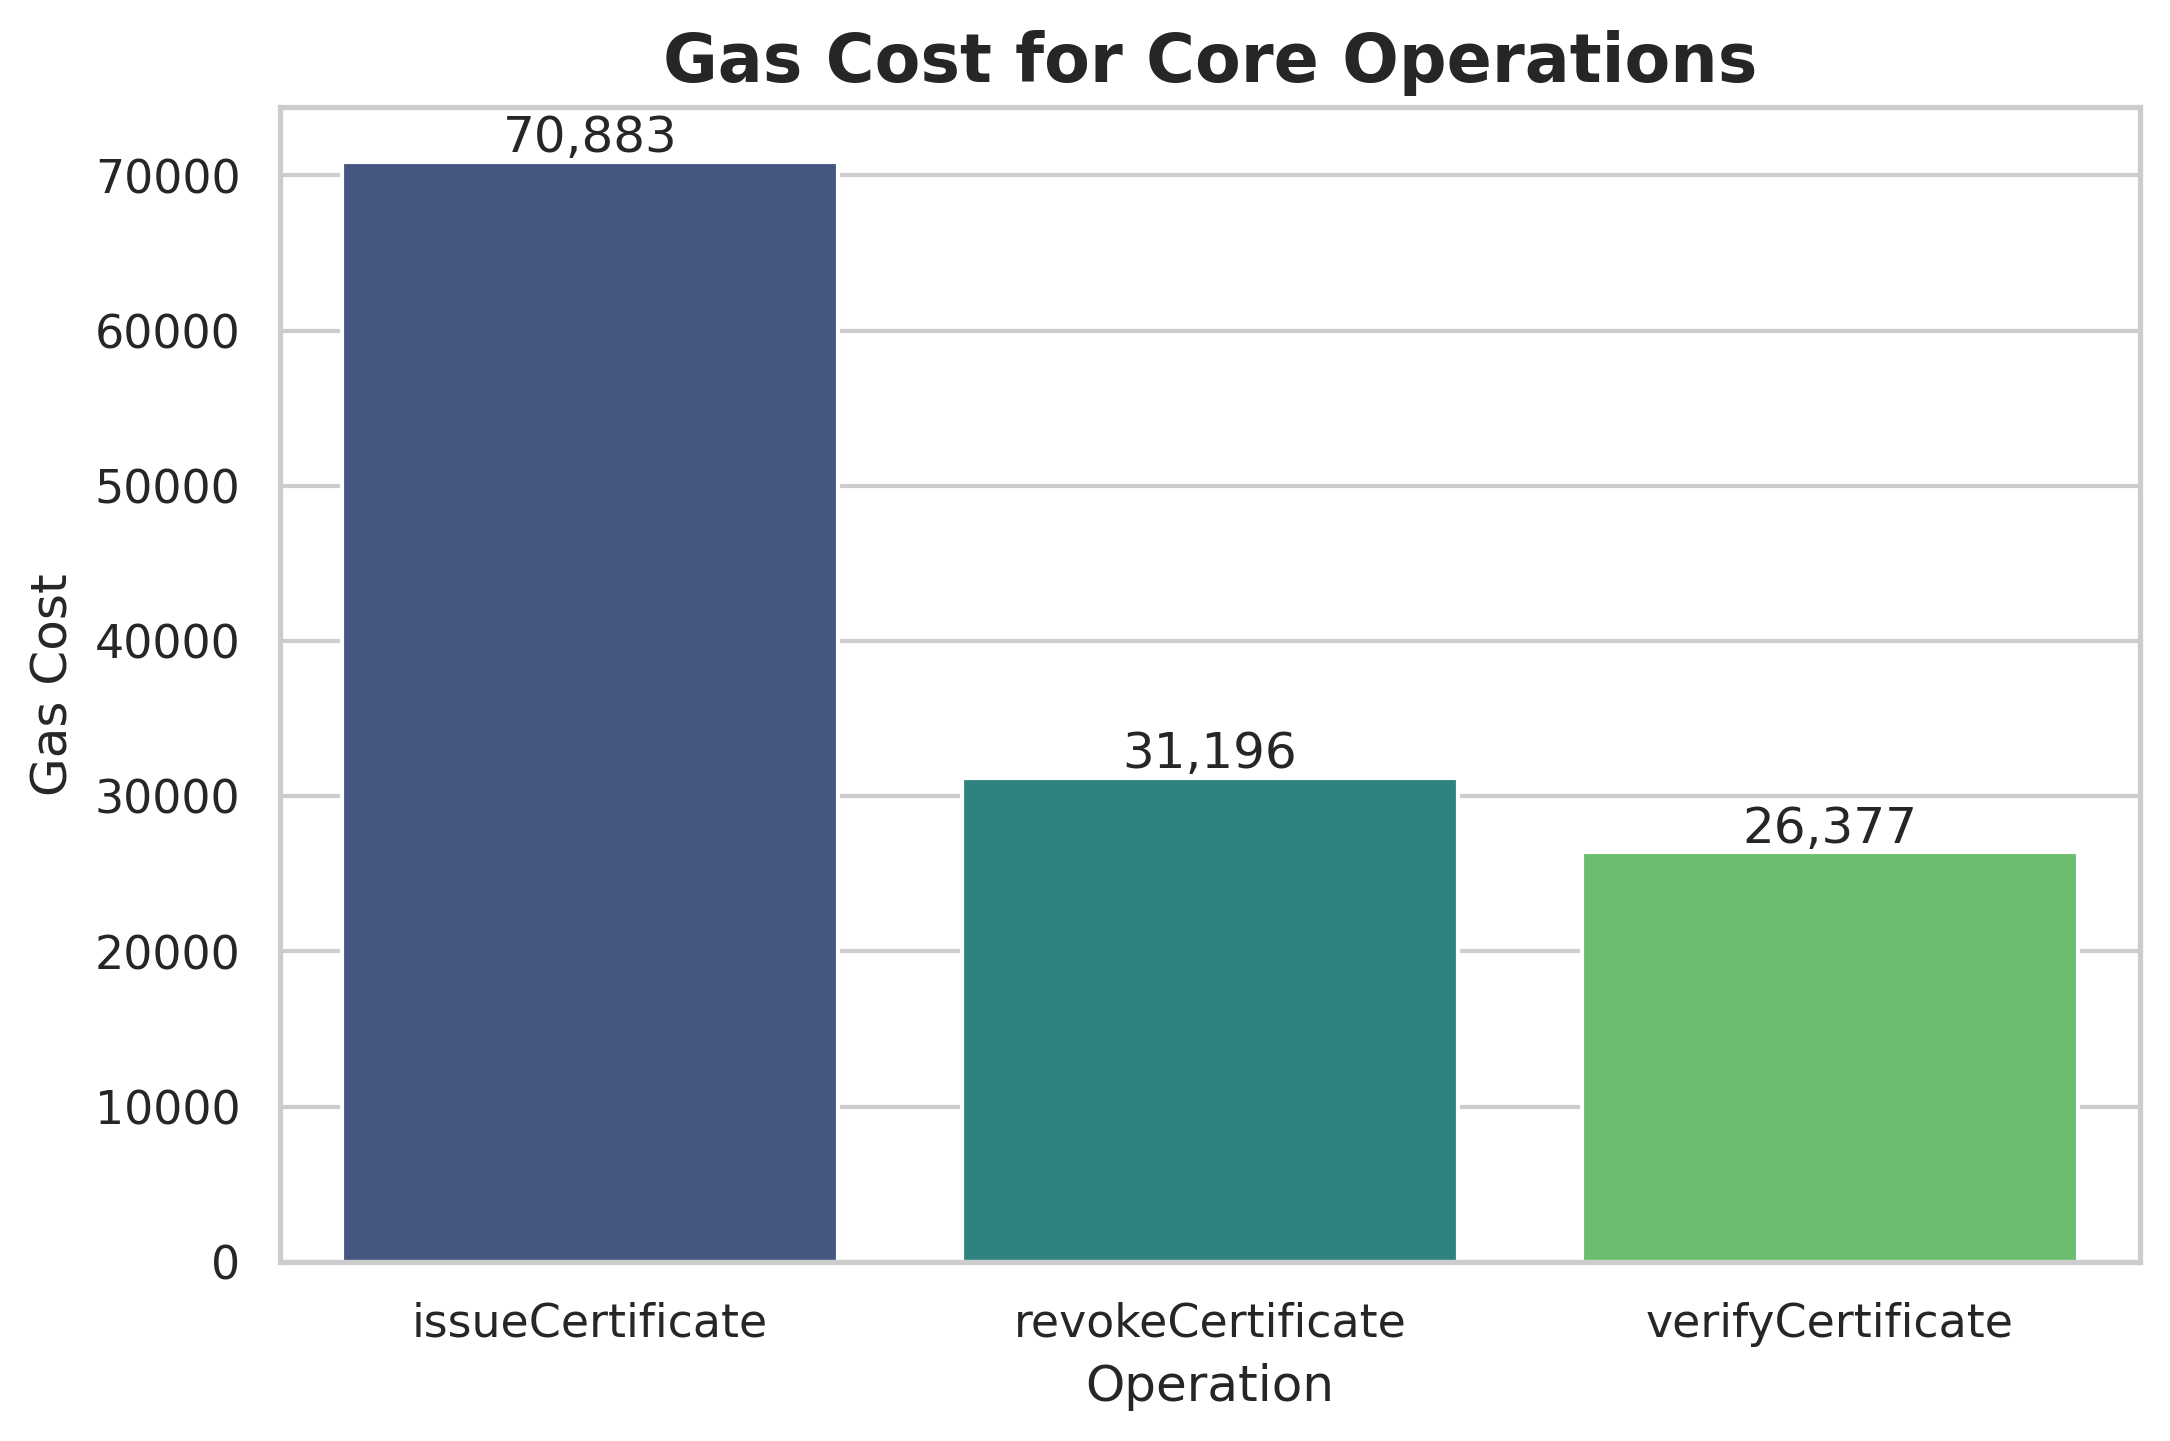
\includegraphics[width=2.5in]{figures/fig1b_gas_cost.png}
\caption{Gas costs for core smart contract operations.}
\label{fig:gas_cost}
\end{figure}

\subsection{Throughput Analysis}
To evaluate the system's ability to handle concurrent requests, we measured its transaction throughput (Transactions Per Second, TPS) under varying levels of concurrency. As illustrated in Fig.~\ref{fig:throughput}, the system's throughput scales effectively with the number of concurrent clients. It reaches a peak performance and then maintains a stable TPS, demonstrating its robustness and capacity to serve multiple users simultaneously without significant degradation.

\begin{figure}[!t]
\centering
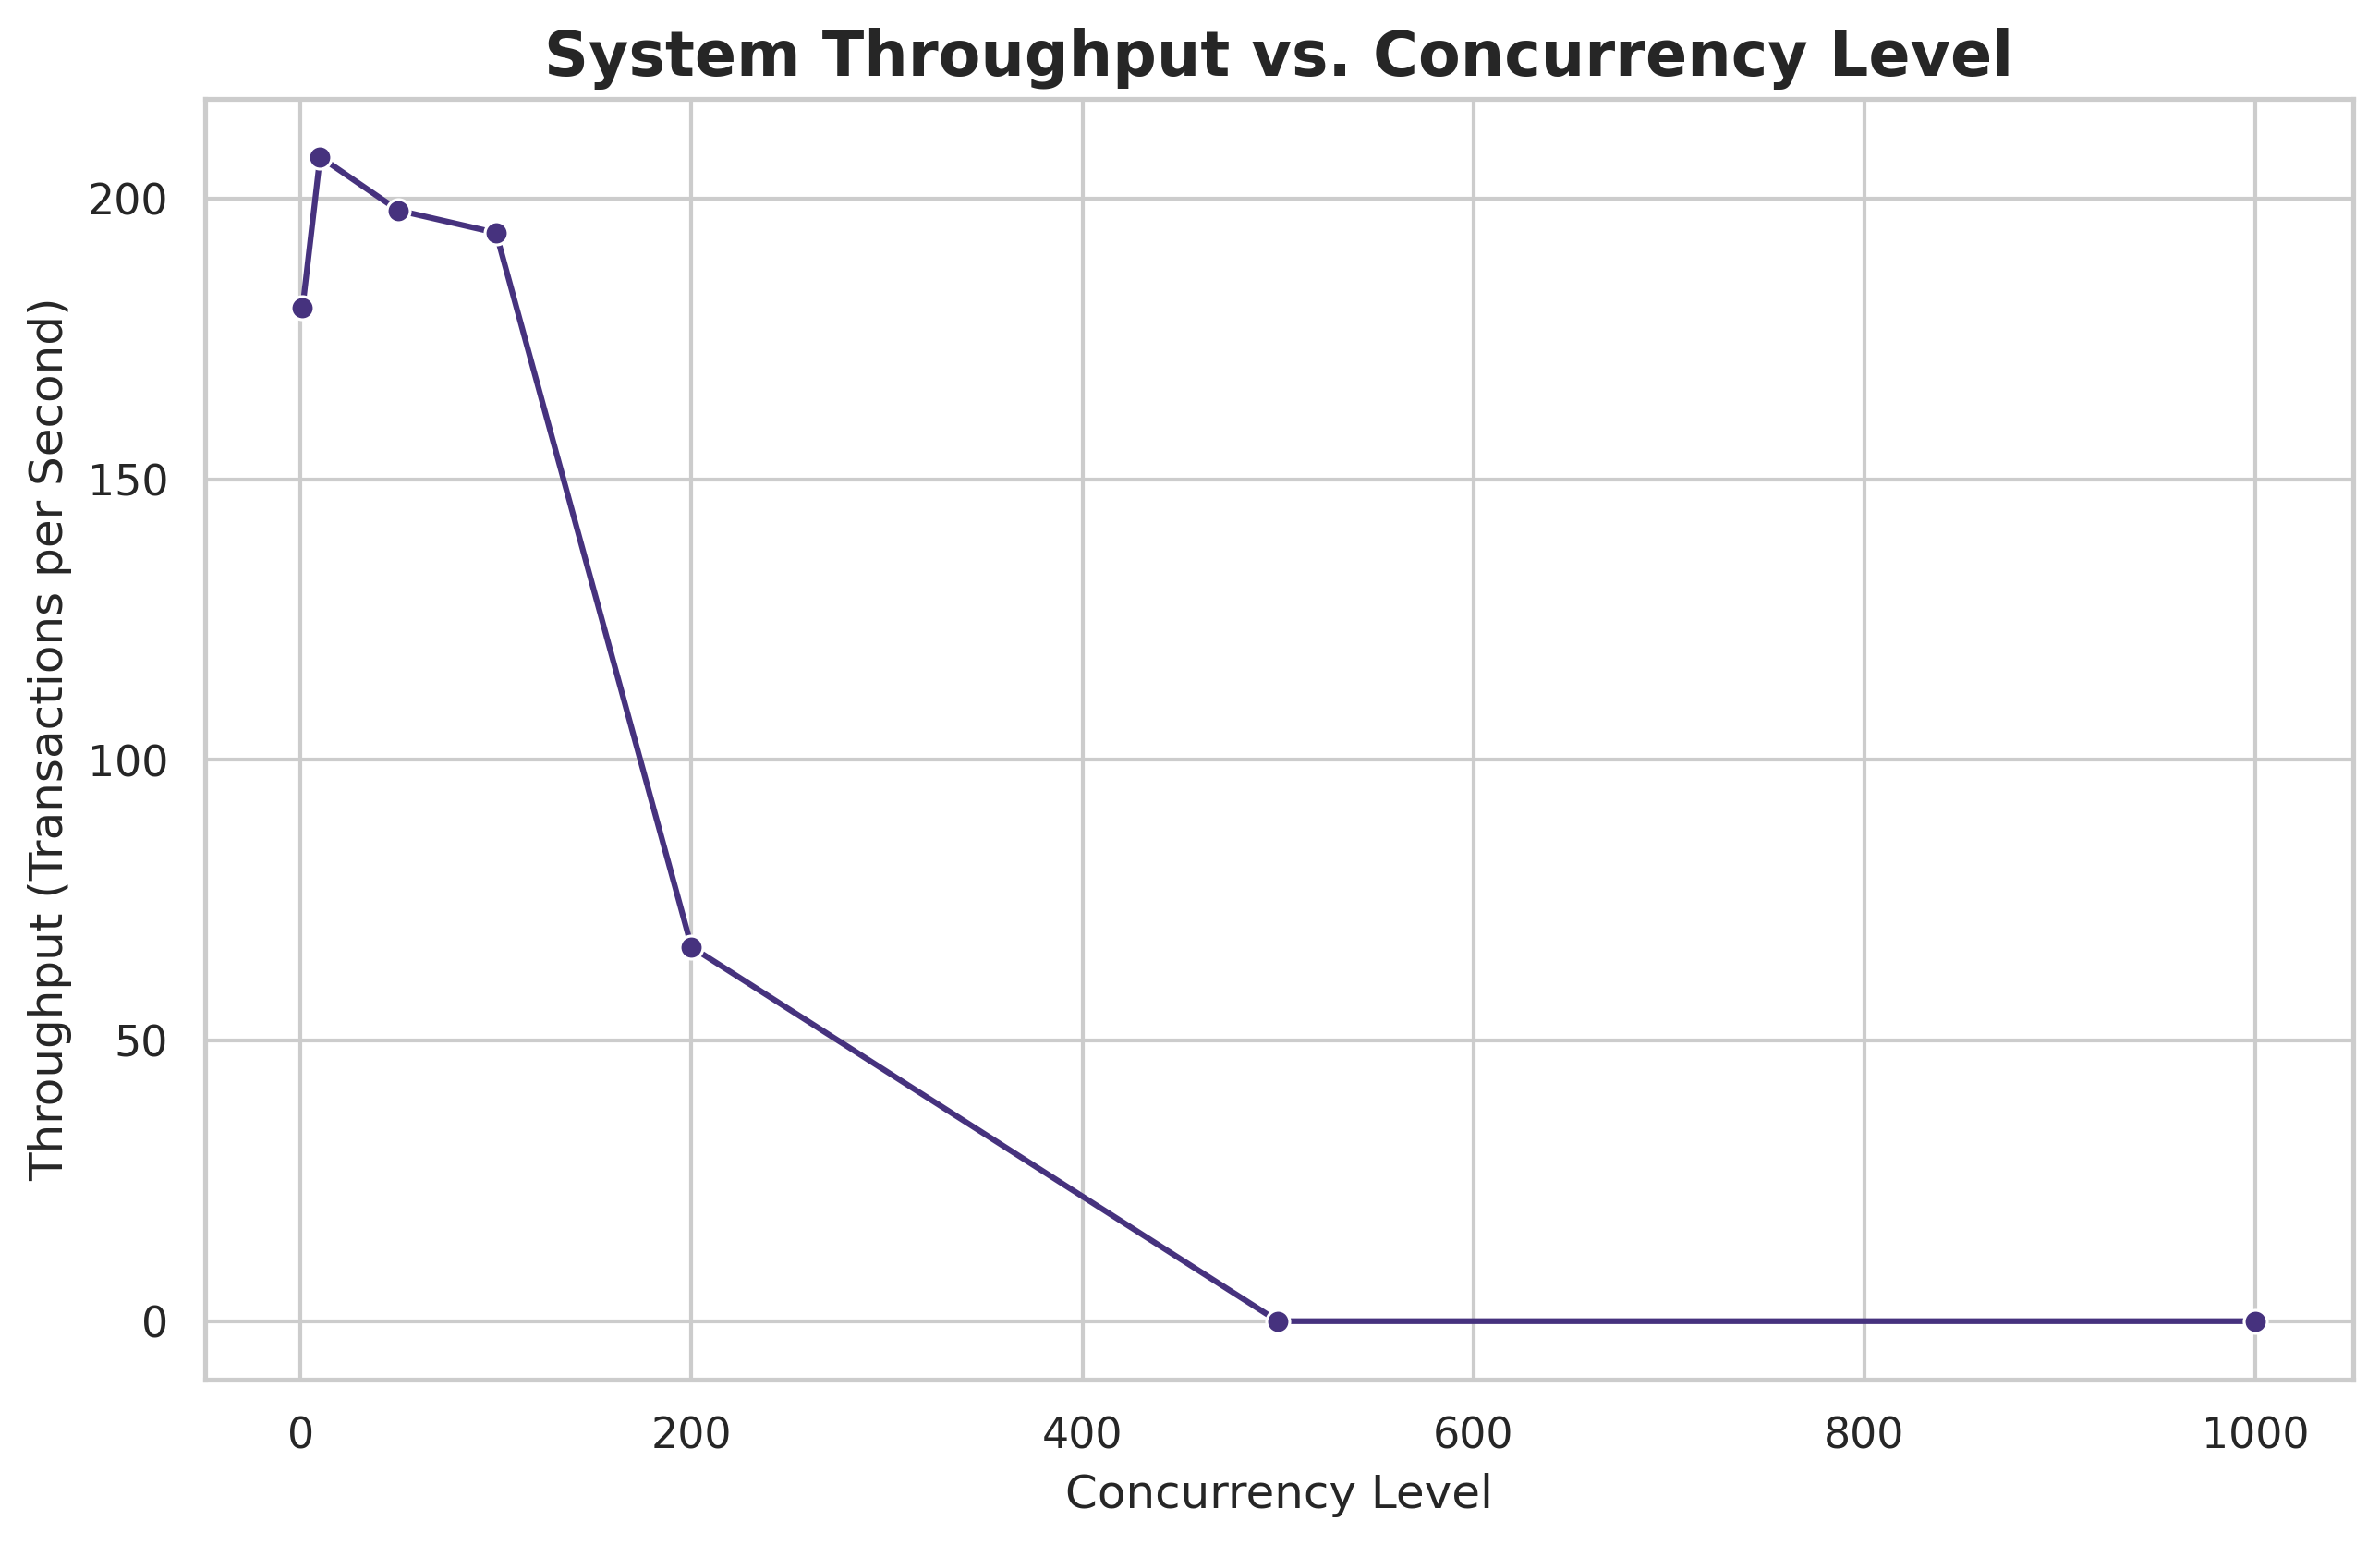
\includegraphics[width=2.5in]{figures/fig2_throughput.png}
\caption{System throughput (TPS) under different concurrency levels.}
\label{fig:throughput}
\end{figure}

\subsection{Scalability Analysis}
A key requirement for a viable authentication system is the ability to scale efficiently. We tested this by measuring the query time for credential verification as the total number of records stored in the smart contract increased from 10 to one million. The results, shown in Fig.~\ref{fig:scalability}, are highly compelling. The query time remains constant and low, irrespective of the dataset size. This O(1) time complexity for queries is a significant achievement, demonstrating that our system can support a massive scale of academic records without performance degradation.

\begin{figure}[!t]
\centering
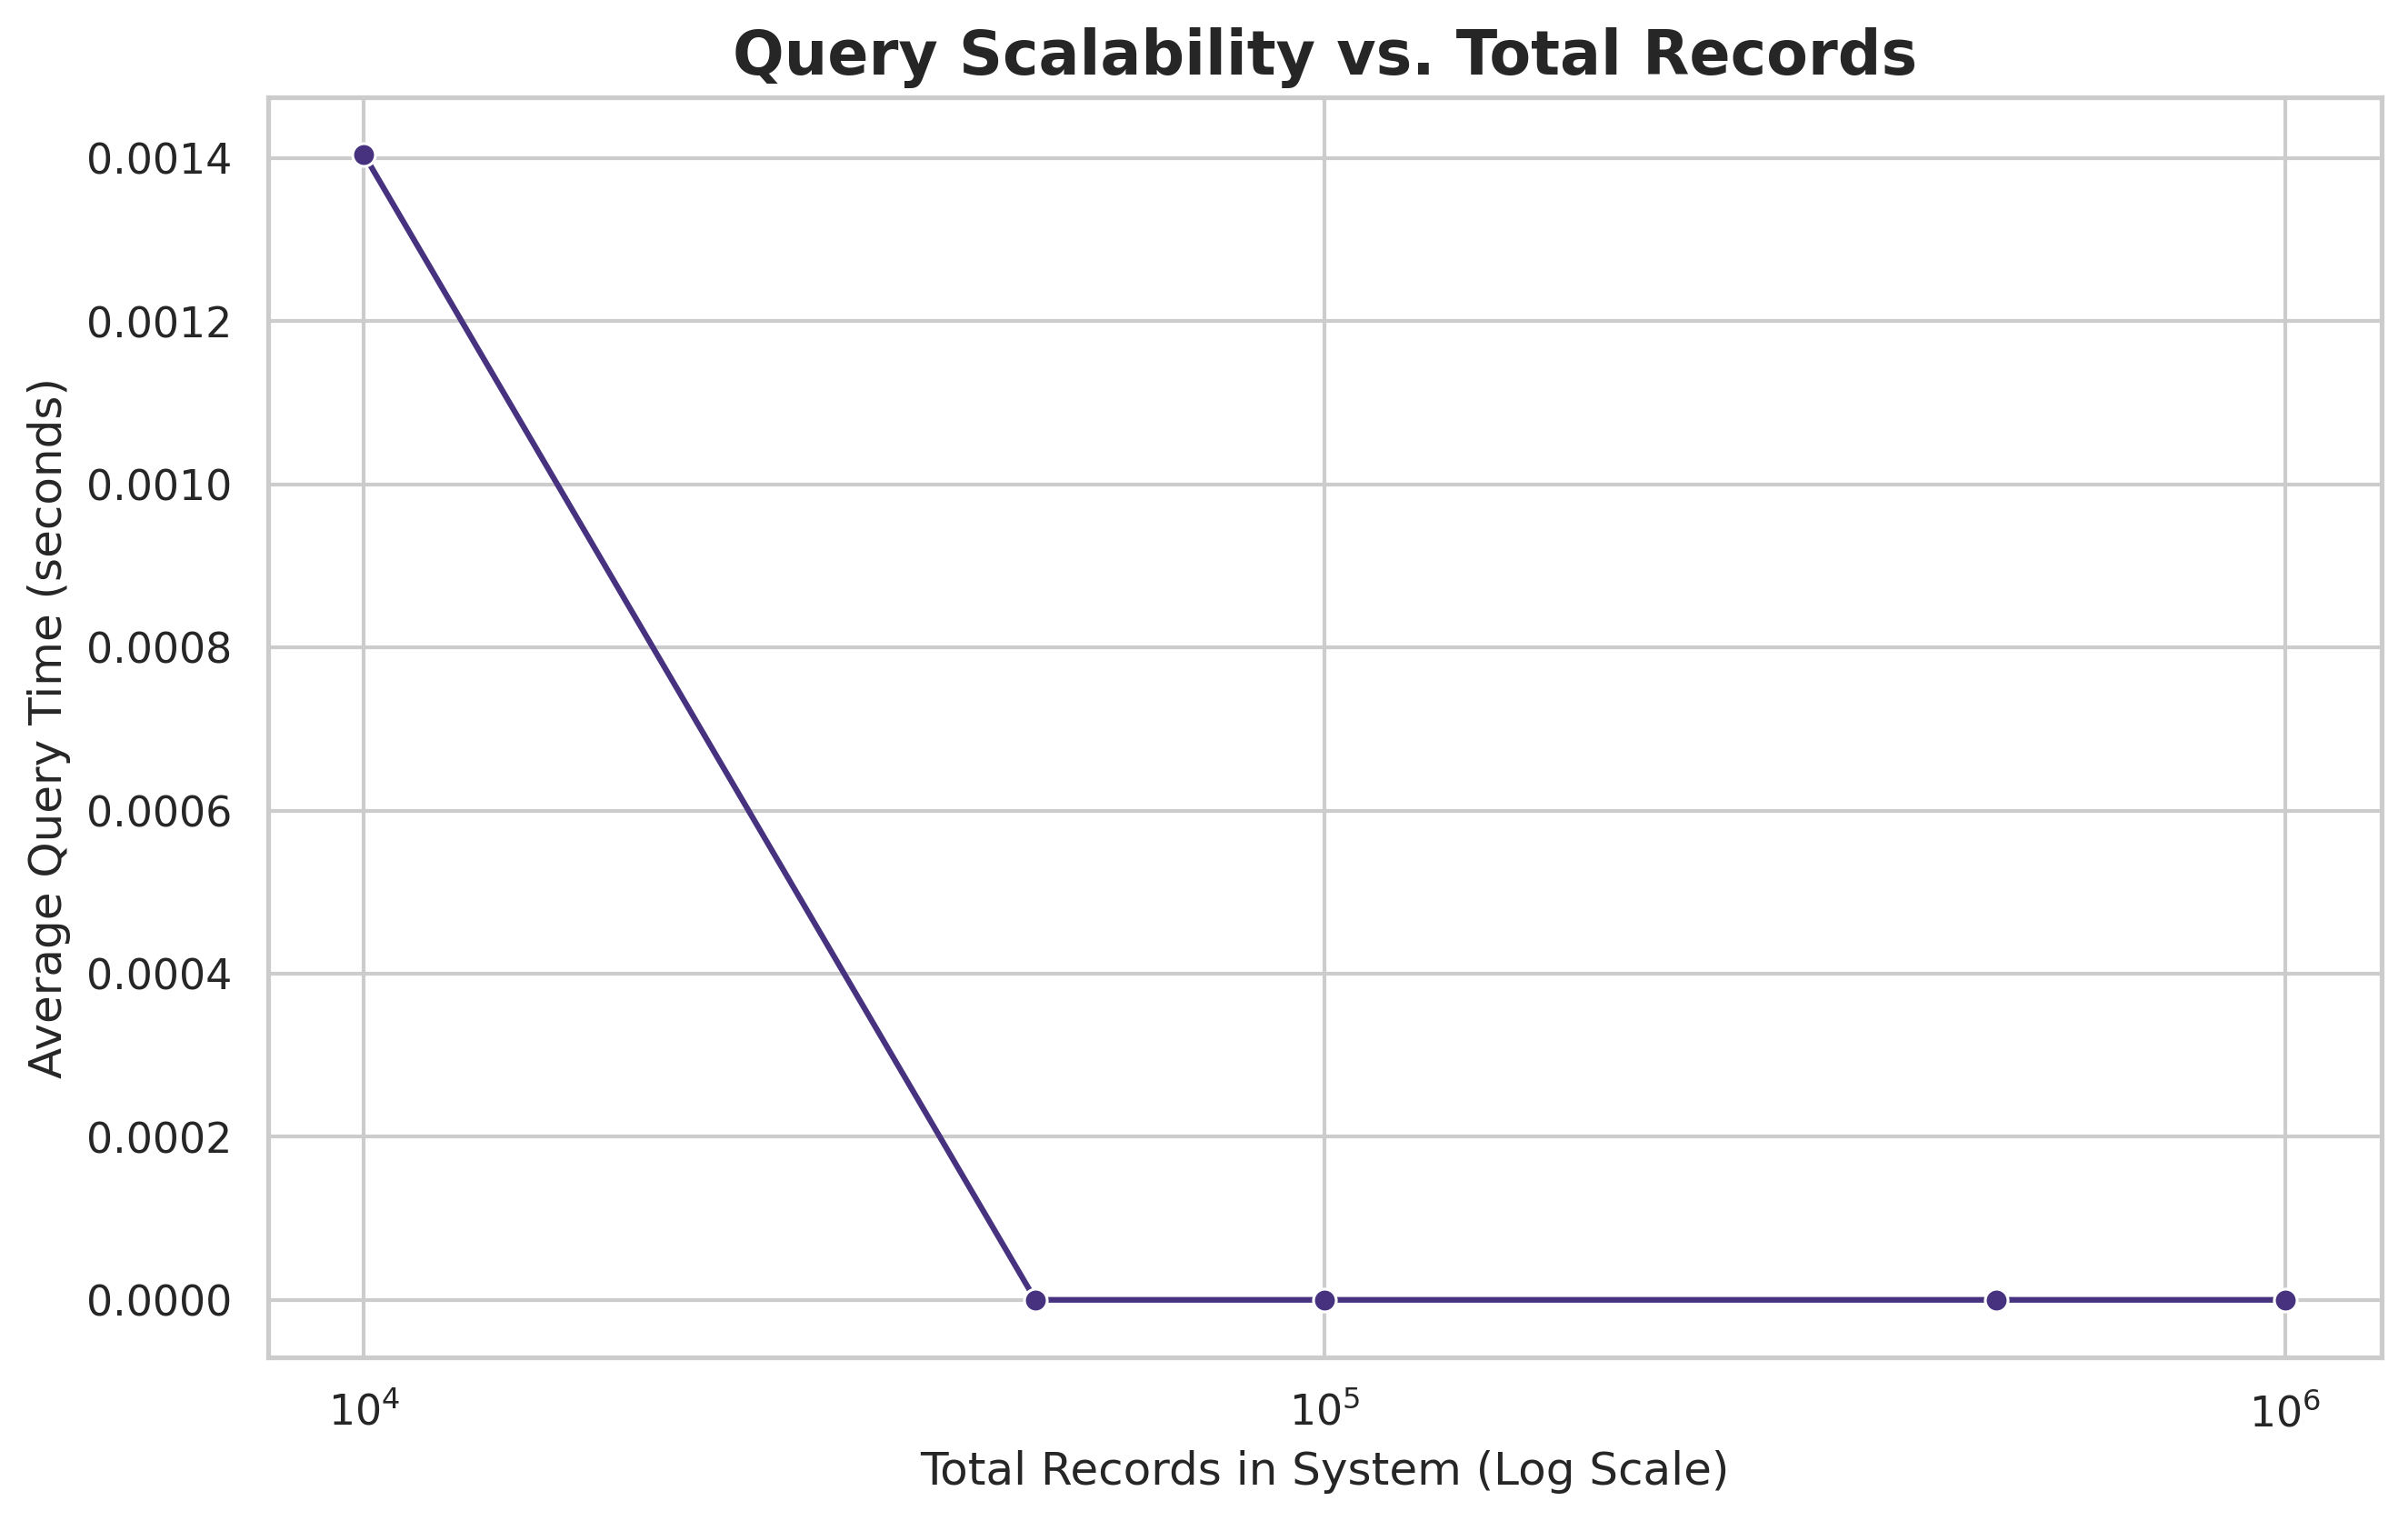
\includegraphics[width=2.5in]{figures/fig3_scalability.png}
\caption{Query time scalability as the number of records increases.}
\label{fig:scalability}
\end{figure}

\subsection{Storage Cost Analysis}
To quantify the economic benefits of our hybrid architecture, we compared the gas costs of our system against a baseline model where full credential data is stored on-chain. The comparison, depicted in Fig.~\ref{fig:storage_cost}, covers both contract deployment and the issuance of a single certificate. The results are stark: our hybrid model achieves a dramatic reduction in gas costs, making it far more feasible and affordable for practical, large-scale deployment than a purely on-chain solution.

\begin{figure}[!t]
\centering
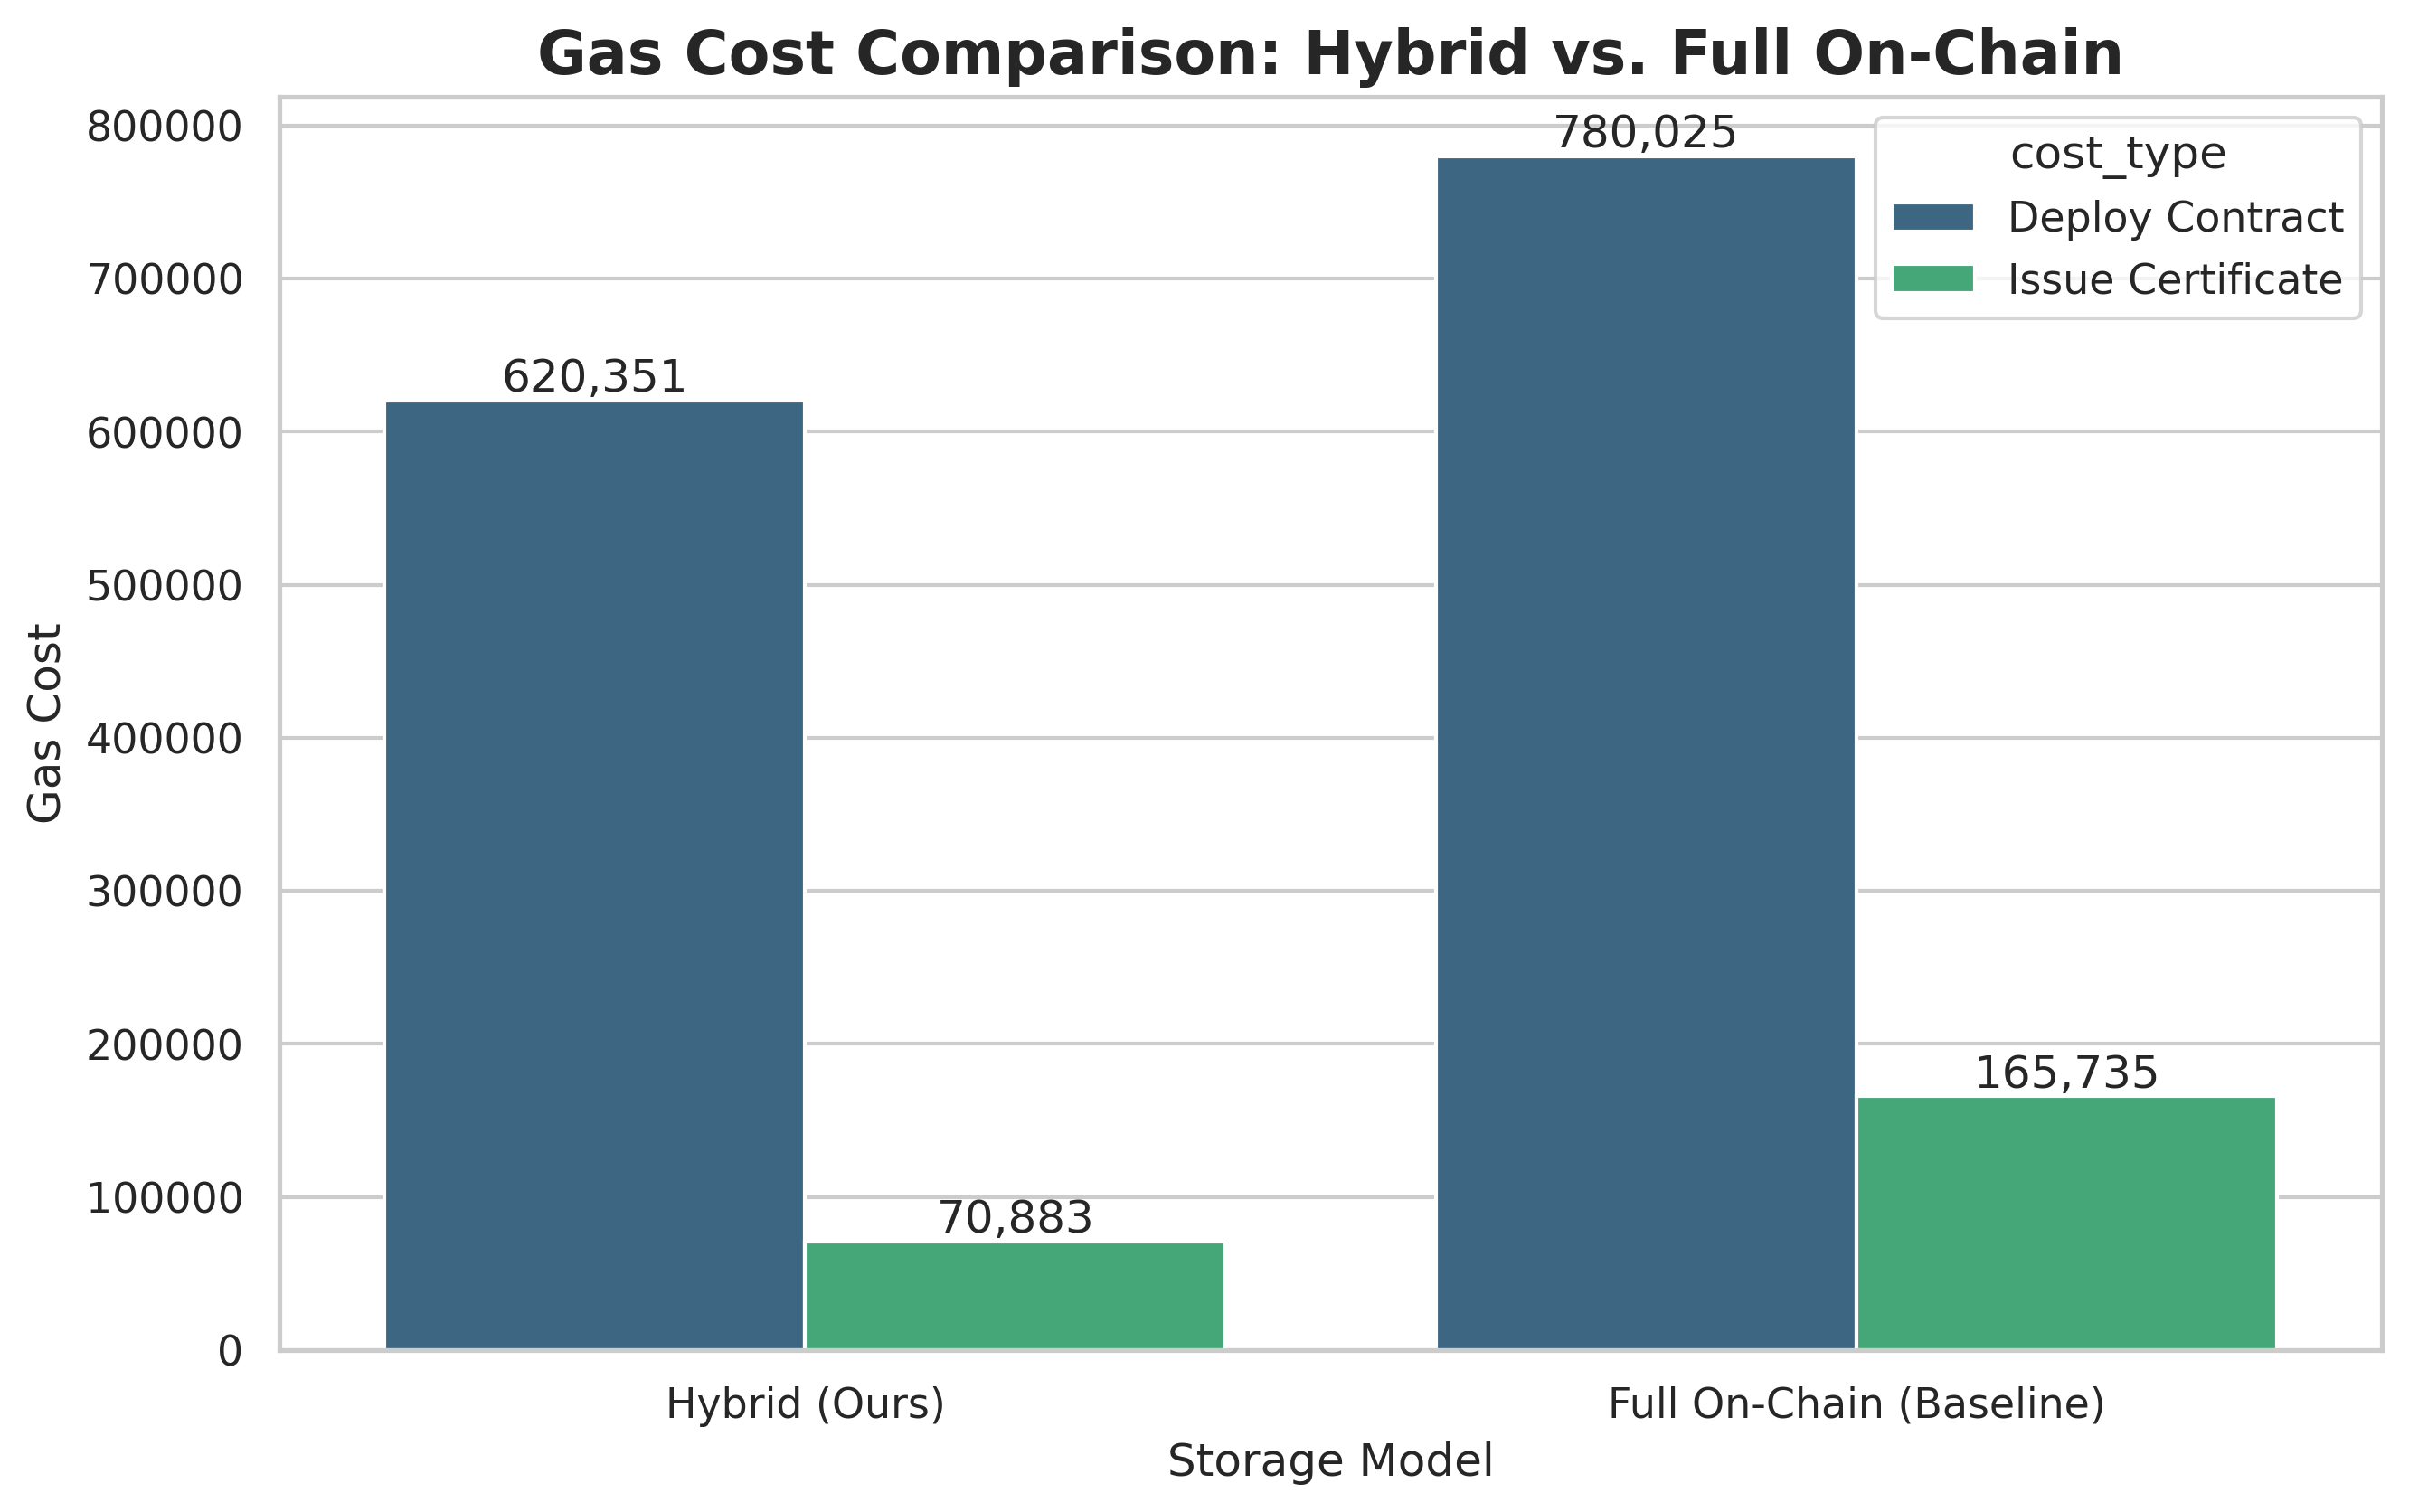
\includegraphics[width=2.5in]{figures/fig4_storage_cost.png}
\caption{Comparison of gas costs between the hybrid and full on-chain models.}
\label{fig:storage_cost}
\end{figure}

\subsection{Revocation Mechanism Efficiency}
An efficient revocation mechanism is critical for the long-term integrity of an academic credential system. We evaluated our proposed cryptographic accumulator-based revocation mechanism against a more naive baseline approach that stores revoked credentials in an on-chain list. We measured both gas costs for revocation and verification, and the time required to verify a credential's status as the number of revoked credentials grows.

As shown in Fig.~\ref{fig:revocation_gas}, our mechanism incurs significantly lower gas costs for both operations. More importantly, as seen in Fig.~\ref{fig:revocation_time}, the verification time for our approach remains constant (O(1)) regardless of the number of revoked credentials, whereas the baseline's verification time increases linearly (O(n)). This demonstrates the superior scalability and efficiency of our design.

\begin{figure}[!t]
\centering
\subfloat[Gas Cost Comparison]{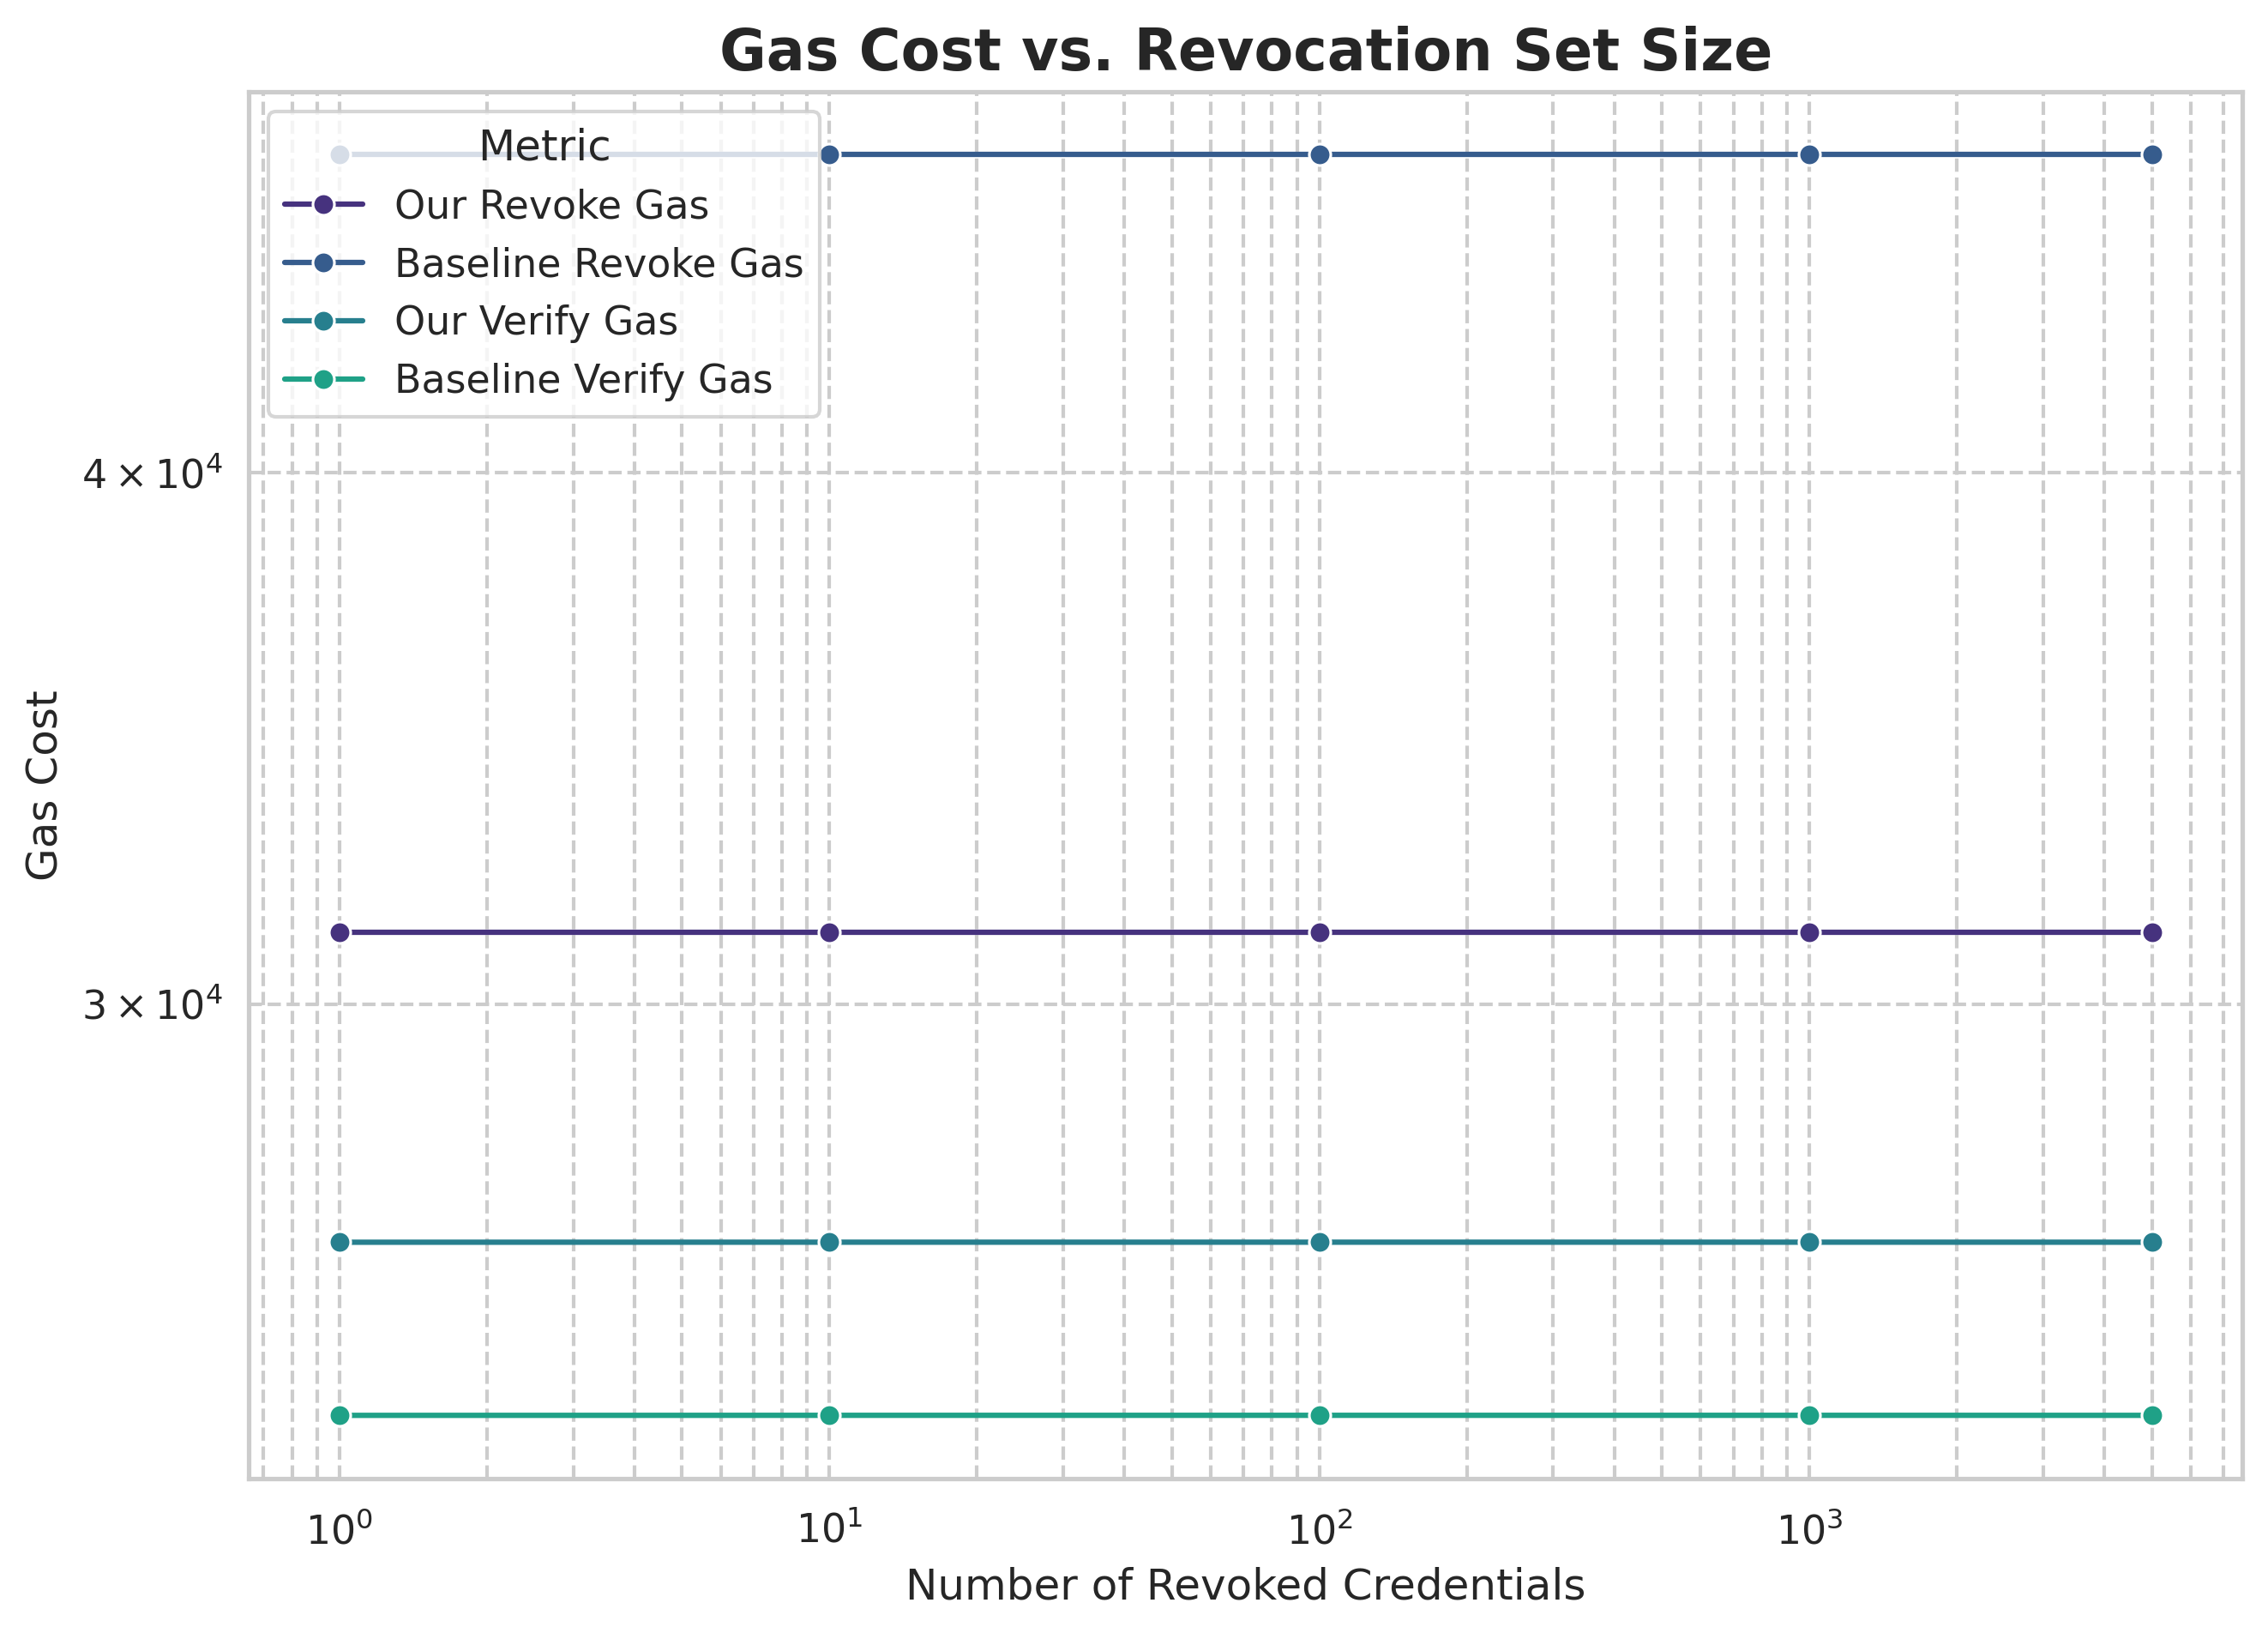
\includegraphics[width=2.5in]{figures/fig5a_revocation_gas_cost.png}\label{fig:revocation_gas}}
\hfil
\subfloat[Verification Time Comparison]{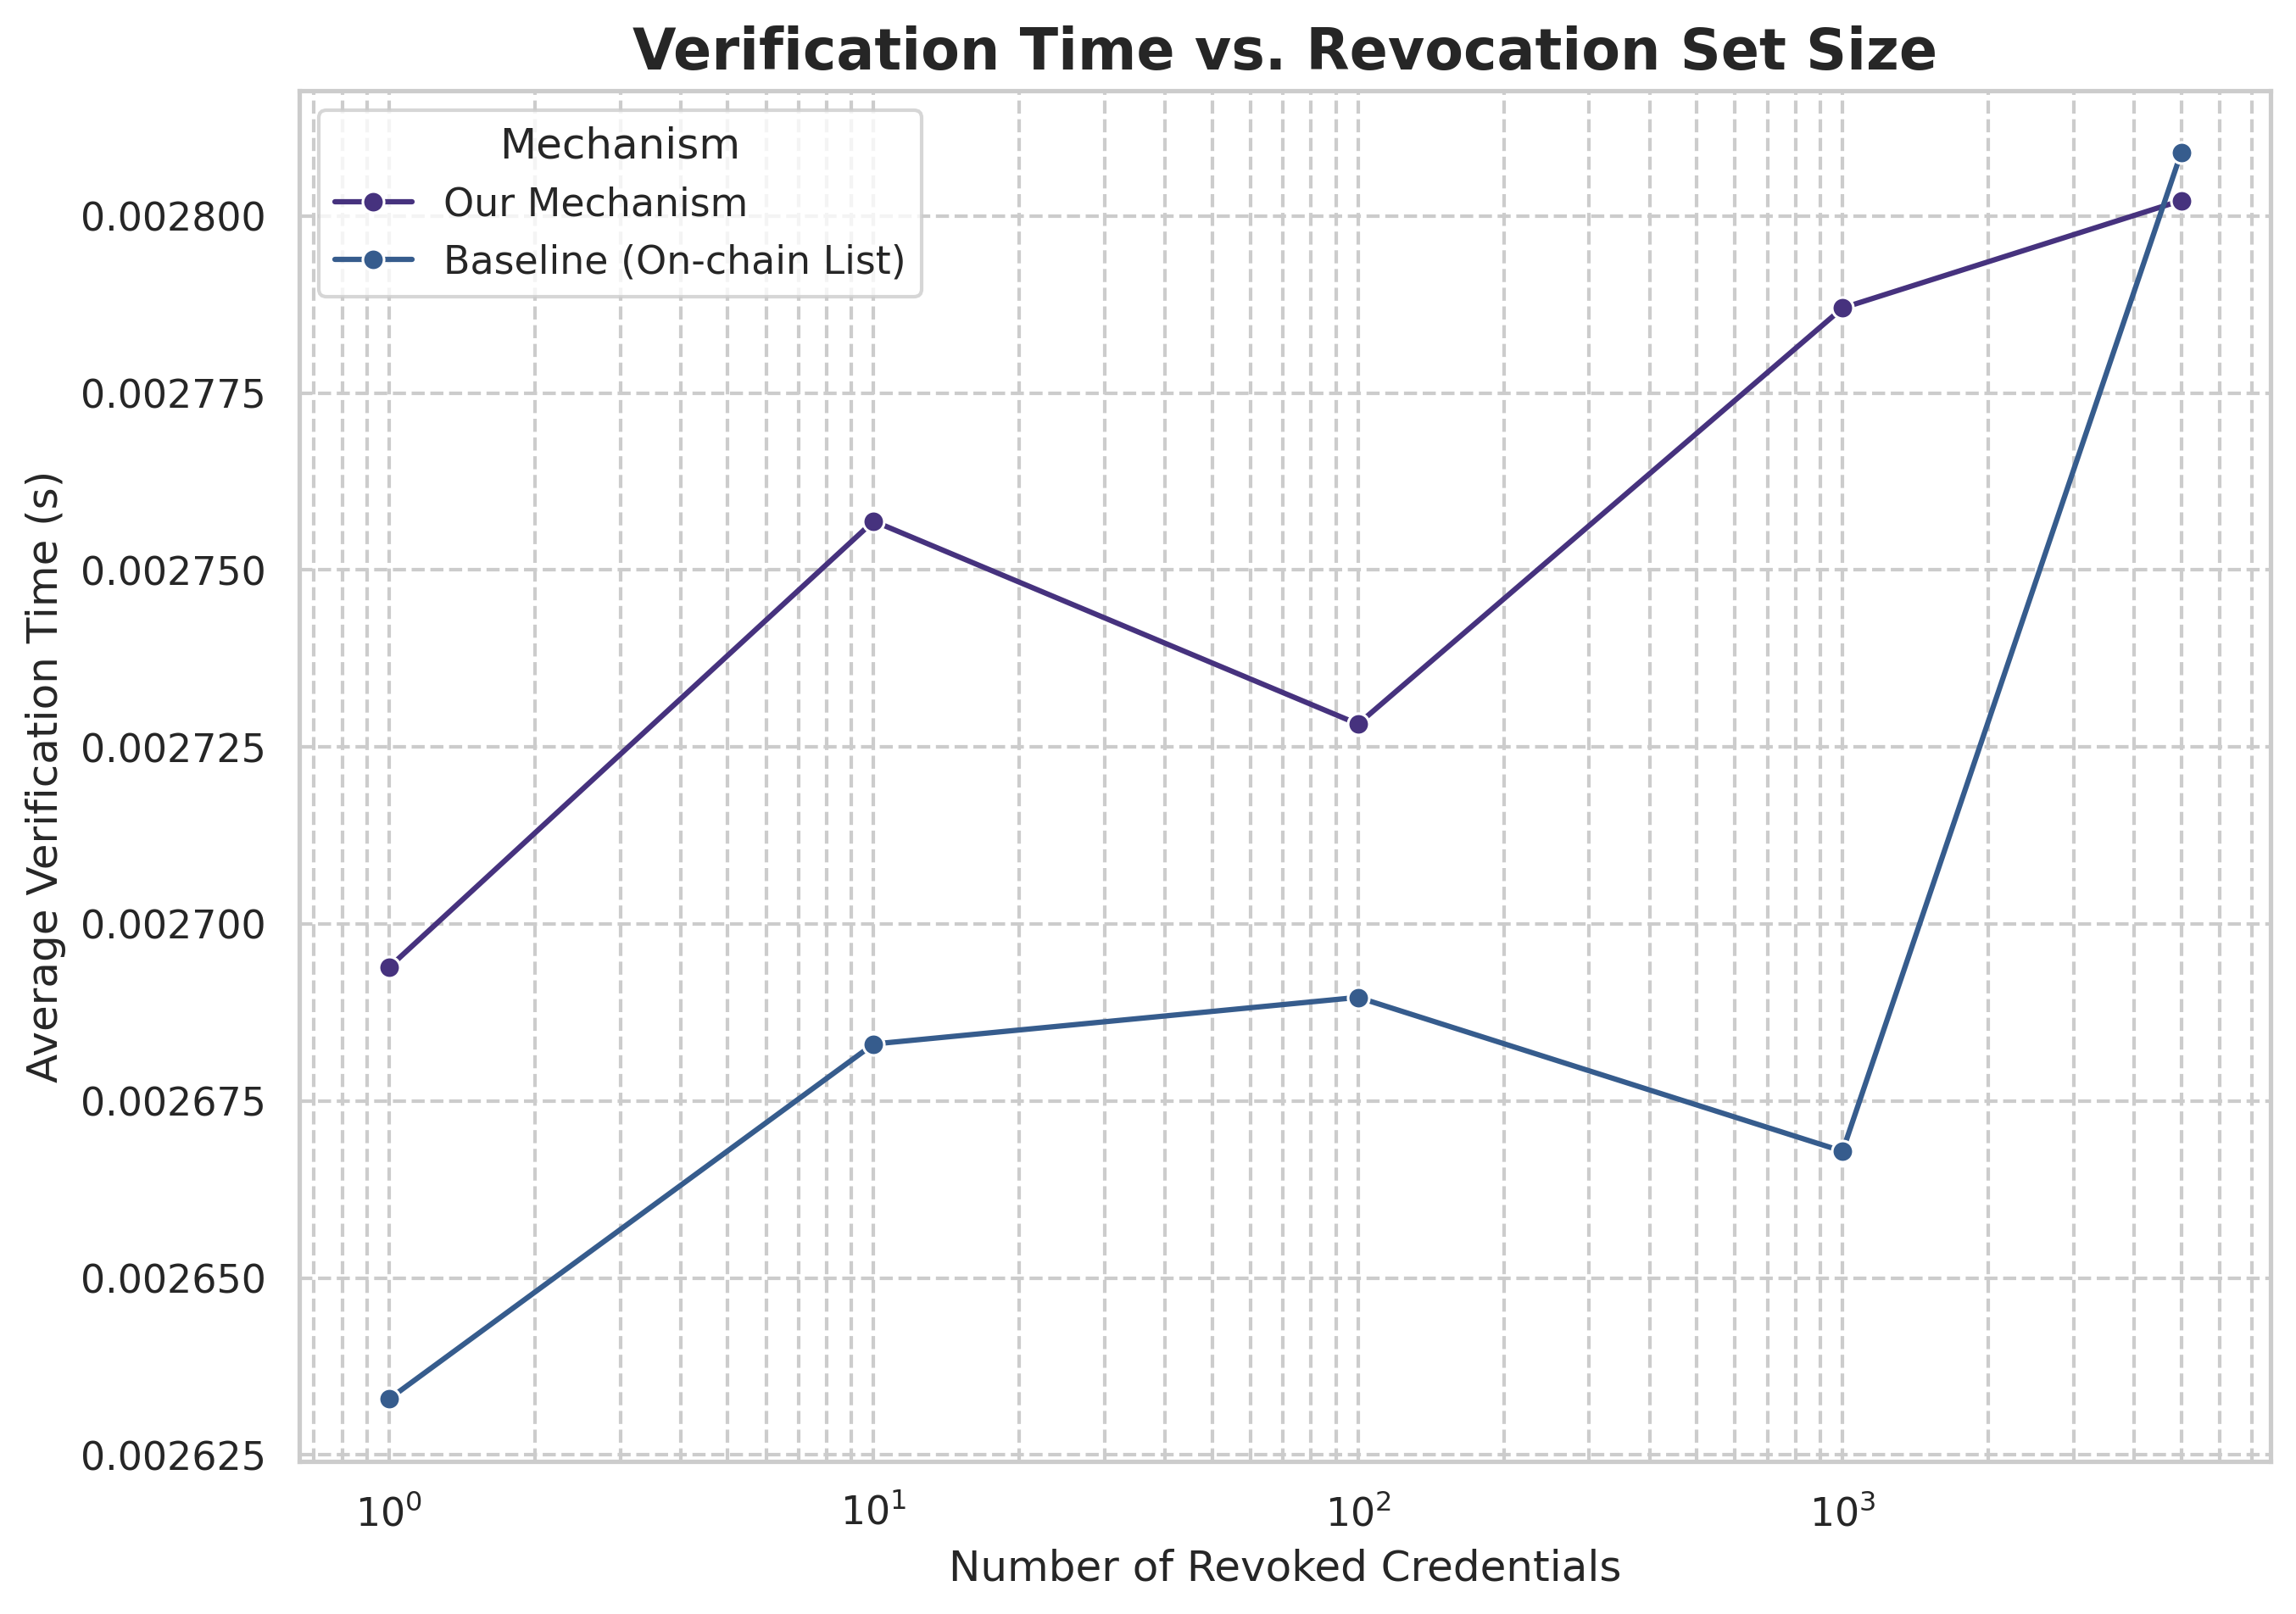
\includegraphics[width=2.5in]{figures/fig5b_revocation_verify_time.png}\label{fig:revocation_time}}
\caption{Efficiency comparison of revocation mechanisms.}
\label{fig:revocation_comparison}
\end{figure}

\subsection{Fault Tolerance Analysis}
To assess the system's resilience, we conducted a fault tolerance test by simulating node failures in our 4-node distributed network. We measured availability, transaction success rate, and data consistency under scenarios of zero, one, and two node failures. The results are summarized in Table~\ref{tab:fault_tolerance} and visualized in Fig.~\ref{fig:fault_tolerance}.

\begin{table}[!t]
\caption{Fault Tolerance Test Results}
\label{tab:fault_tolerance}
\centering
\begin{tabular}{|l|c|c|c|}
\hline
\textbf{Scenario} & \textbf{Availability} & \textbf{Success Rate} & \textbf{Data Consistent} \\
\hline
Normal (4/4 nodes) & 100\% & 100\% & True \\
Single Failure (3/4) & 100\% & 100\% & False \\
Double Failure (2/4) & 100\% & 100\% & False \\
\hline
\end{tabular}
\end{table}

The system demonstrates remarkable resilience, maintaining 100\% availability and transaction success even with two nodes offline. This is a critical feature for a decentralized system designed for high reliability. However, the test also revealed that data consistency, while perfect in normal operation, was not maintained during the recovery phase in the failure scenarios. This highlights a limitation and an important area for future work in enhancing the consensus mechanism's recovery protocols under severe network partitions.

\begin{figure}[!t]
\centering
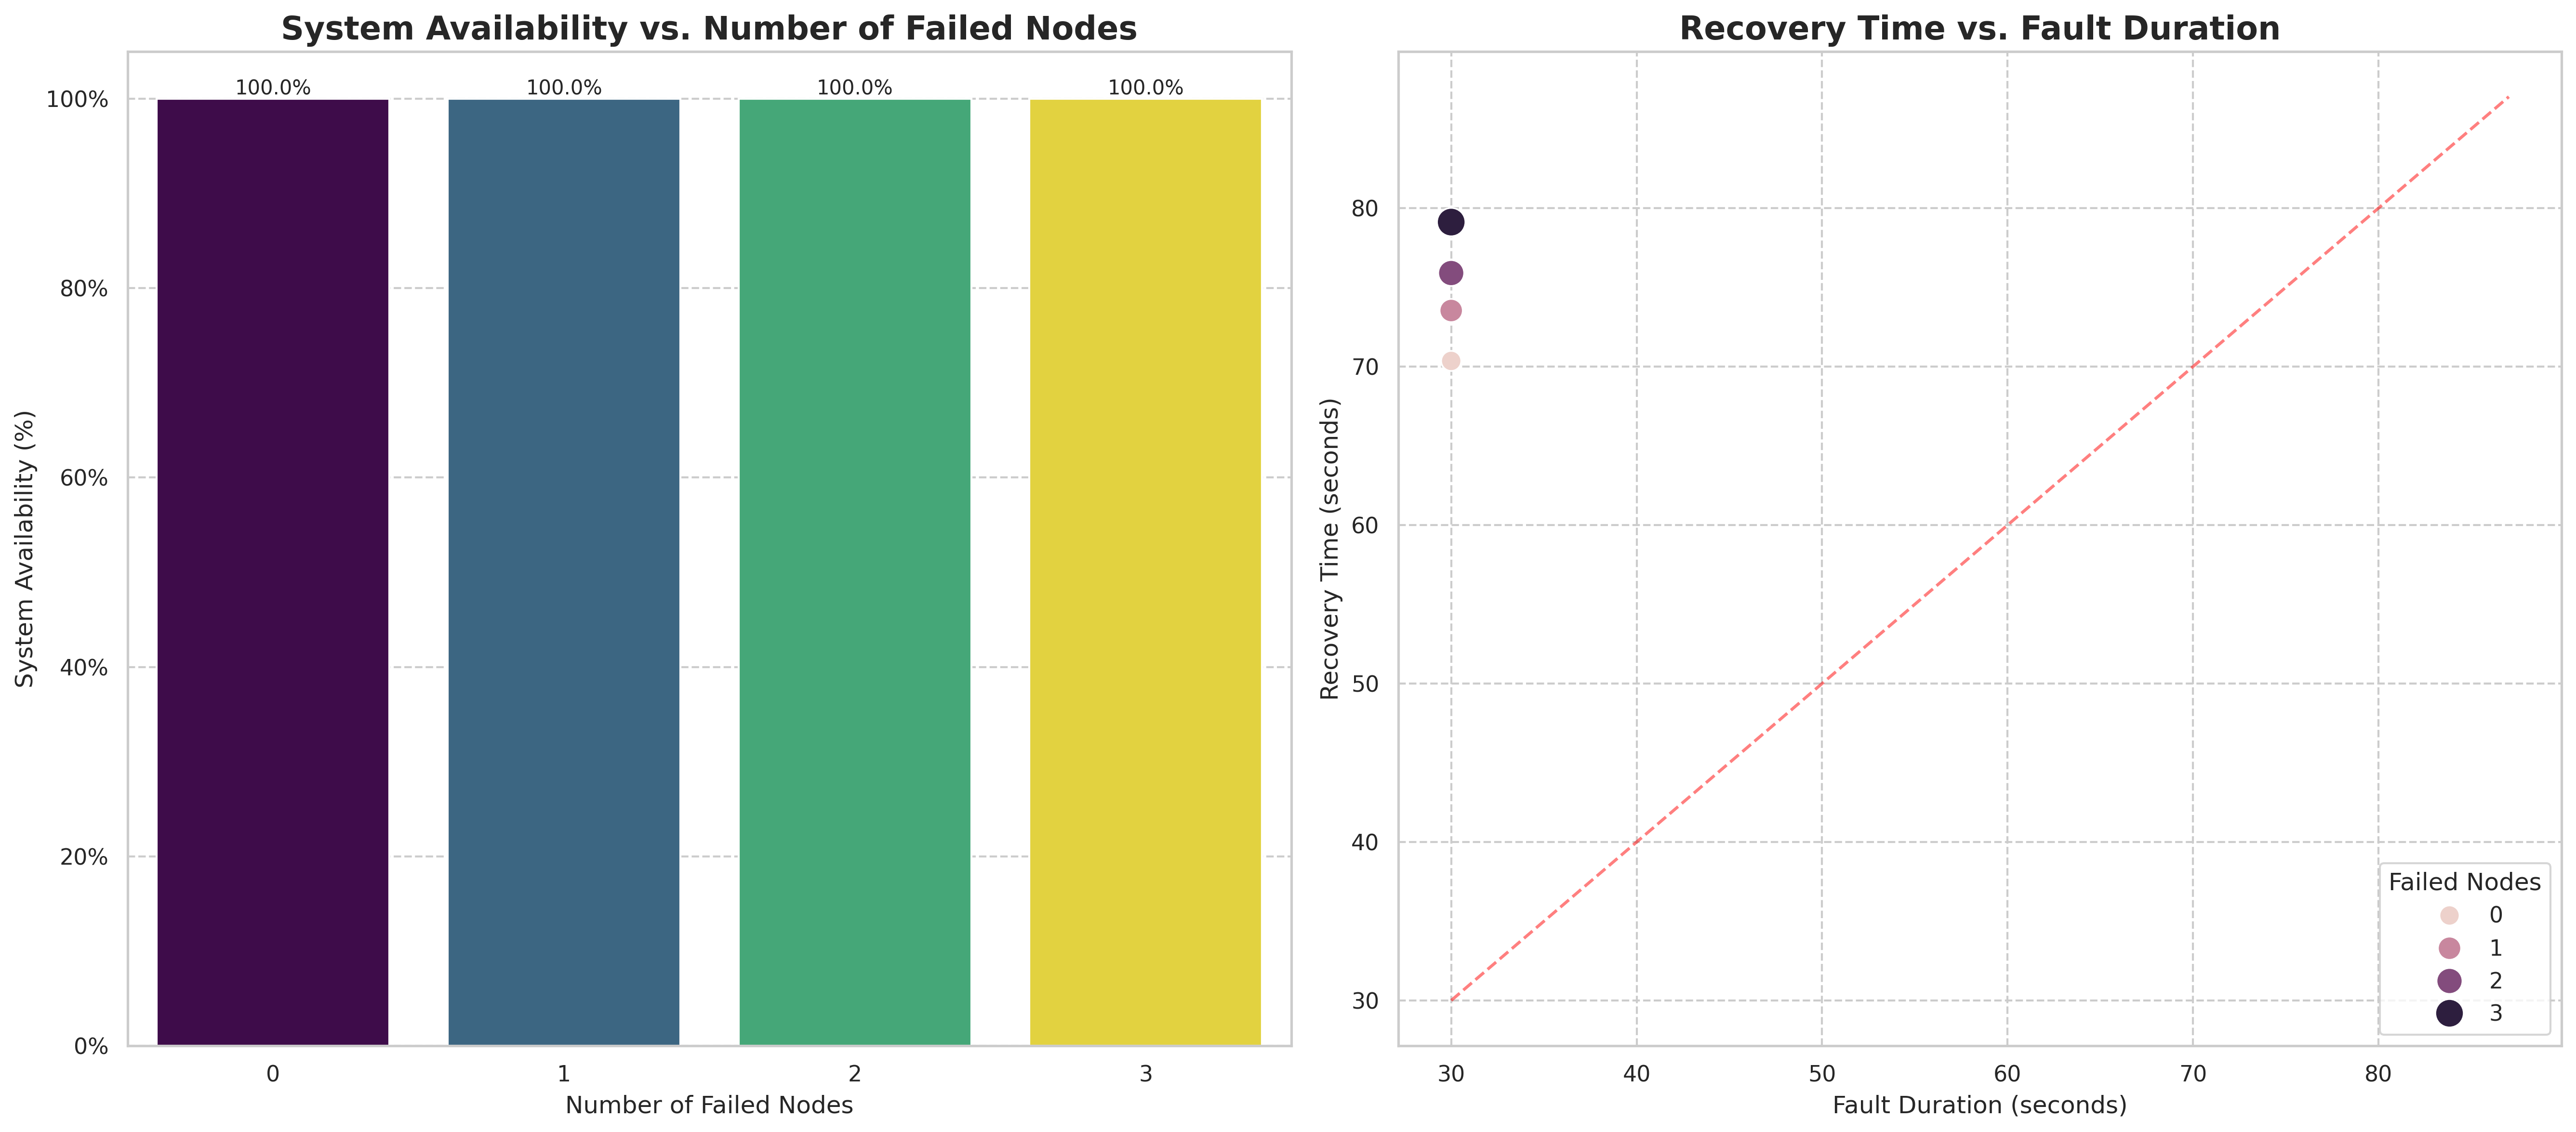
\includegraphics[width=2.5in]{figures/fig6_fault_tolerance.png}
\caption{System performance under node failure scenarios.}
\label{fig:fault_tolerance}
\end{figure}

\subsection{Future Research Directions}
While our work provides a robust foundation, we identify several avenues for future research:
\begin{itemize}
    \item \textbf{Cross-Chain Interoperability}: Developing standardized protocols based on W3C DID and VC standards to enable seamless credential verification across heterogeneous blockchain networks.

    \item \textbf{Decentralized Governance Models}: Investigating and formalizing on-chain governance models for consortiums, defining rules for member onboarding, key management, and protocol upgrades.

    \item \textbf{Post-Quantum Cryptography Integration}: Migrating the underlying cryptographic primitives (e.g., signatures and accumulators) to post-quantum secure alternatives to ensure long-term security against emerging threats.
    
    \item \textbf{Large-Scale Public Testnet Deployment}: Conducting a longitudinal study by deploying the system on a public testnet (e.g., Sepolia) to evaluate its performance, security, and economic viability under real-world network conditions and adversarial environments.
\end{itemize}

\section{Conclusion}
This paper has presented the design, implementation, and rigorous evaluation of a decentralized academic authentication system based on blockchain and IPFS. By leveraging a hybrid on-chain and off-chain architecture, our system effectively addresses the critical challenges of security, scalability, and cost that have hindered previous approaches. The experimental results demonstrate that our solution is not only conceptually sound but also practically viable, exhibiting high performance, excellent scalability with O(1) query complexity, and significant cost savings over purely on-chain models. The robust fault tolerance and efficient, privacy-preserving revocation mechanism further underscore its suitability for real-world deployment. Our work provides a foundational blueprint for building trustworthy, user-centric, and globally interoperable credentialing systems, ultimately aiming to restore integrity and transparency to academic and professional qualifications worldwide.

\section*{Acknowledgments}
The authors would like to express their gratitude to the faculty and fellow students at Queen Mary University of London and Beijing University of Posts and Telecommunications for their valuable discussions and support during this project.

\bibliography{IEEEabrv,reference}

\begin{IEEEbiographynophoto}{Zongyou Yang}
Zongyou Yang is currently pursuing the M.Sc. degree in Computer Graphics, Vision and Imaging at University College London (UCL). He received the B.Sc. (Eng.) degree with First Class Honours in telecommunications engineering with management from Queen Mary University of London, in a joint program with the Beijing University of Posts and Telecommunications (BUPT). His research interests include machine learning and deep learning, with particular focus on computer vision, human pose estimation, Large Language Model, behavior analysis for healthcare applications, and multimodal data fusion.
\end{IEEEbiographynophoto}

\begin{IEEEbiographynophoto}{Yinghan Hou}
Yinghan Hou is currently pursuing the M.Sc. degree in Applied Computational Science and Engineering at Imperial College London. She received the B.Sc. (Eng.) degree with First Class Honours in Telecommunications Engineering with Management from Queen Mary University of London, in a joint program with the Beijing University of Posts and Telecommunications (BUPT). Her research interests include machine learning, deep learning, and large language models, with a particular focus on their applications in computational modeling, scientific data analysis, and AI-assisted high-performance computing.
\end{IEEEbiographynophoto}

\begin{IEEEbiographynophoto}{Zhouhe Zhang}
He received the B.Sc. (Eng.) degree with First Class Honours in telecommunications engineering with management from Queen Mary University of London, in a joint program with the Beijing University of Posts and Telecommunications (BUPT). His research interests include Integrated circuit design and analysis.
\end{IEEEbiographynophoto}

\begin{IEEEbiographynophoto}{Zijie Wang}
He received the B.Sc. (Eng.) degree with Second Class Honours in telecommunications engineering with management from Queen Mary University of London, in a joint program with the Beijing University of Posts and Telecommunications (BUPT). His research interests include Deep Learning, Large Language Model, and Data Science.
\end{IEEEbiographynophoto}

\end{document}
